\documentclass[12pt]{article}
\usepackage[letterpaper]{geometry}
\usepackage{times}
\geometry{top=1.0in, bottom=1.0in, left=1.0in, right=1.0in}
\usepackage{setspace}
\doublespacing
\usepackage[utf8]{inputenc}
\usepackage{algorithm} 
\usepackage{algpseudocode} 
\usepackage{hyperref}
\usepackage{tabularx}
\usepackage{listings}
\usepackage{hyperref}
\newcommand{\comment}[1]{}

\usepackage{lmodern} % for bold teletype font
\usepackage{minted}

%include packages for graphics
\usepackage{blindtext}
\usepackage[english]{babel}
\usepackage{graphicx}
\usepackage{comment}
\usepackage{array}
\graphicspath{ {figures/} }

\addto\captionsenglish{
\renewcommand{\listfigurename}{List of plots}
}

%Fancy-header package to modify header/page numbering
\usepackage{fancyhdr}
\pagestyle{fancy}
\lhead{} 
\chead{} 
\rhead{Chen, Chen, Yan, Yang \thepage} 
\lfoot{} 
\cfoot{} 
\rfoot{} 
\renewcommand{\headrulewidth}{0pt} 
\renewcommand{\footrulewidth}{0pt} 
\setlength\headsep{0.333in}

%Title page
\title{Term Project}
\author{\\
\\
\\
Shujuan Chen,\\
Lei Chen,\\
Ziwei Yang,\\
Yibo Yan, \\
\\
\\
\\
\\
\\
ECS 172: Recommender Systems \\ 
Norm Matloff
}
\date{March 2022}

\begin{document}

\maketitle 
\newpage
\tableofcontents
\newpage
\section{Introduction}
In real-world collaborative filtering problems, we almost always encounter the three parameters: Number of users, Number of items, and the density of non-NA data. In this report, we try to investigate the effect of these three parameters on CF prediction accuracy.

\section{Experimental Methods}
The structure of our experiment is as follows:
\newline

\begin{singlespace}
 \begin{algorithm}[H]
	\caption{Controlled Trail for d, m, n} 
	\begin{algorithmic}[1]
		\For {$dataset=InstEval, MovieLens$}
		    \State form aEst from dataset using linear model
			\For {$d=20, 40, 60, 100$}
			    \State M = total \#of items
			    \newline
			    \State if dataset == InstEval
			    \For {$m=200, 600, 800, 1000, M$} 
			        \State N = total \#of Users
			        \For {$n=200, 600, 800, 1000, N$}
			            \State create rating\_matrix\_subset of (m, n, d)
			            \For{$model=Linear, Matrix Factorization$}
			                \State Split rating\_matrix\_subset into train(70\%) and test set(30\%)
			                \State train model on train set \& record the run-time
			                \State test the model on test set \& record MAPE 
			            \EndFor
			         \EndFor
			    \EndFor
			    \newline
			    \State if dataset == MovieLens
			    \For {$m=300, 600, 900, 1200, M$} 
			        \State N = total \#of Users
			        \For {$n=150, 300, 450, 600, 750, N$}
			            \State create rating\_matrix\_subset of (m, n, d)
			            \For{$model=Linear, Matrix Factorization$}
			                \State Split rating\_matrix\_subset into train(70\%) and test set(30\%)
			                \State train model on train set \& record the run-time
			                \State test the model on test set \& record MAPE 
			            \EndFor
			         \EndFor
			     \EndFor
			 \EndFor
			 \newline
		\EndFor
	\end{algorithmic} 
\end{algorithm}
\end{singlespace}


\subsection{Notes on the algorithm}
 
\href{https://en.wikipedia.org/wiki/Mean_absolute_percentage_error}{MAPE}.: mean absolute percentage error 
 
n: Number of users.
 
m: Number of items.
 
d: density of non-NA data. 
    
-formula: \# of non-NA values / n * m.

\subsection{aEast Generation}
Here we are experimenting on two of our old friends, InstEval and MovieLens. For both dataset, we generated two new columns: 'userMean' and 'itemMean'. We then train a linear model on 'user\_mean', 'item\_mean' to predict 'ratings'. aEast was generated by filling the NA values in the original dataset matrix using the trained linear model. 
\\
\\
Here are some brief description of the datasets used. 
\subsubsection{InstEval}
InstEval is University Lecture/Instructor Evaluations by Students at ETH Zurich. Detailed description of the dataset can be found \href{https://rdrr.io/cran/lme4/man/InstEval.html}{here}.
\newline \newline
In running the code, the whole dataset did not finish after running 12 hours. Therefore, we decided to scaled down and test on half of the dataset(first 30000 lines). We believe 30k data is good enough for our purpose. 
\newline \newline
user: student, coded as 's' in the dataset
\newline
item: instructor, coded as 'd' in the dataset
\newline
userMean: mean rating a student gave
\newline
itemMean: mean rating a instructor receives

\subsubsection{MovieLens}
The data was collected through the MovieLens web site, where 943 users rated on 1682 movies. There is a total of 100,000 ratings on a scale of 1-5. Detailed description of the dataset could be found \href{https://files.grouplens.org/datasets/movielens/ml-100k-README.txt}{here}.
\newline \newline
user: user or rater, coded as 'user' in the dataset
\newline
item: movie, coded as 'item' in the dataset
\newline
userMean: mean rating a user gave
\newline
itemMean: mean rating a movie receives


\section{Experimental Results}
\listoffigures

\subsection{MovieLens}
\subsubsection{Linear Model}

\paragraph{Fixed D}
\begin{itemize}
\item Compare across curves:\newline
For all values of d, the curves of MAPE move upwards as M(number of items) increase. That is, MAPE decreases steadily and proportionally with M. And run time increases steadily with M increases. 
\newline
\item Compare along curves:
For all values of d and M, increasing N will decrease MAPE.Increasing N will increase the run-time. 
\item Remark:\newline
For low values of d(20 and 40) and M(300 and 600), there is no significance improvement of MAPE as N increases. One possible explanation is that when the available item rating is too low, adding more users to the regression does not provide more information. 
\end{itemize}

% figure d=20
\begin{figure}[H]
\centering
    \begin{minipage}{0.45\textwidth}
        \centering
        \includegraphics[width=1.2\textwidth]{MovieLens/Linear Model/d-20 (mape).png}
        \caption{d-20 (mape)}
        
    \end{minipage}\hfill
    \begin{minipage}{0.45\textwidth}
        \centering
        \includegraphics[width=1.2\textwidth]{MovieLens/Linear Model/d-20 (run time).png}
        \caption{d-20 (run time)}
    \end{minipage}
\end{figure}

% figure d=40
\begin{figure}[H]
\centering
    \begin{minipage}{0.45\textwidth}
        \centering
        \includegraphics[width=1.2\textwidth]{MovieLens/Linear Model/d-40 (mape).png}
        \caption{d-40 (mape)}
        
    \end{minipage}\hfill
    \begin{minipage}{0.45\textwidth}
        \centering
        \includegraphics[width=1.2\textwidth]{MovieLens/Linear Model/d-40 (run time).png}
        \caption{d-40 (run time)}
    \end{minipage}
\end{figure}

% figure d=60
\begin{figure}[H]
\centering
    \begin{minipage}{0.45\textwidth}
        \centering
        \includegraphics[width=1.2\textwidth]{MovieLens/Linear Model/d-60 (mape).png}
        \caption{d-60 (mape)}
        
    \end{minipage}\hfill
    \begin{minipage}{0.45\textwidth}
        \centering
        \includegraphics[width=1.2\textwidth]{MovieLens/Linear Model/d-60 (run time).png}
        \caption{d-60 (run time)}
    \end{minipage}
\end{figure}

% figure d=80
\begin{figure}[H]
\centering
    \begin{minipage}{0.45\textwidth}
        \centering
        \includegraphics[width=1.2\textwidth]{MovieLens/Linear Model/d-80 (mape).png}
        \caption{d-80 (mape)}
        
    \end{minipage}\hfill
    \begin{minipage}{0.45\textwidth}
        \centering
        \includegraphics[width=1.2\textwidth]{MovieLens/Linear Model/d-80 (run time).png}
        \caption{d-80 (run time)}
    \end{minipage}
\end{figure}

% figure d=100
\begin{figure}[H]
\centering
    \begin{minipage}{0.45\textwidth}
        \centering
        \includegraphics[width=1.2\textwidth]{MovieLens/Linear Model/d-100 (mape).png}
        \caption{d-100 (mape)}
        
    \end{minipage}\hfill
    \begin{minipage}{0.45\textwidth}
        \centering
        \includegraphics[width=1.2\textwidth]{MovieLens/Linear Model/d-100 (run time).png}
        \caption{d-100 (run time)}
    \end{minipage}
\end{figure}

\paragraph{Fixed M}

\begin{itemize}
\item Compare across curves: As N increases, curves of MAPE move downward, curves of run time move upward.
\item Compare along curves: As d increases, MAPE decreases and run time increases. 
\end{itemize}

% figure m=300
\begin{figure}[H]
\centering
    \begin{minipage}{0.45\textwidth}
        \centering
        \includegraphics[width=1.2\textwidth]{MovieLens/Linear Model/m-300 (mape).png}
        \caption{m-300 (mape)}
        
    \end{minipage}\hfill
    \begin{minipage}{0.45\textwidth}
        \centering
        \includegraphics[width=1.2\textwidth]{MovieLens/Linear Model/m-300 (run time).png}
        \caption{m-300 (run time)}
    \end{minipage}
\end{figure}

% figure m=600
\begin{figure}[H]
\centering
    \begin{minipage}{0.45\textwidth}
        \centering
        \includegraphics[width=1.2\textwidth]{MovieLens/Linear Model/m-600 (mape).png}
        \caption{m-600 (mape)}
        
    \end{minipage}\hfill
    \begin{minipage}{0.45\textwidth}
        \centering
        \includegraphics[width=1.2\textwidth]{MovieLens/Linear Model/m-600 (run time).png}
        \caption{m-600 (run time)}
    \end{minipage}
\end{figure}

% figure m=900
\begin{figure}[H]
\centering
    \begin{minipage}{0.45\textwidth}
        \centering
        \includegraphics[width=1.2\textwidth]{MovieLens/Linear Model/m-900 (mape).png}
        \caption{m-900 (mape)}
        
    \end{minipage}\hfill
    \begin{minipage}{0.45\textwidth}
        \centering
        \includegraphics[width=1.2\textwidth]{MovieLens/Linear Model/m-900 (run time).png}
        \caption{m-900 (run time)}
    \end{minipage}
\end{figure}

% figure m=1200
\begin{figure}[H]
\centering
    \begin{minipage}{0.45\textwidth}
        \centering
        \includegraphics[width=1.2\textwidth]{MovieLens/Linear Model/m-1200 (mape).png}
        \caption{m-1200 (mape)}
        
    \end{minipage}\hfill
    \begin{minipage}{0.45\textwidth}
        \centering
        \includegraphics[width=1.2\textwidth]{MovieLens/Linear Model/m-1200 (run time).png}
        \caption{m-1200 (run time)}
    \end{minipage}
\end{figure}

% figure m=1682
\begin{figure}[H]
\centering
    \begin{minipage}{0.45\textwidth}
        \centering
        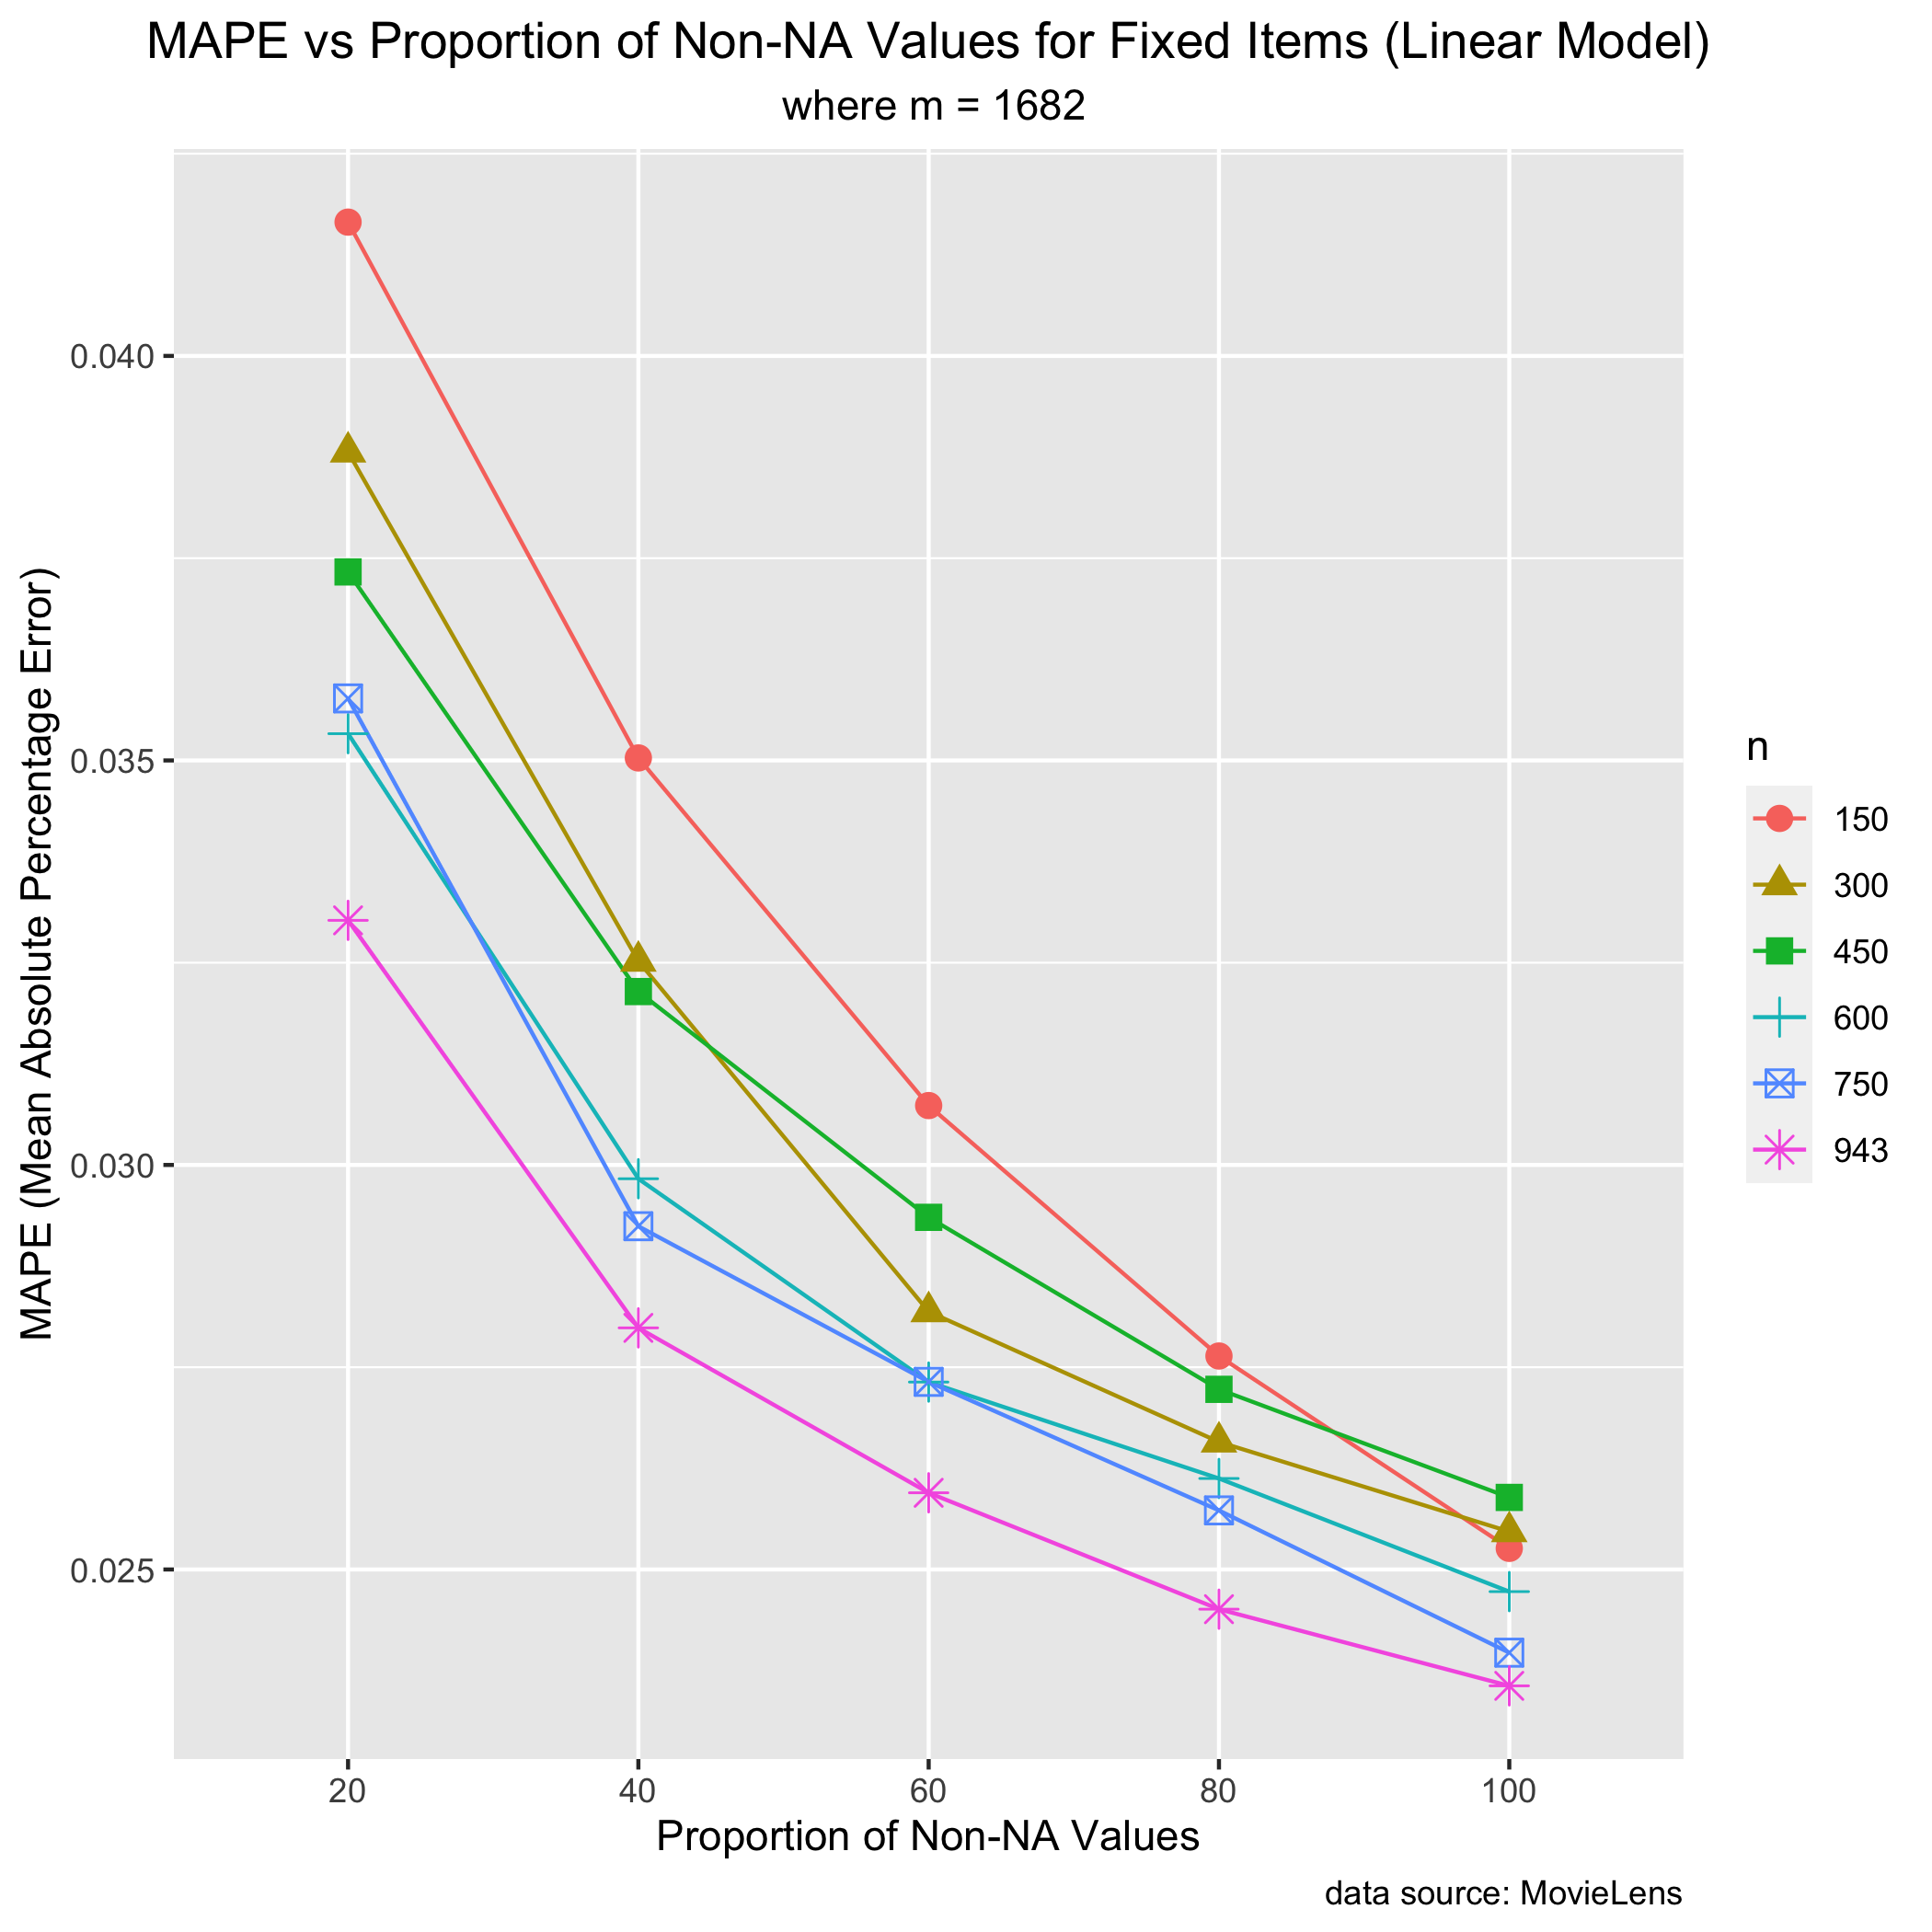
\includegraphics[width=1.2\textwidth]{MovieLens/Linear Model/m-1682 (mape).png}
        \caption{m-1682 (mape)}
        
    \end{minipage}\hfill
    \begin{minipage}{0.45\textwidth}
        \centering
        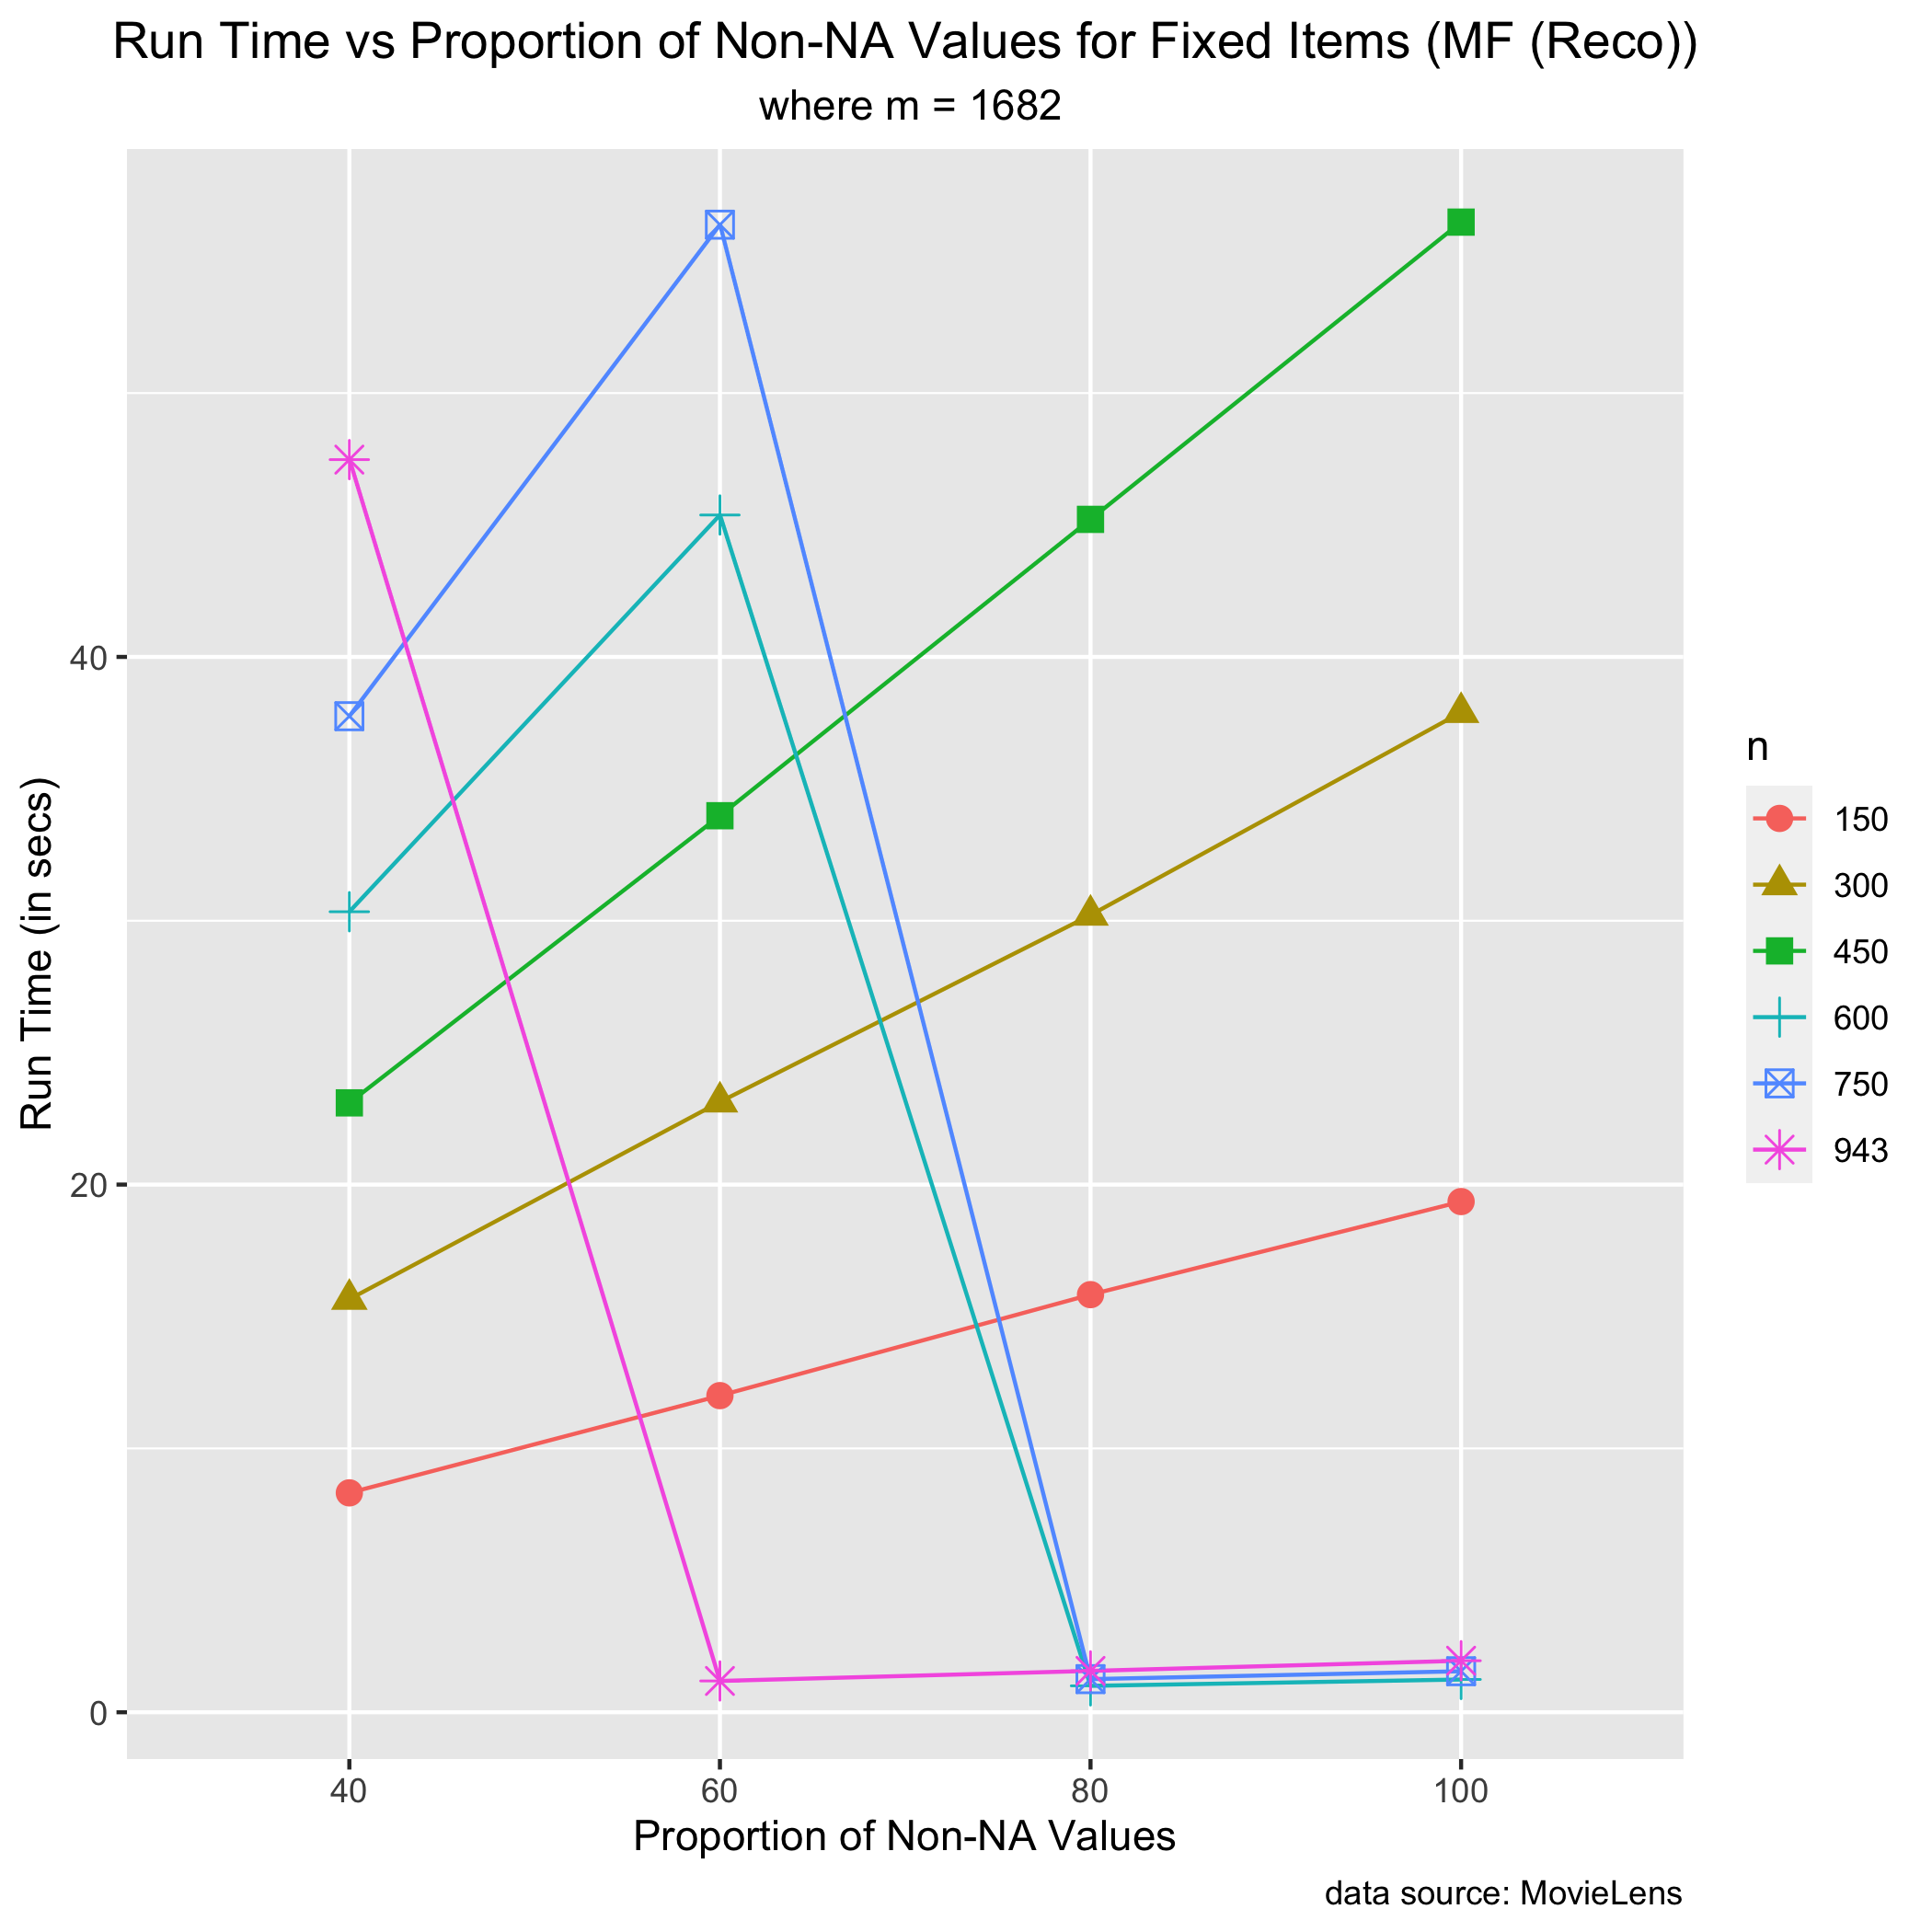
\includegraphics[width=1.2\textwidth]{MovieLens/Linear Model/m-1682 (run time).png}
        \caption{m-1682 (run time)}
    \end{minipage}
\end{figure}

\paragraph{Fixed N}
Compare across curves:\newline
As M increases, curves of MAPE move downward, curves of run time move upward.
\newline
Compare along curves:\newline
As N increases, MAPE decreases and run time increases. 

% figure n=150
\begin{figure}[H]
\centering
    \begin{minipage}{0.45\textwidth}
        \centering
        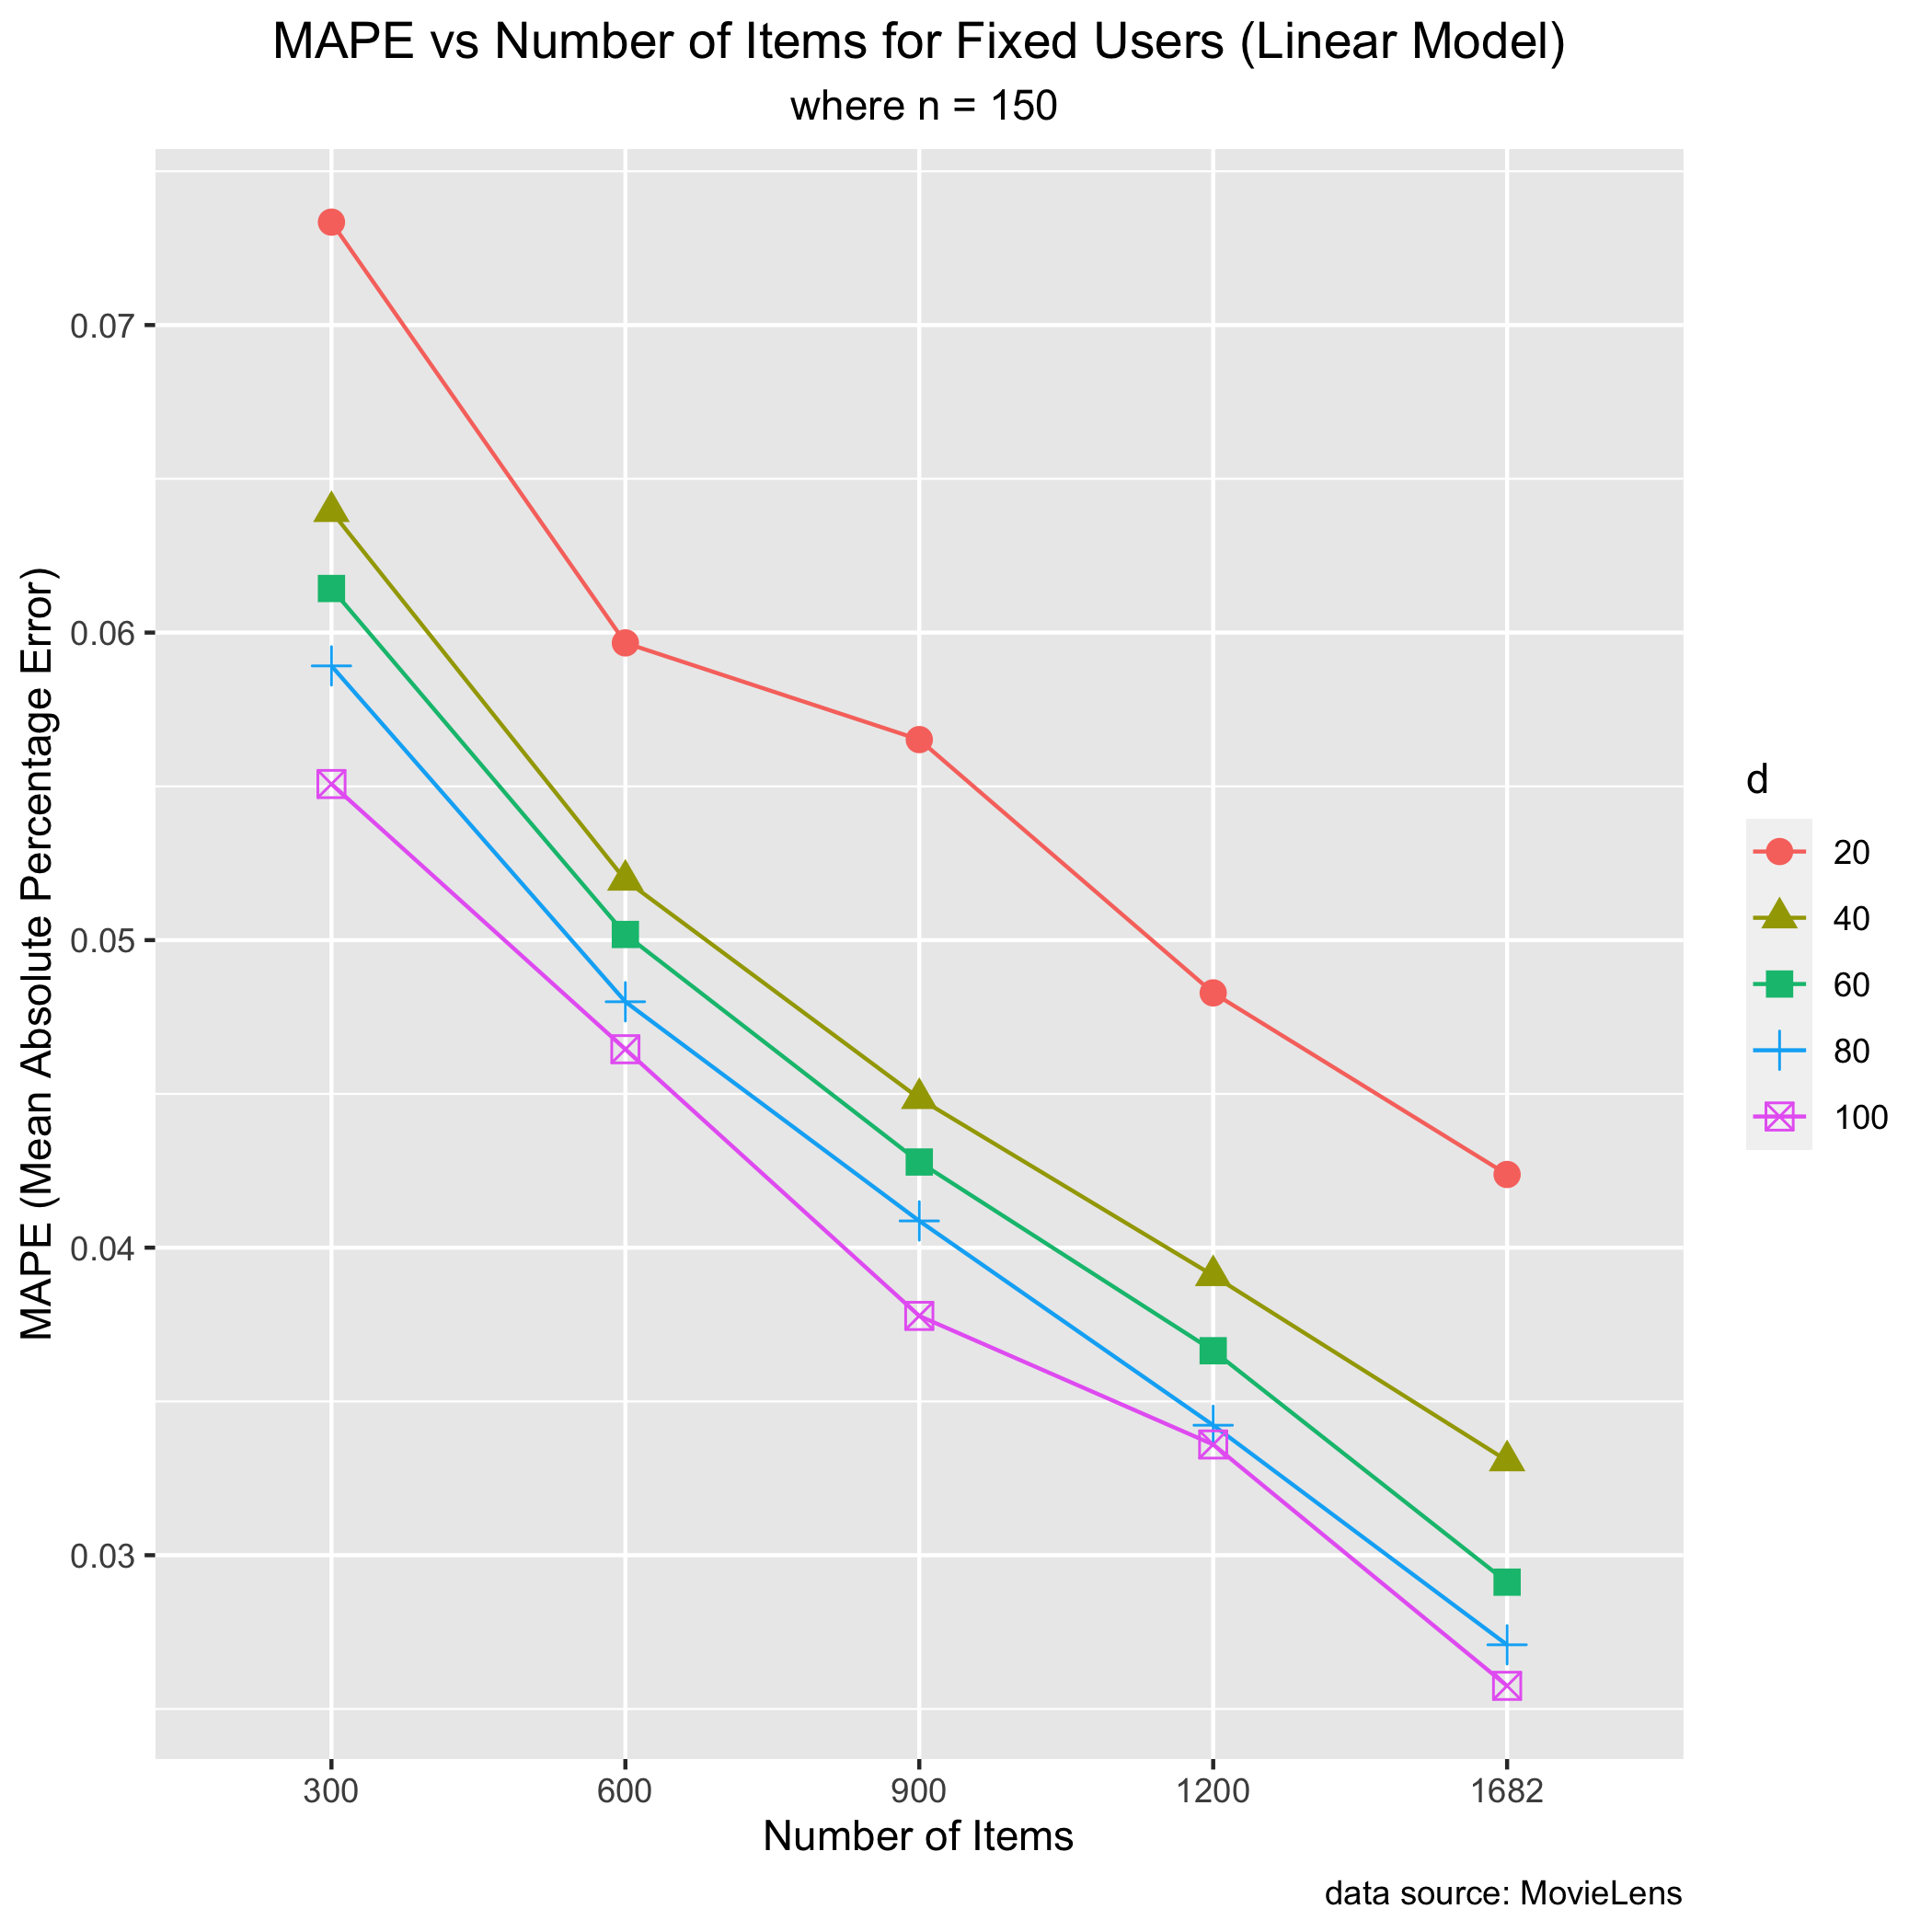
\includegraphics[width=1.2\textwidth]{MovieLens/Linear Model/n-150 (mape).png}
        \caption{n-150 (mape)}
        
    \end{minipage}\hfill
    \begin{minipage}{0.45\textwidth}
        \centering
        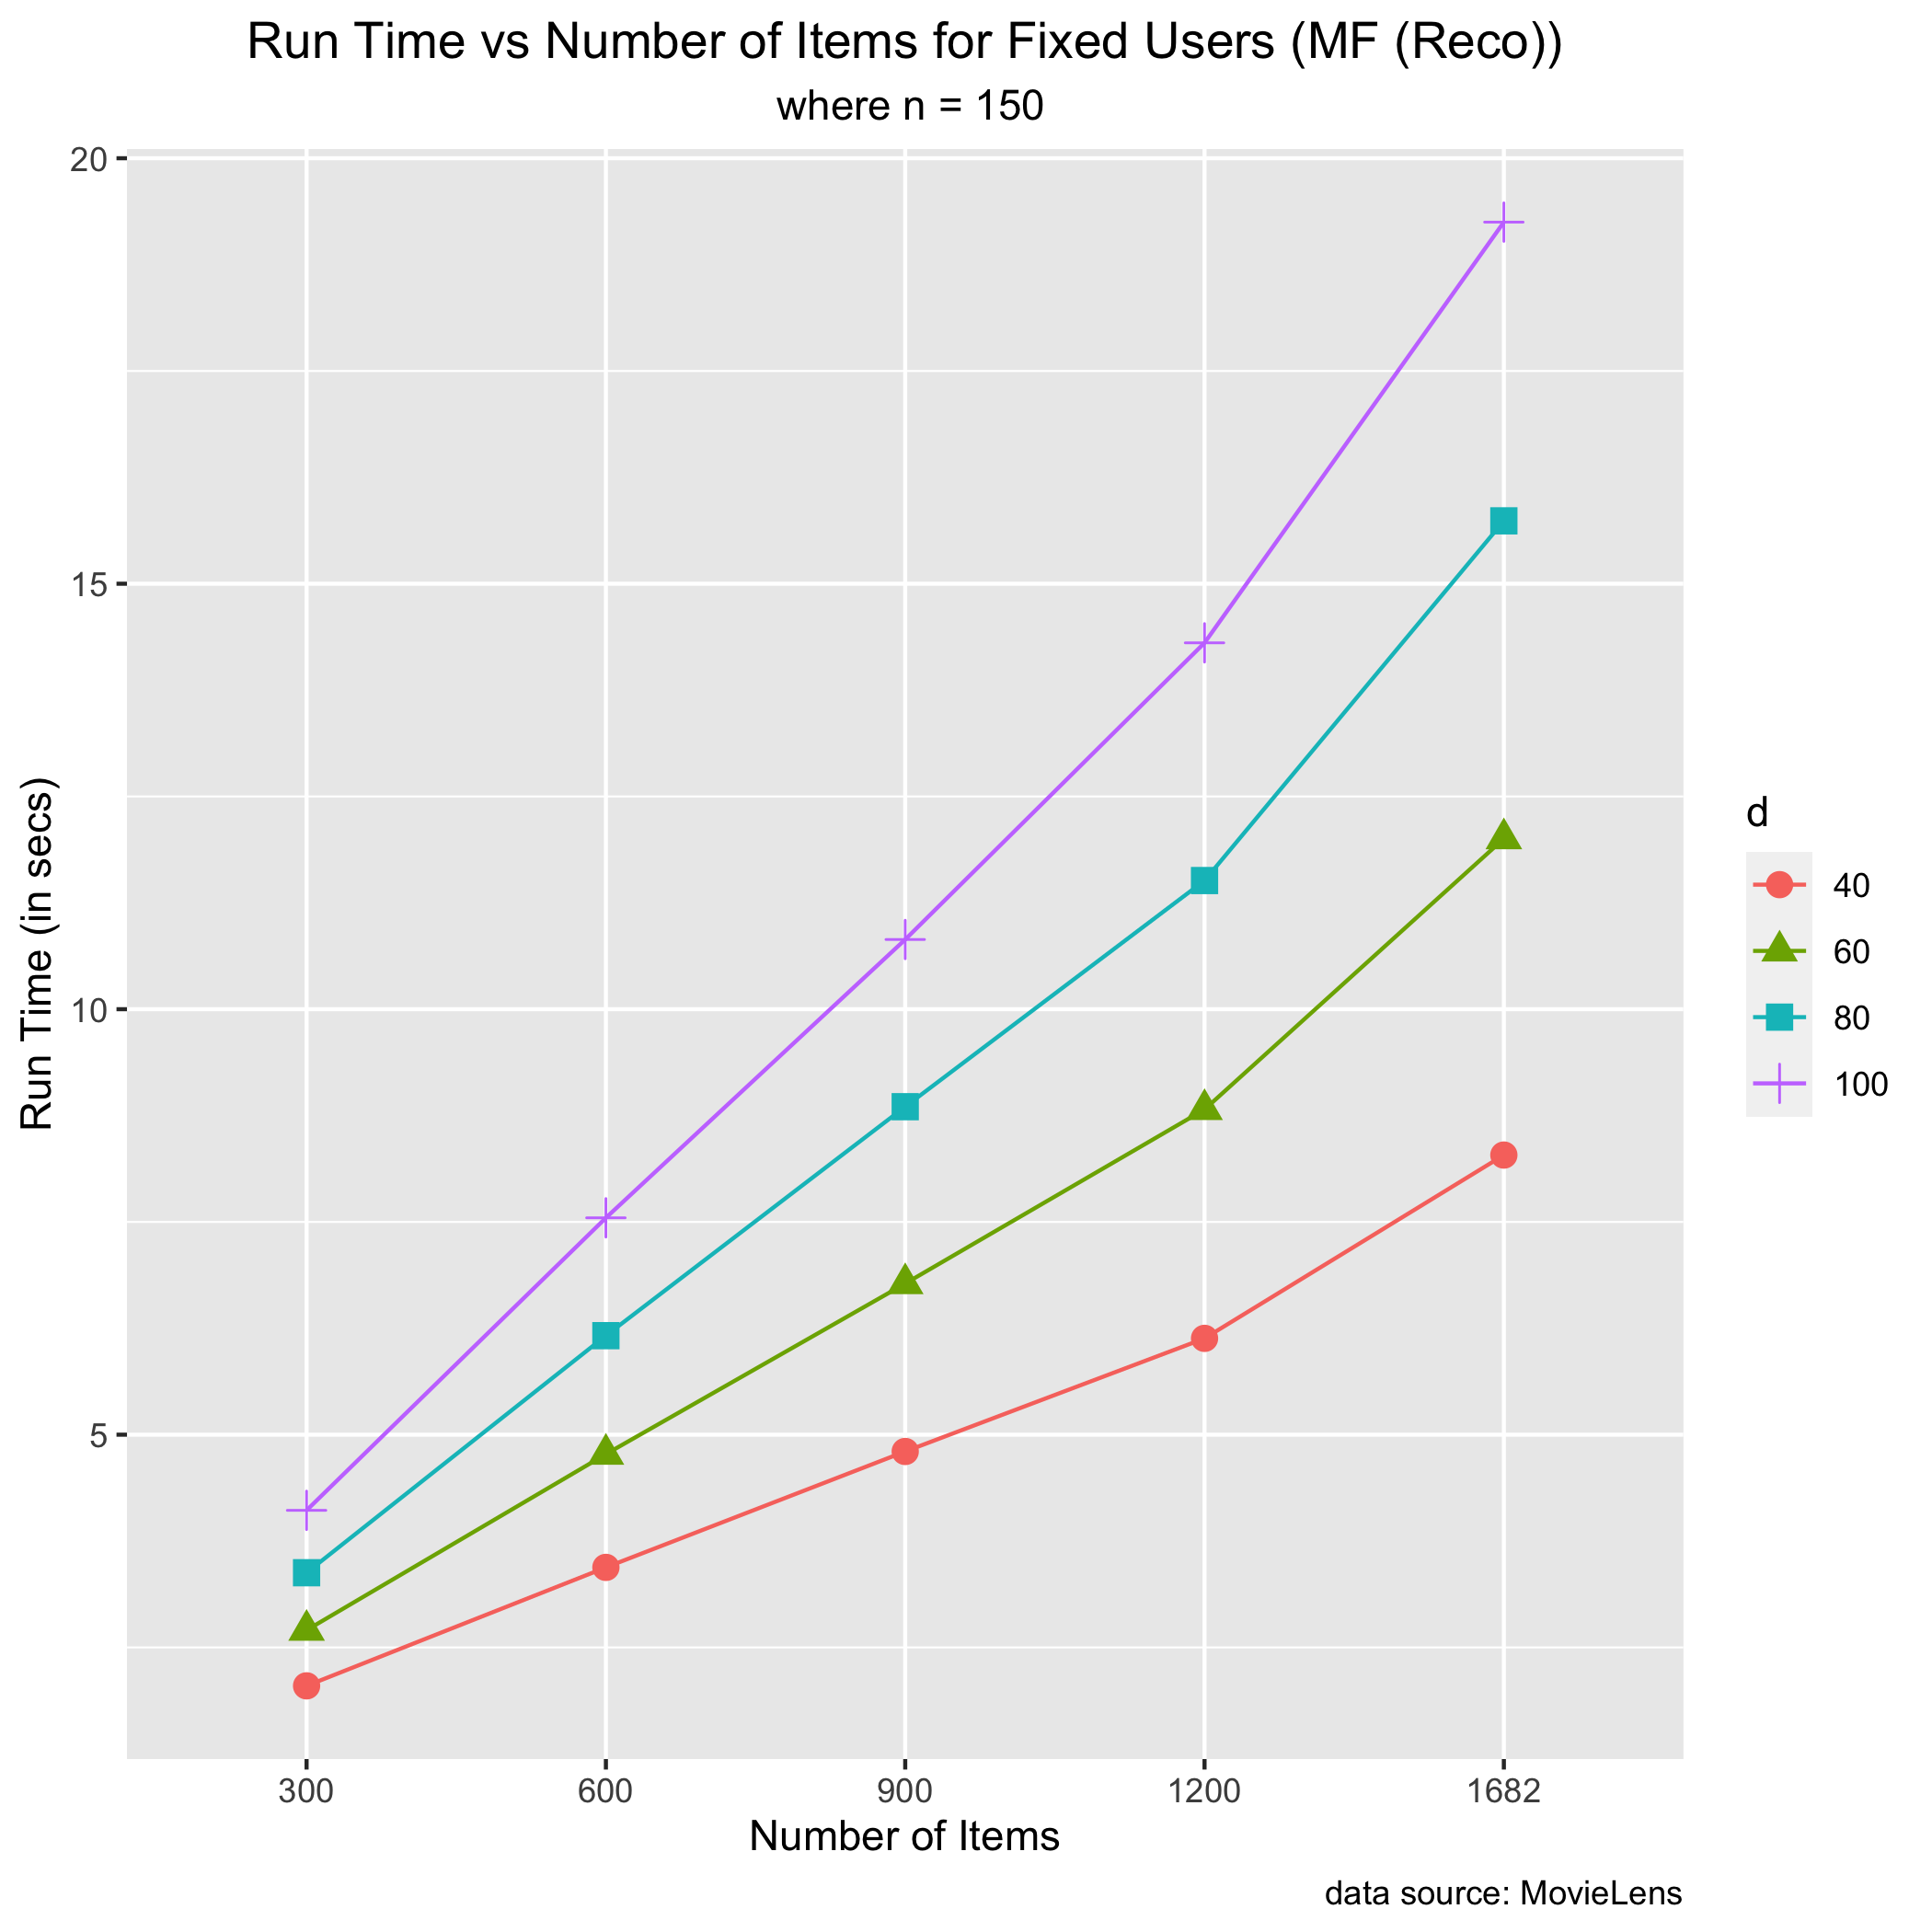
\includegraphics[width=1.2\textwidth]{MovieLens/Linear Model/n-150 (run time).png}
        \caption{n-150 (run time)}
    \end{minipage}
\end{figure}

% figure n=300
\begin{figure}[H]
\centering
    \begin{minipage}{0.45\textwidth}
        \centering
        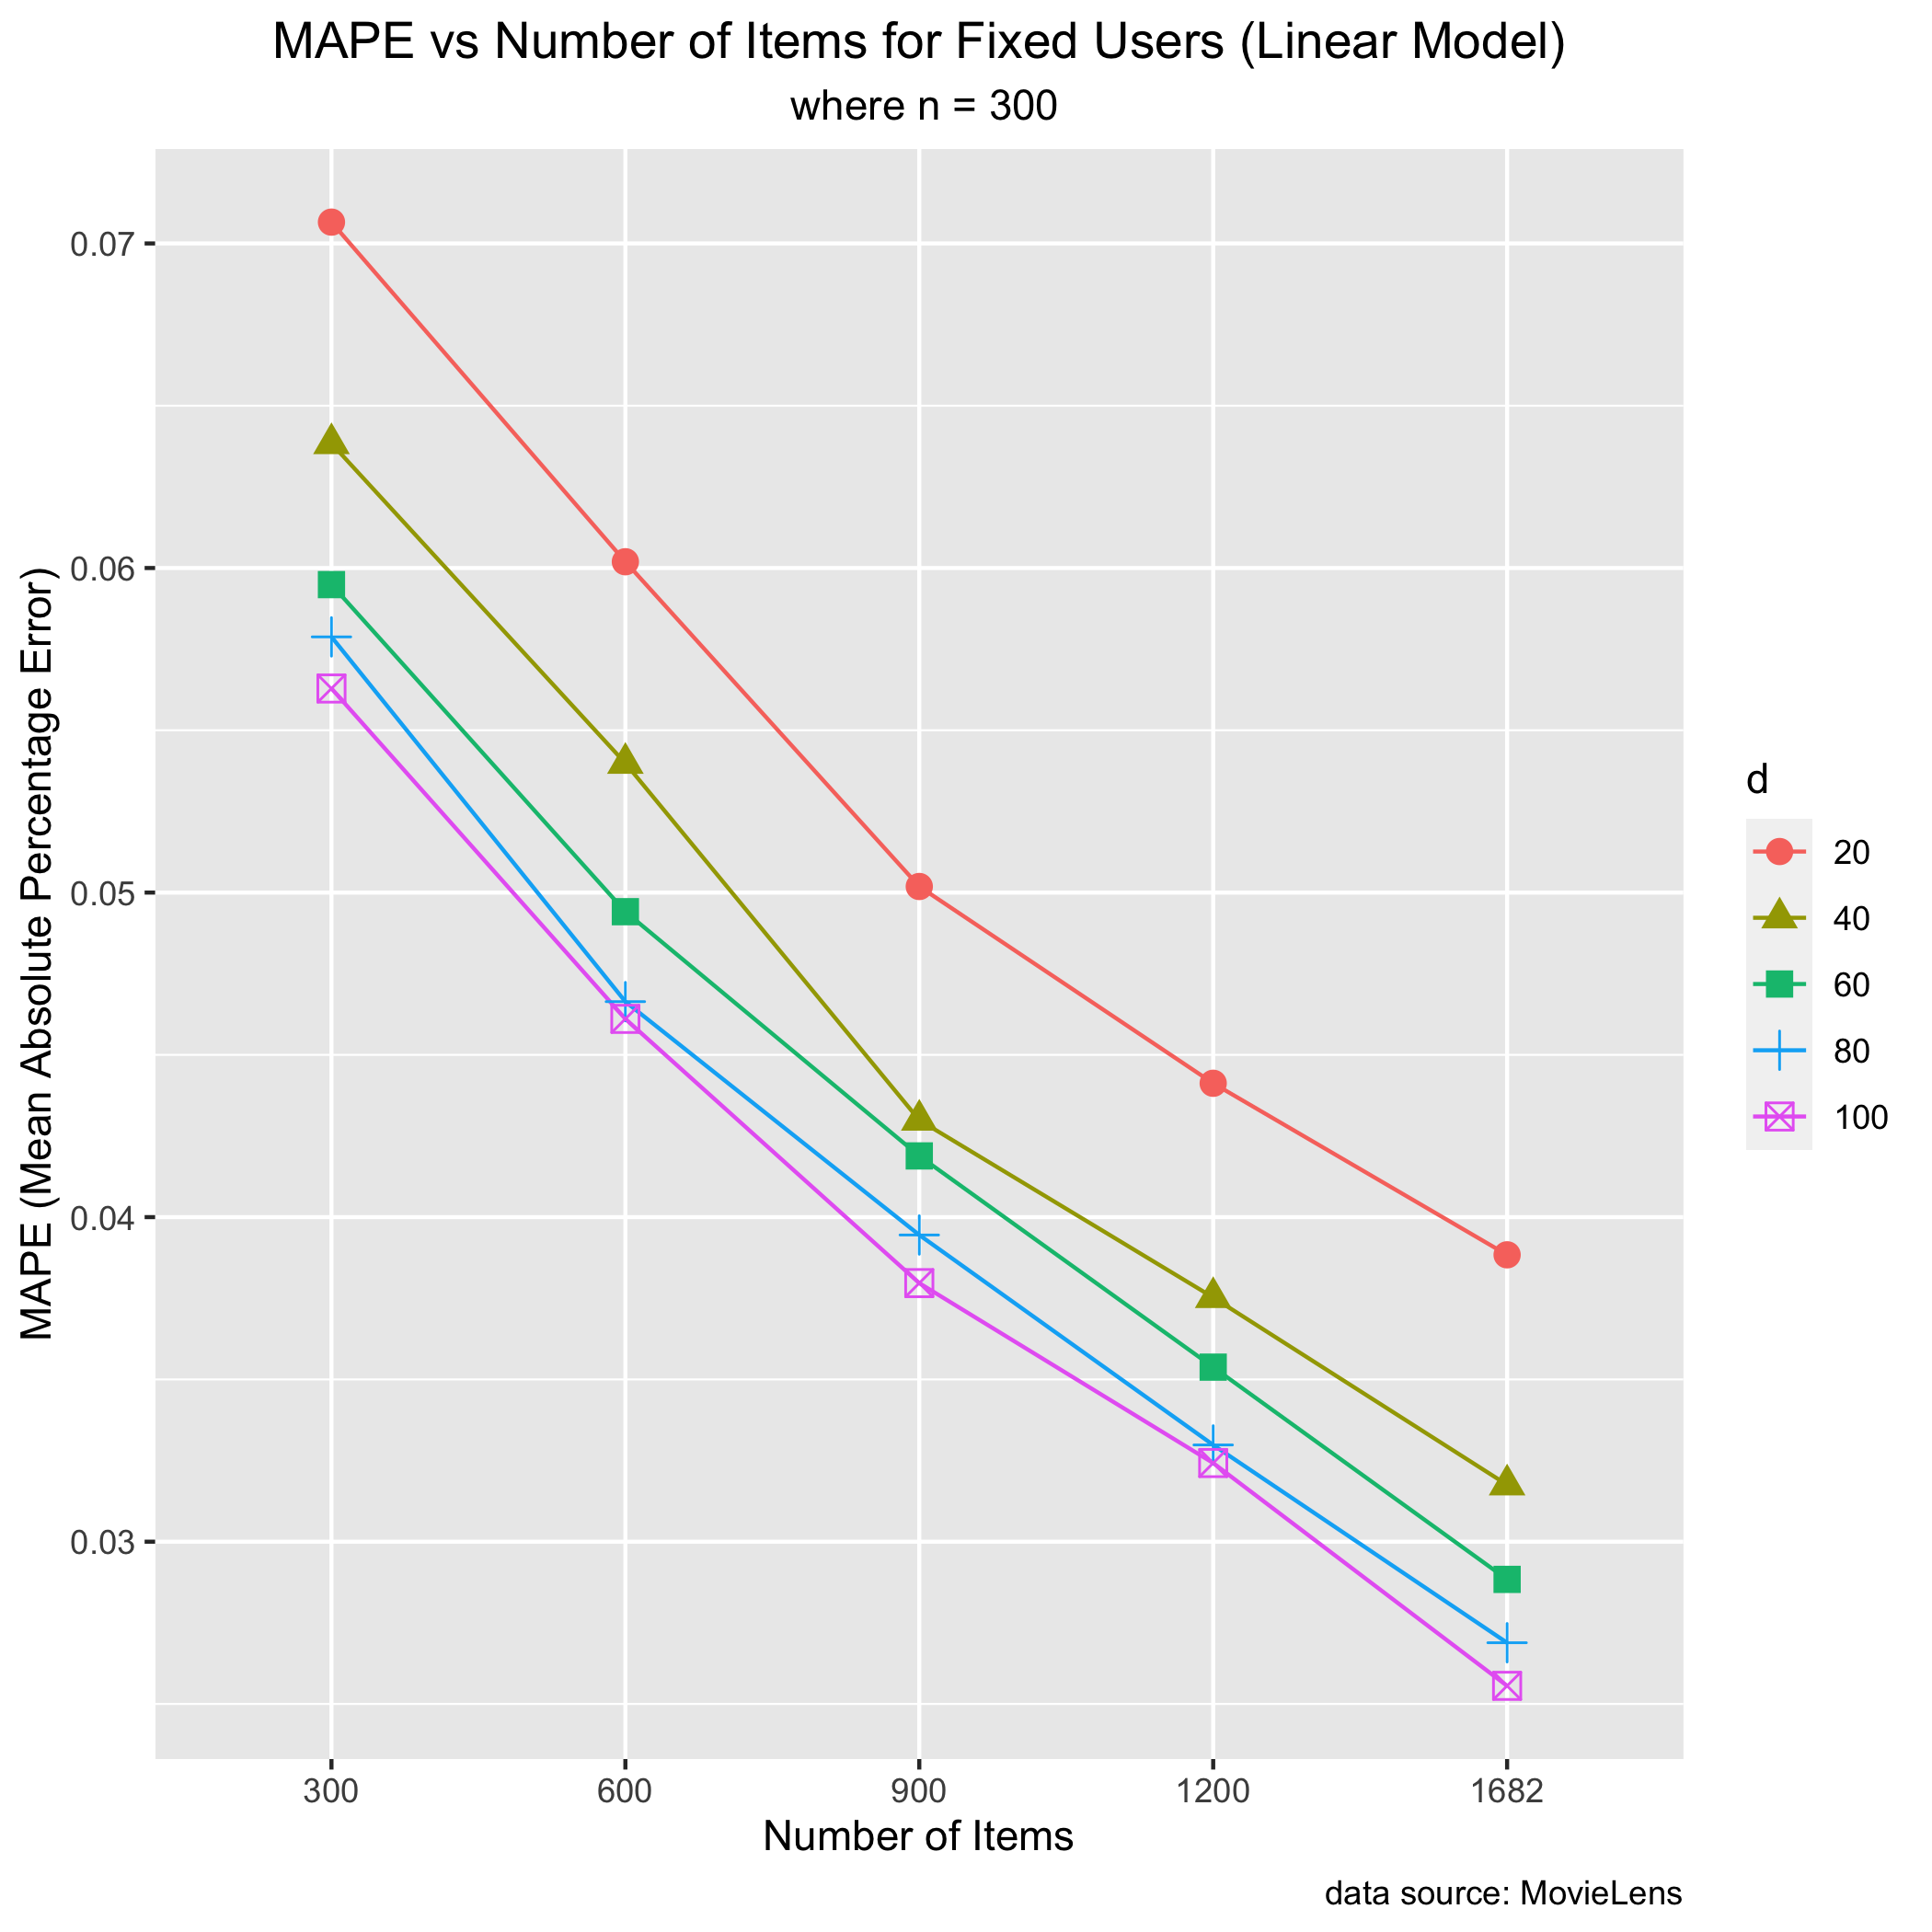
\includegraphics[width=1.2\textwidth]{MovieLens/Linear Model/n-300 (mape).png}
        \caption{n-300 (mape)}
        
    \end{minipage}\hfill
    \begin{minipage}{0.45\textwidth}
        \centering
        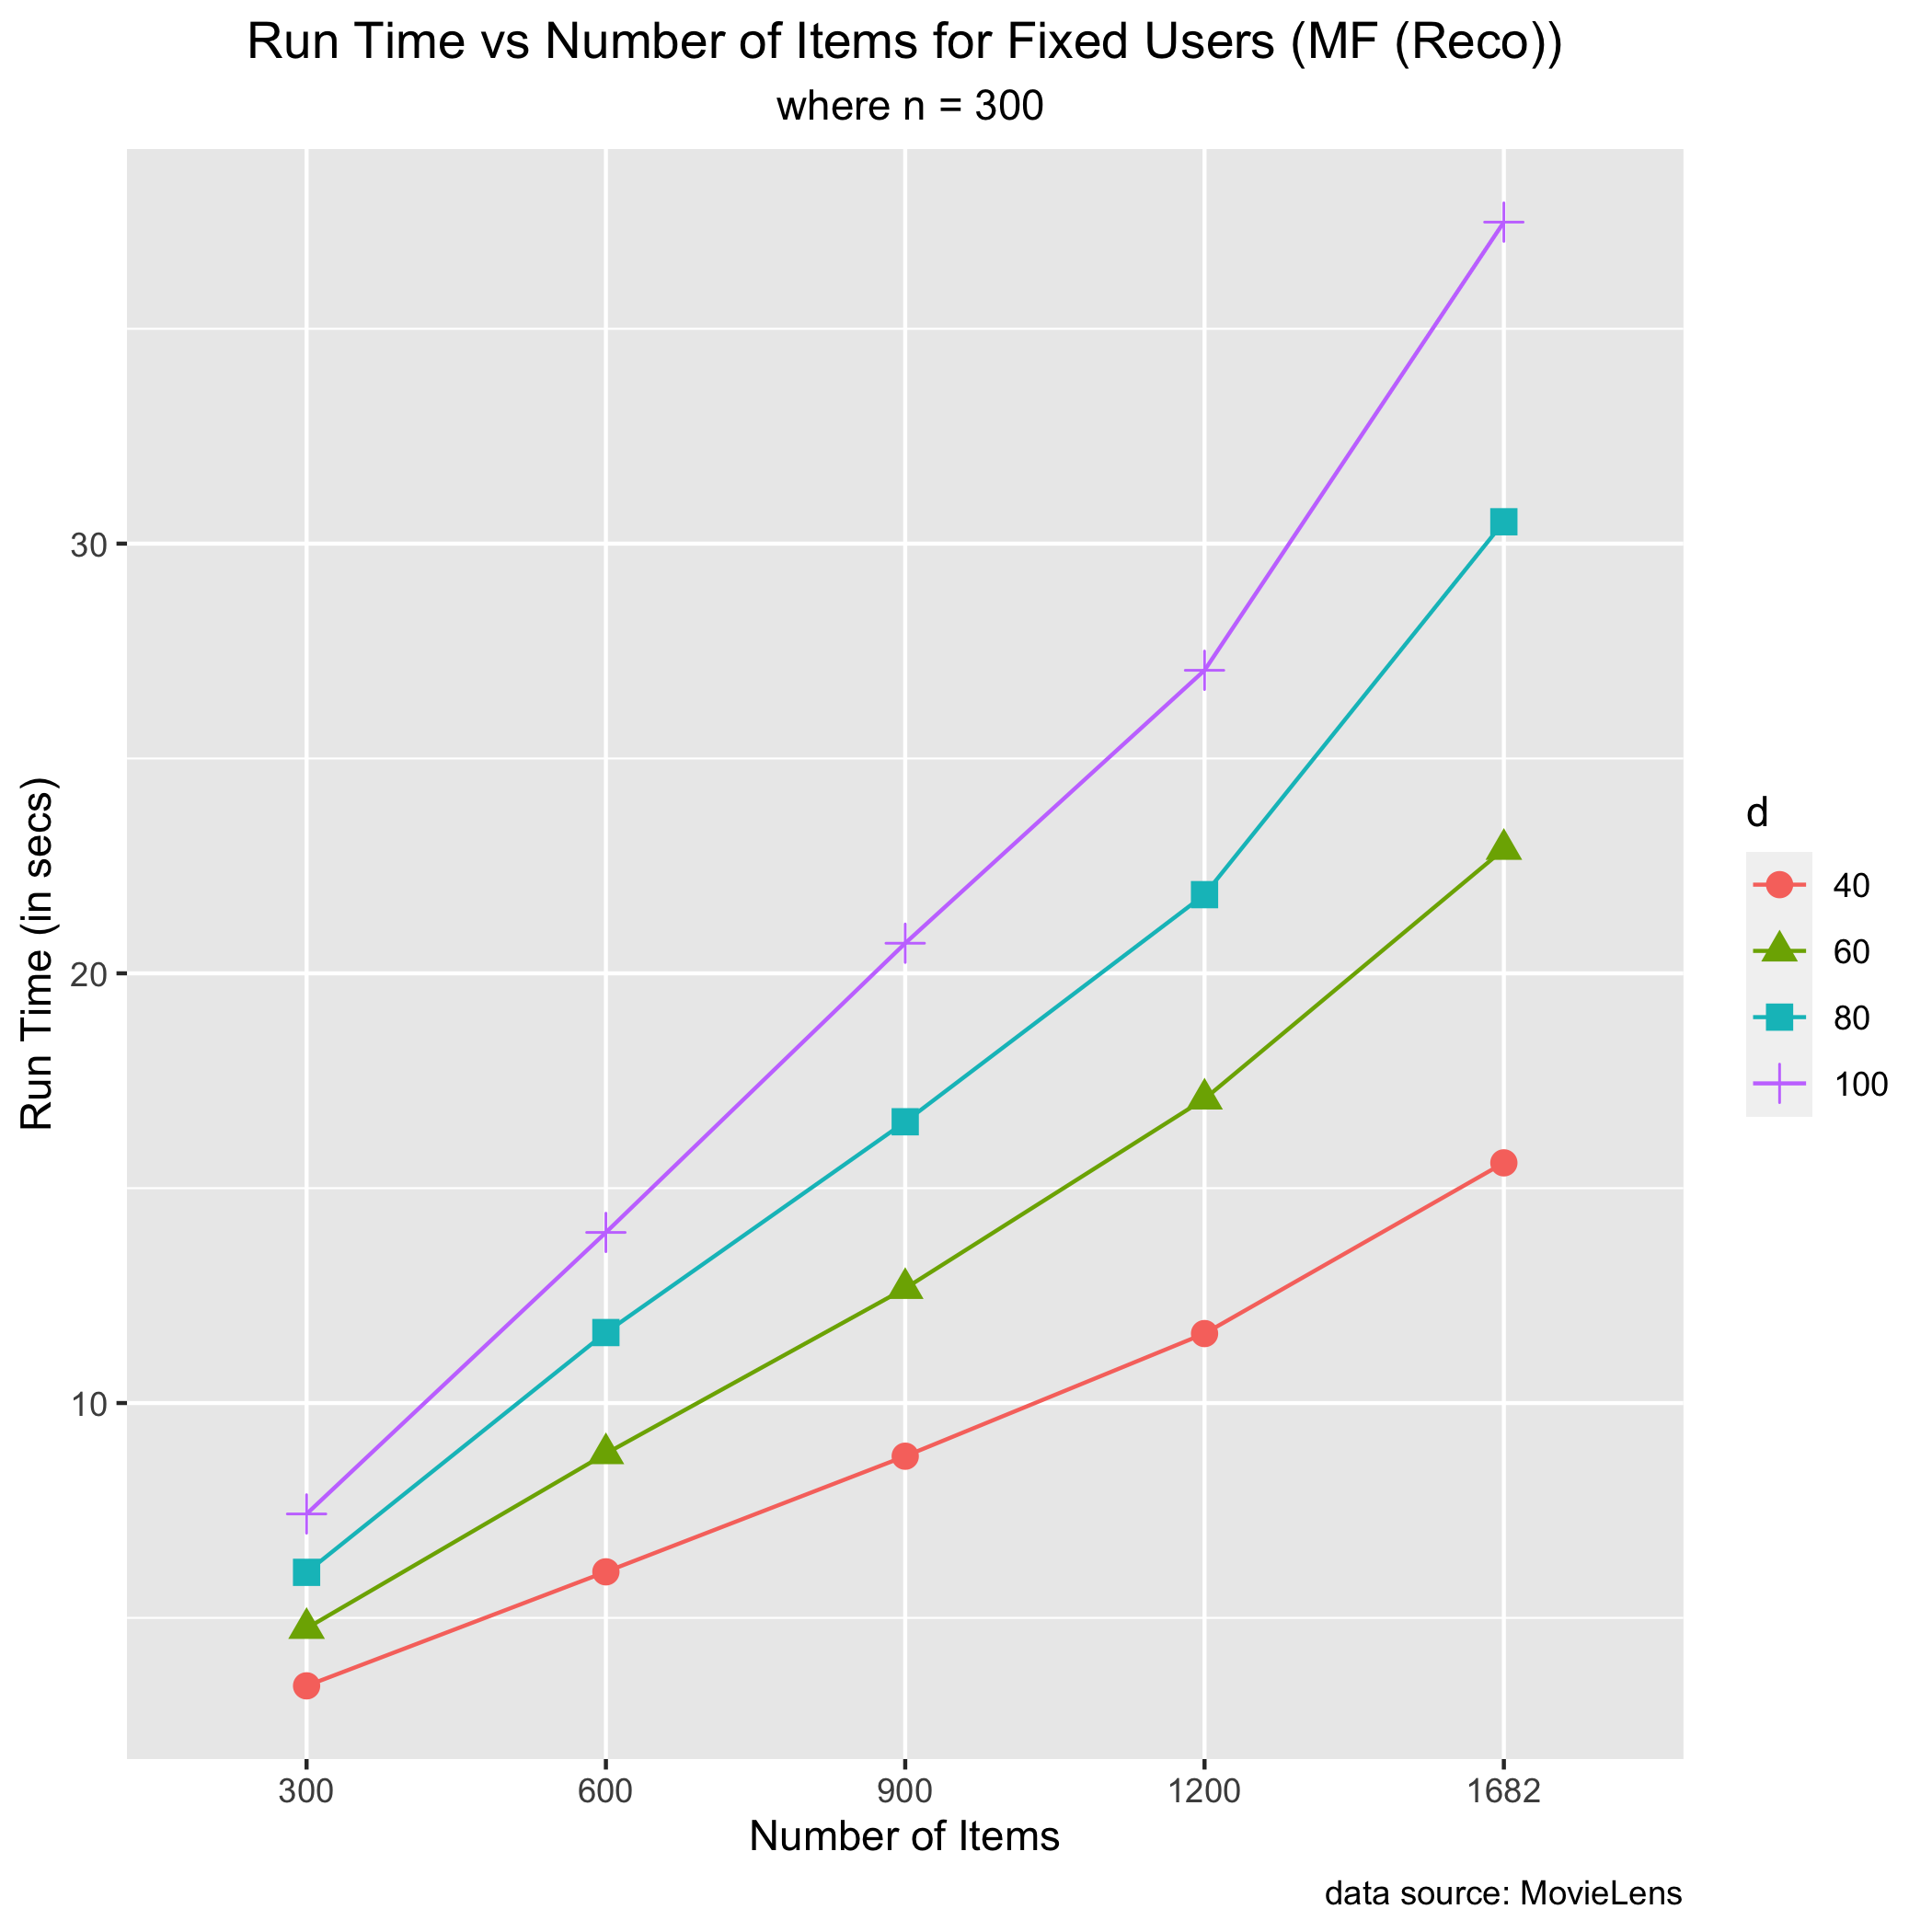
\includegraphics[width=1.2\textwidth]{MovieLens/Linear Model/n-300 (run time).png}
        \caption{n-300 (run time)}
    \end{minipage}
\end{figure}

% figure n=450
\begin{figure}[H]
\centering
    \begin{minipage}{0.45\textwidth}
        \centering
        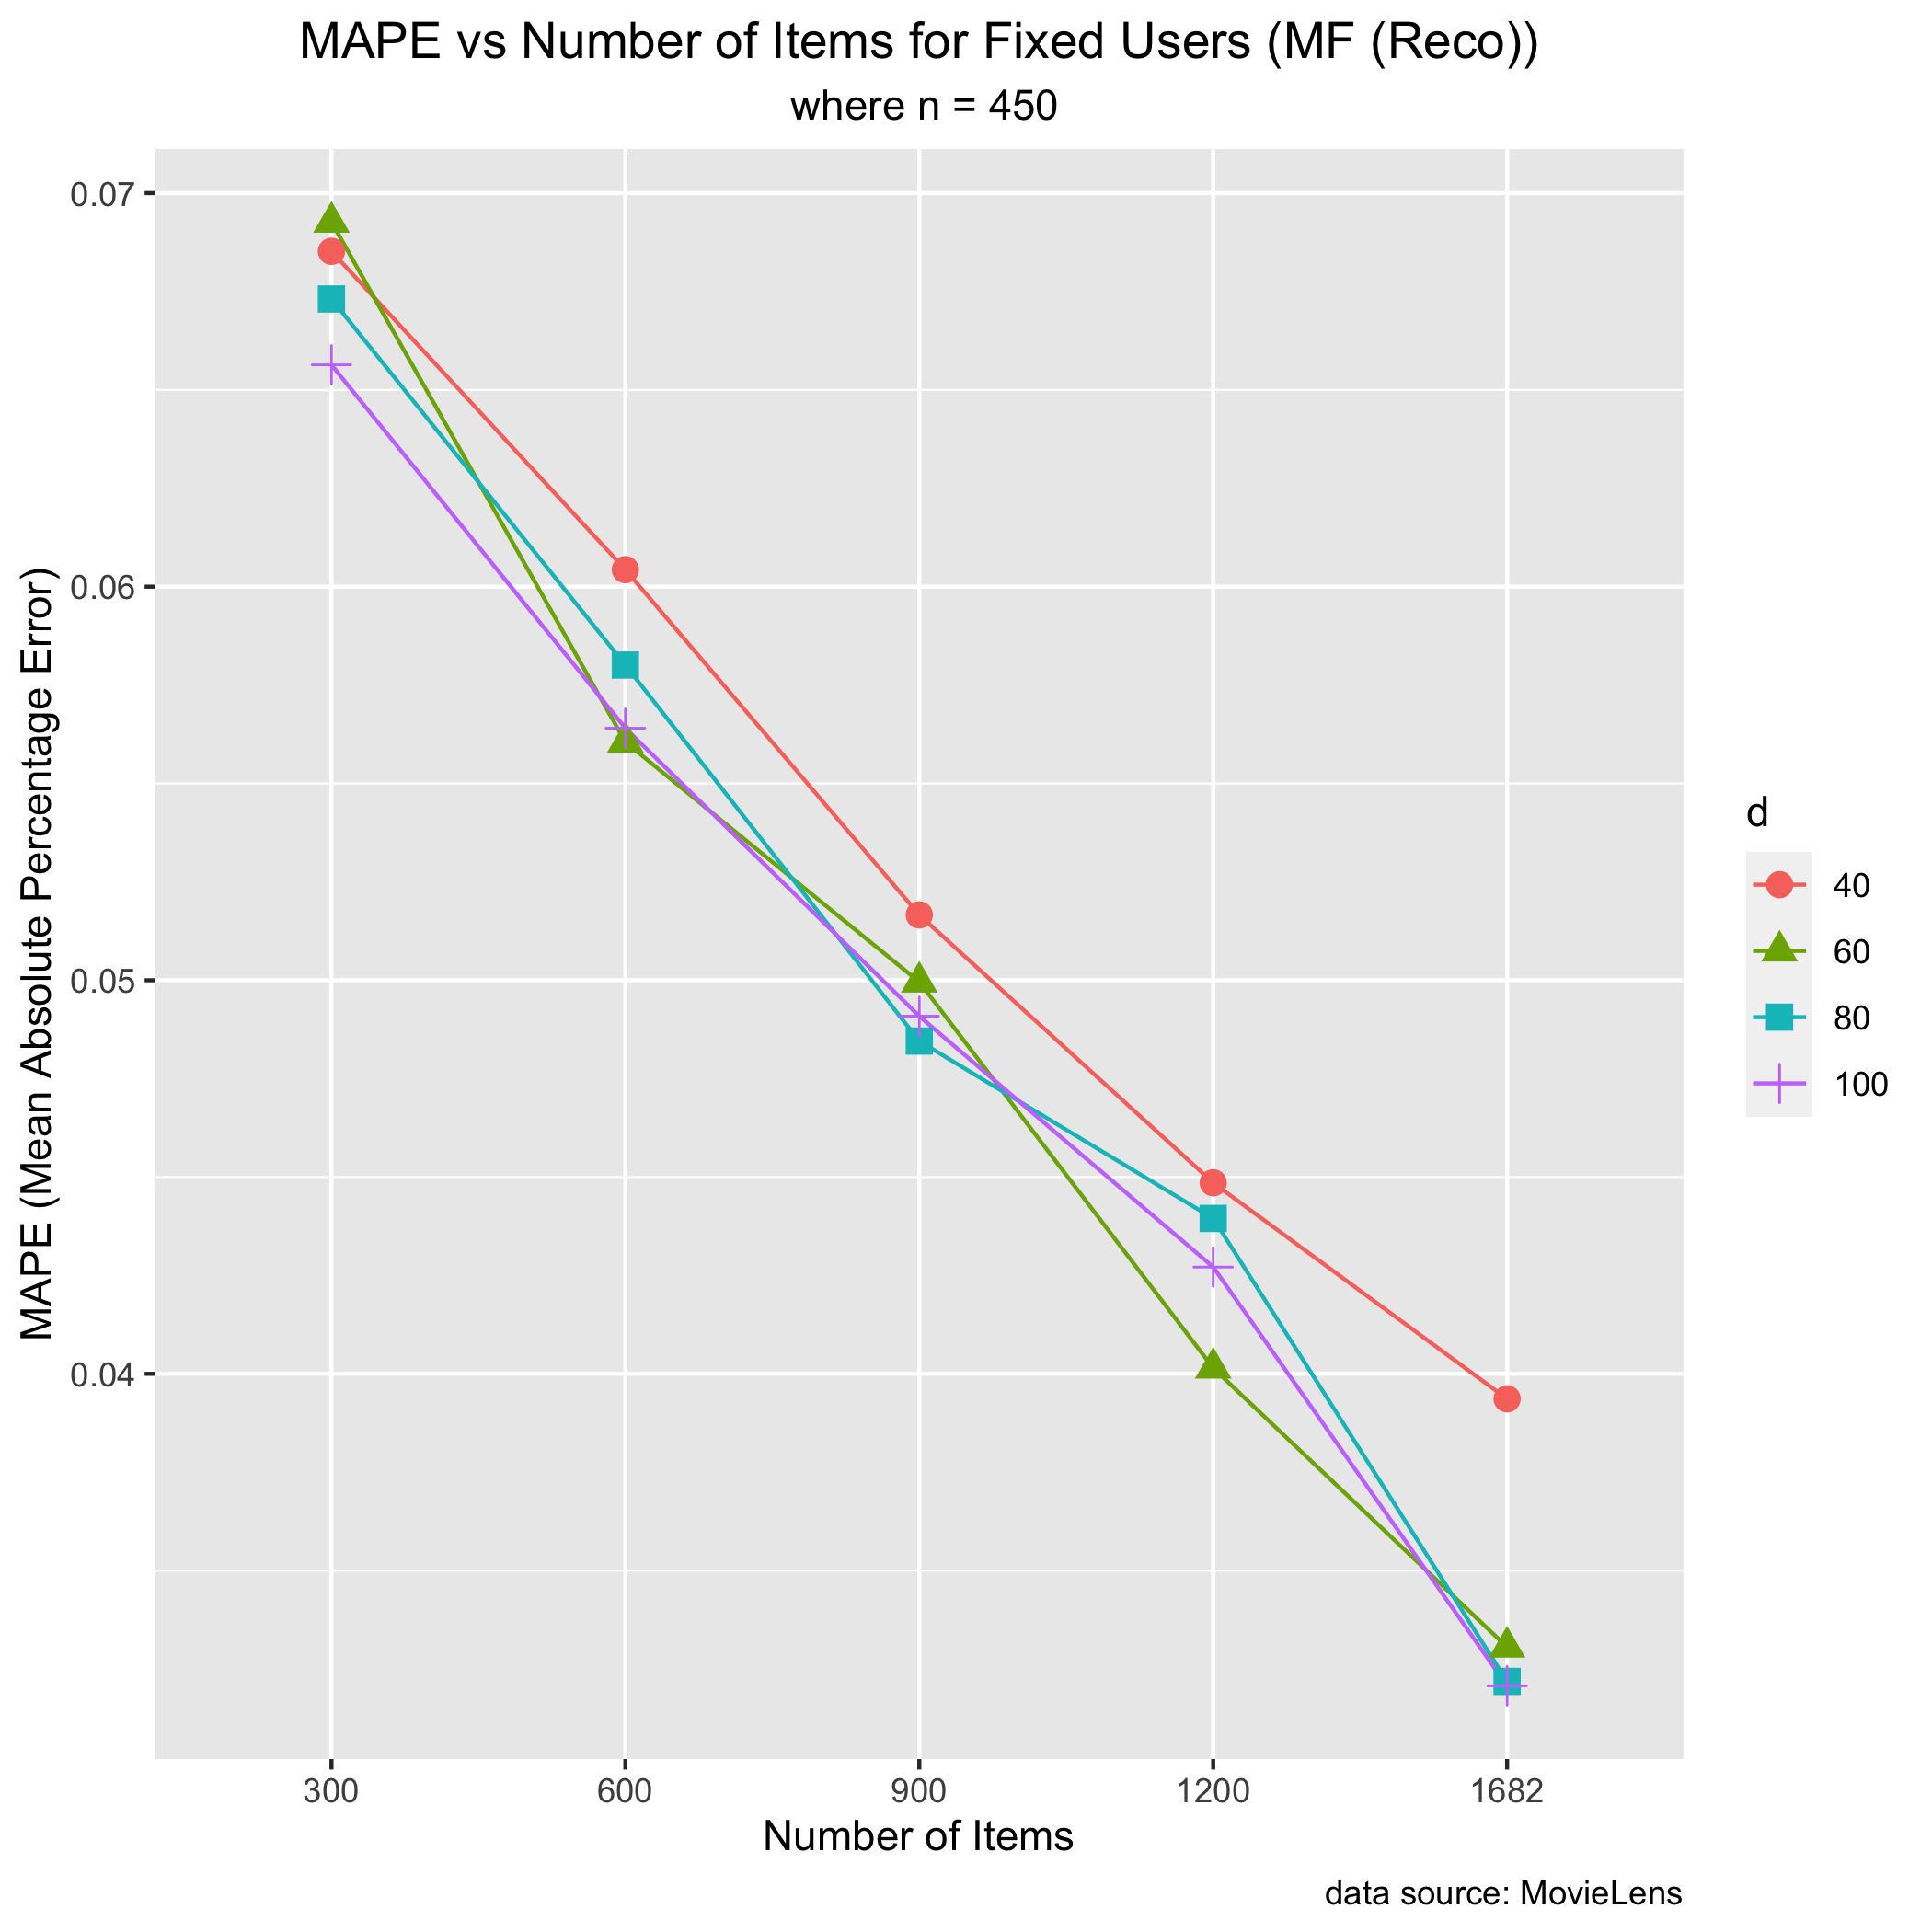
\includegraphics[width=1.2\textwidth]{MovieLens/Linear Model/n-450 (mape).png}
        \caption{n-450 (mape)}
        
    \end{minipage}\hfill
    \begin{minipage}{0.45\textwidth}
        \centering
        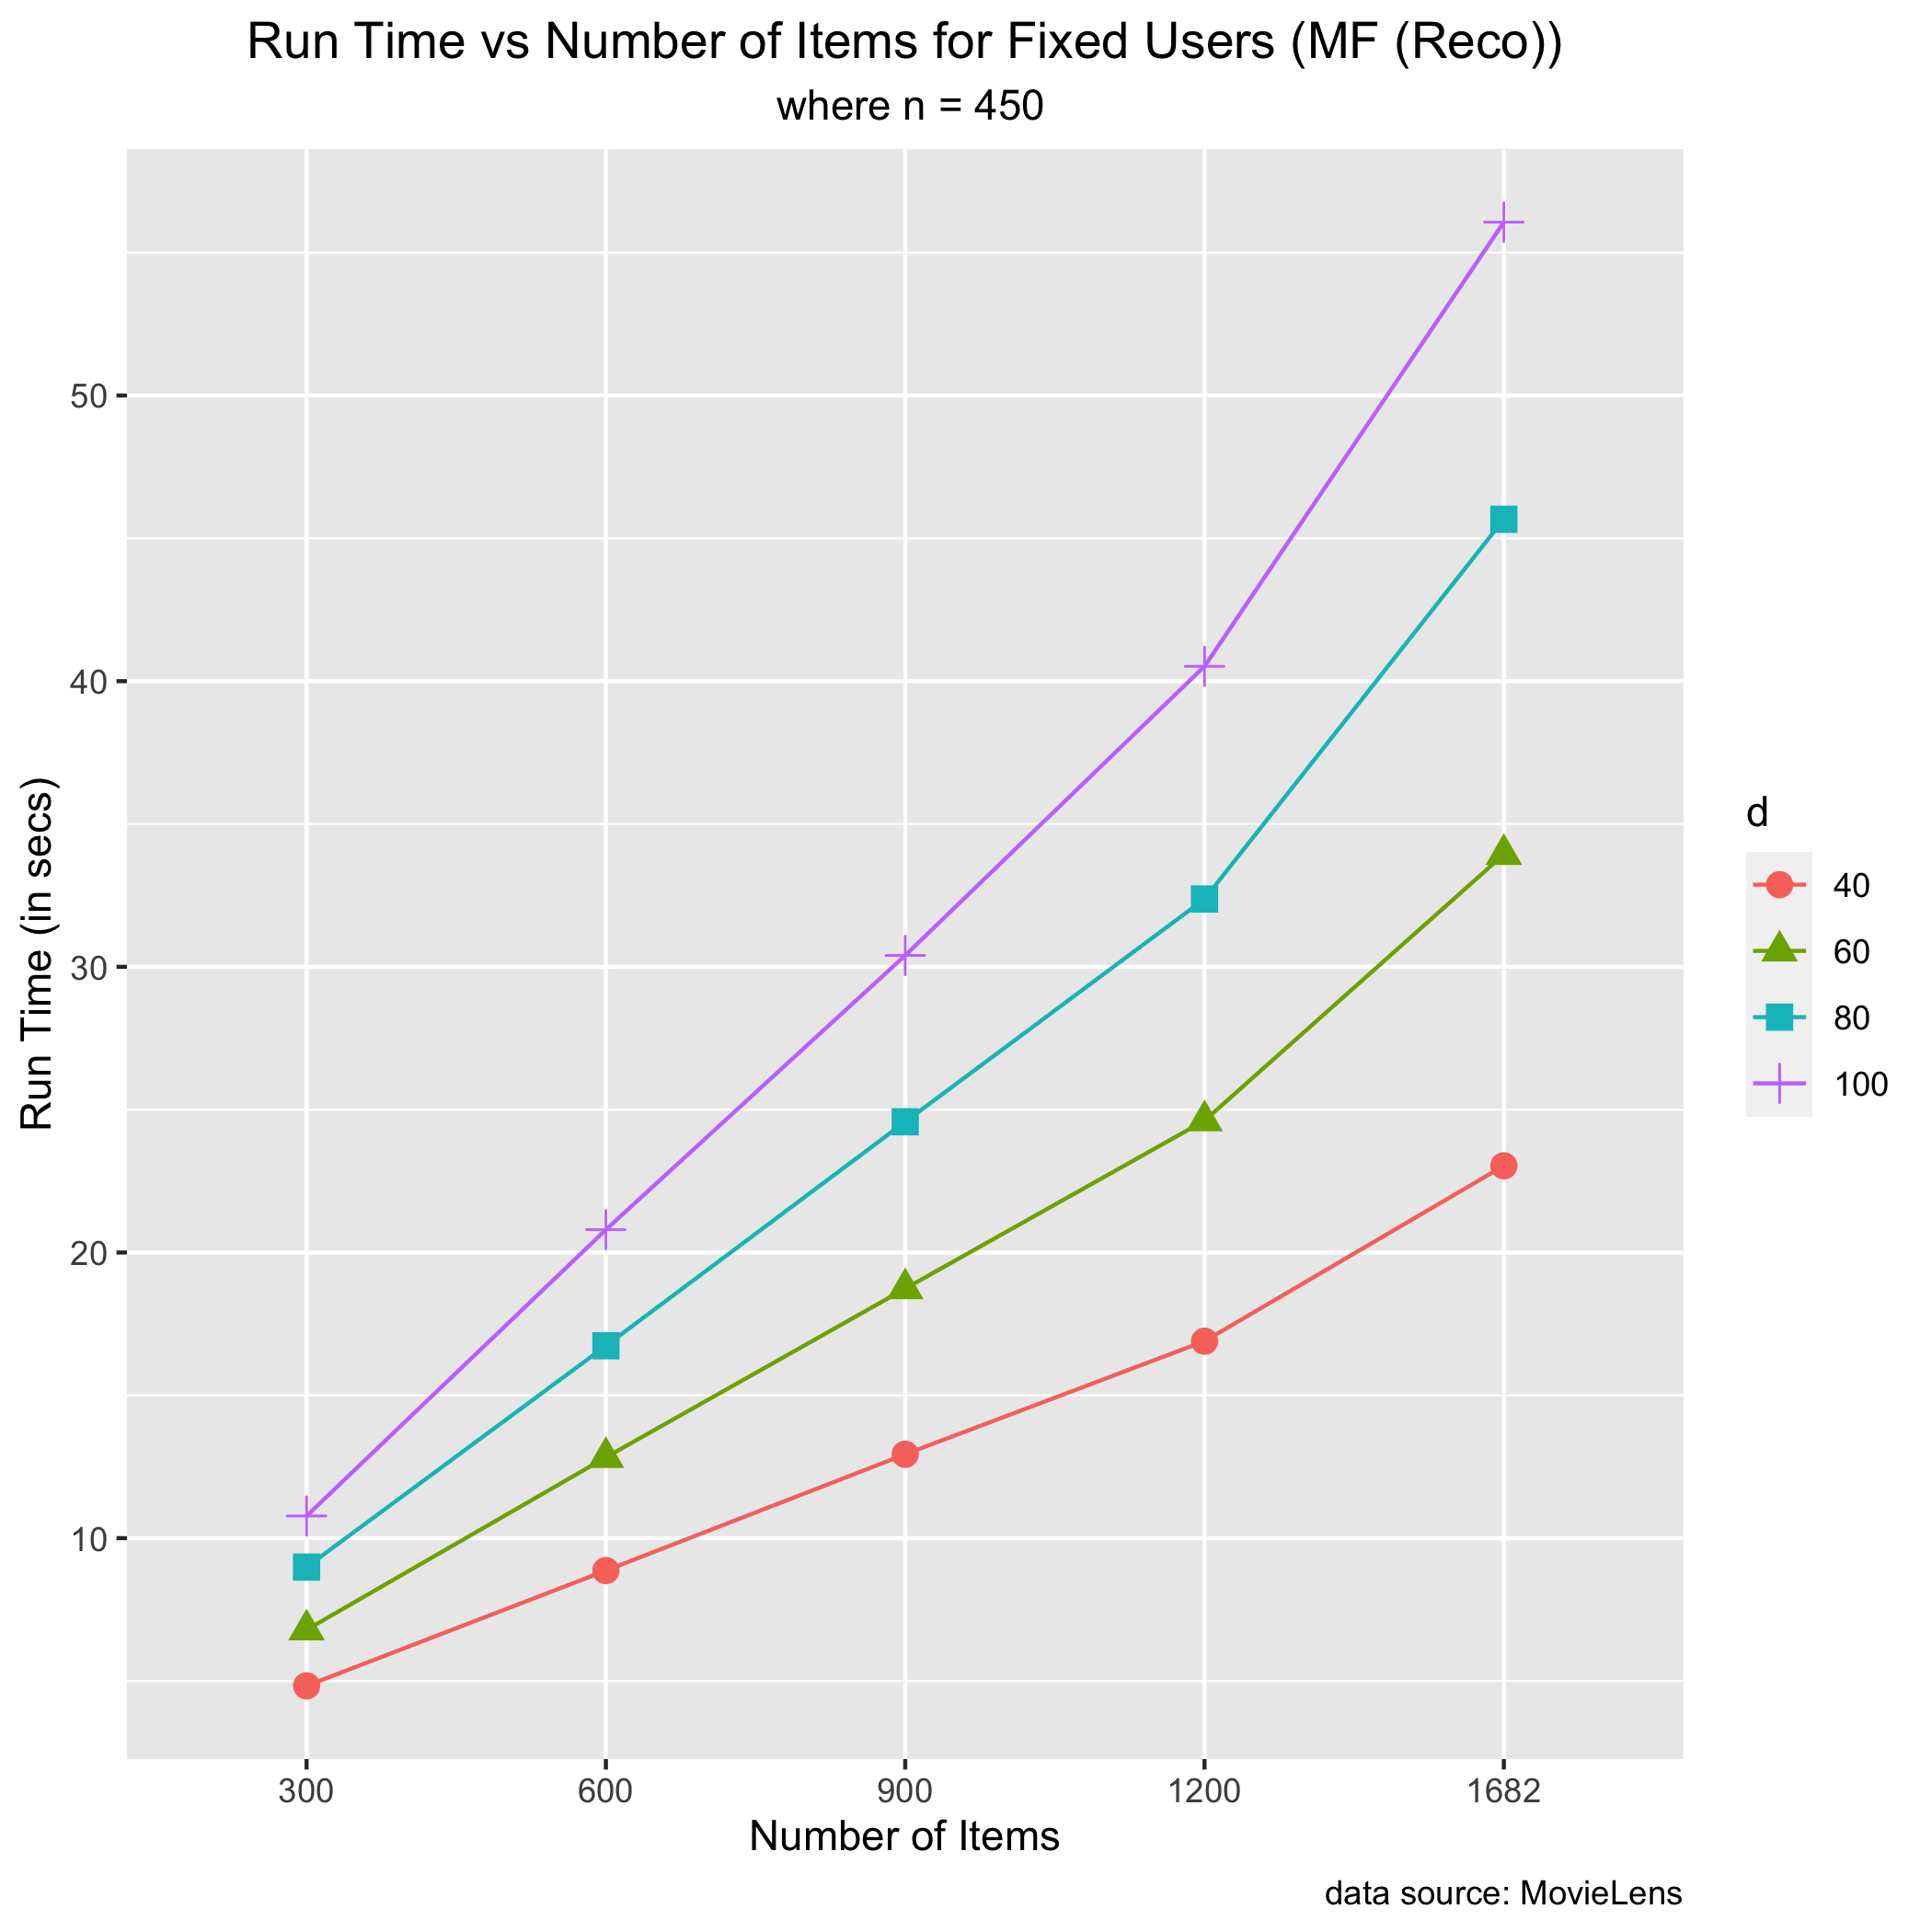
\includegraphics[width=1.2\textwidth]{MovieLens/Linear Model/n-450 (run time).png}
        \caption{n-450 (run time)}
    \end{minipage}
\end{figure}

% figure n=600
\begin{figure}[H]
\centering
    \begin{minipage}{0.45\textwidth}
        \centering
        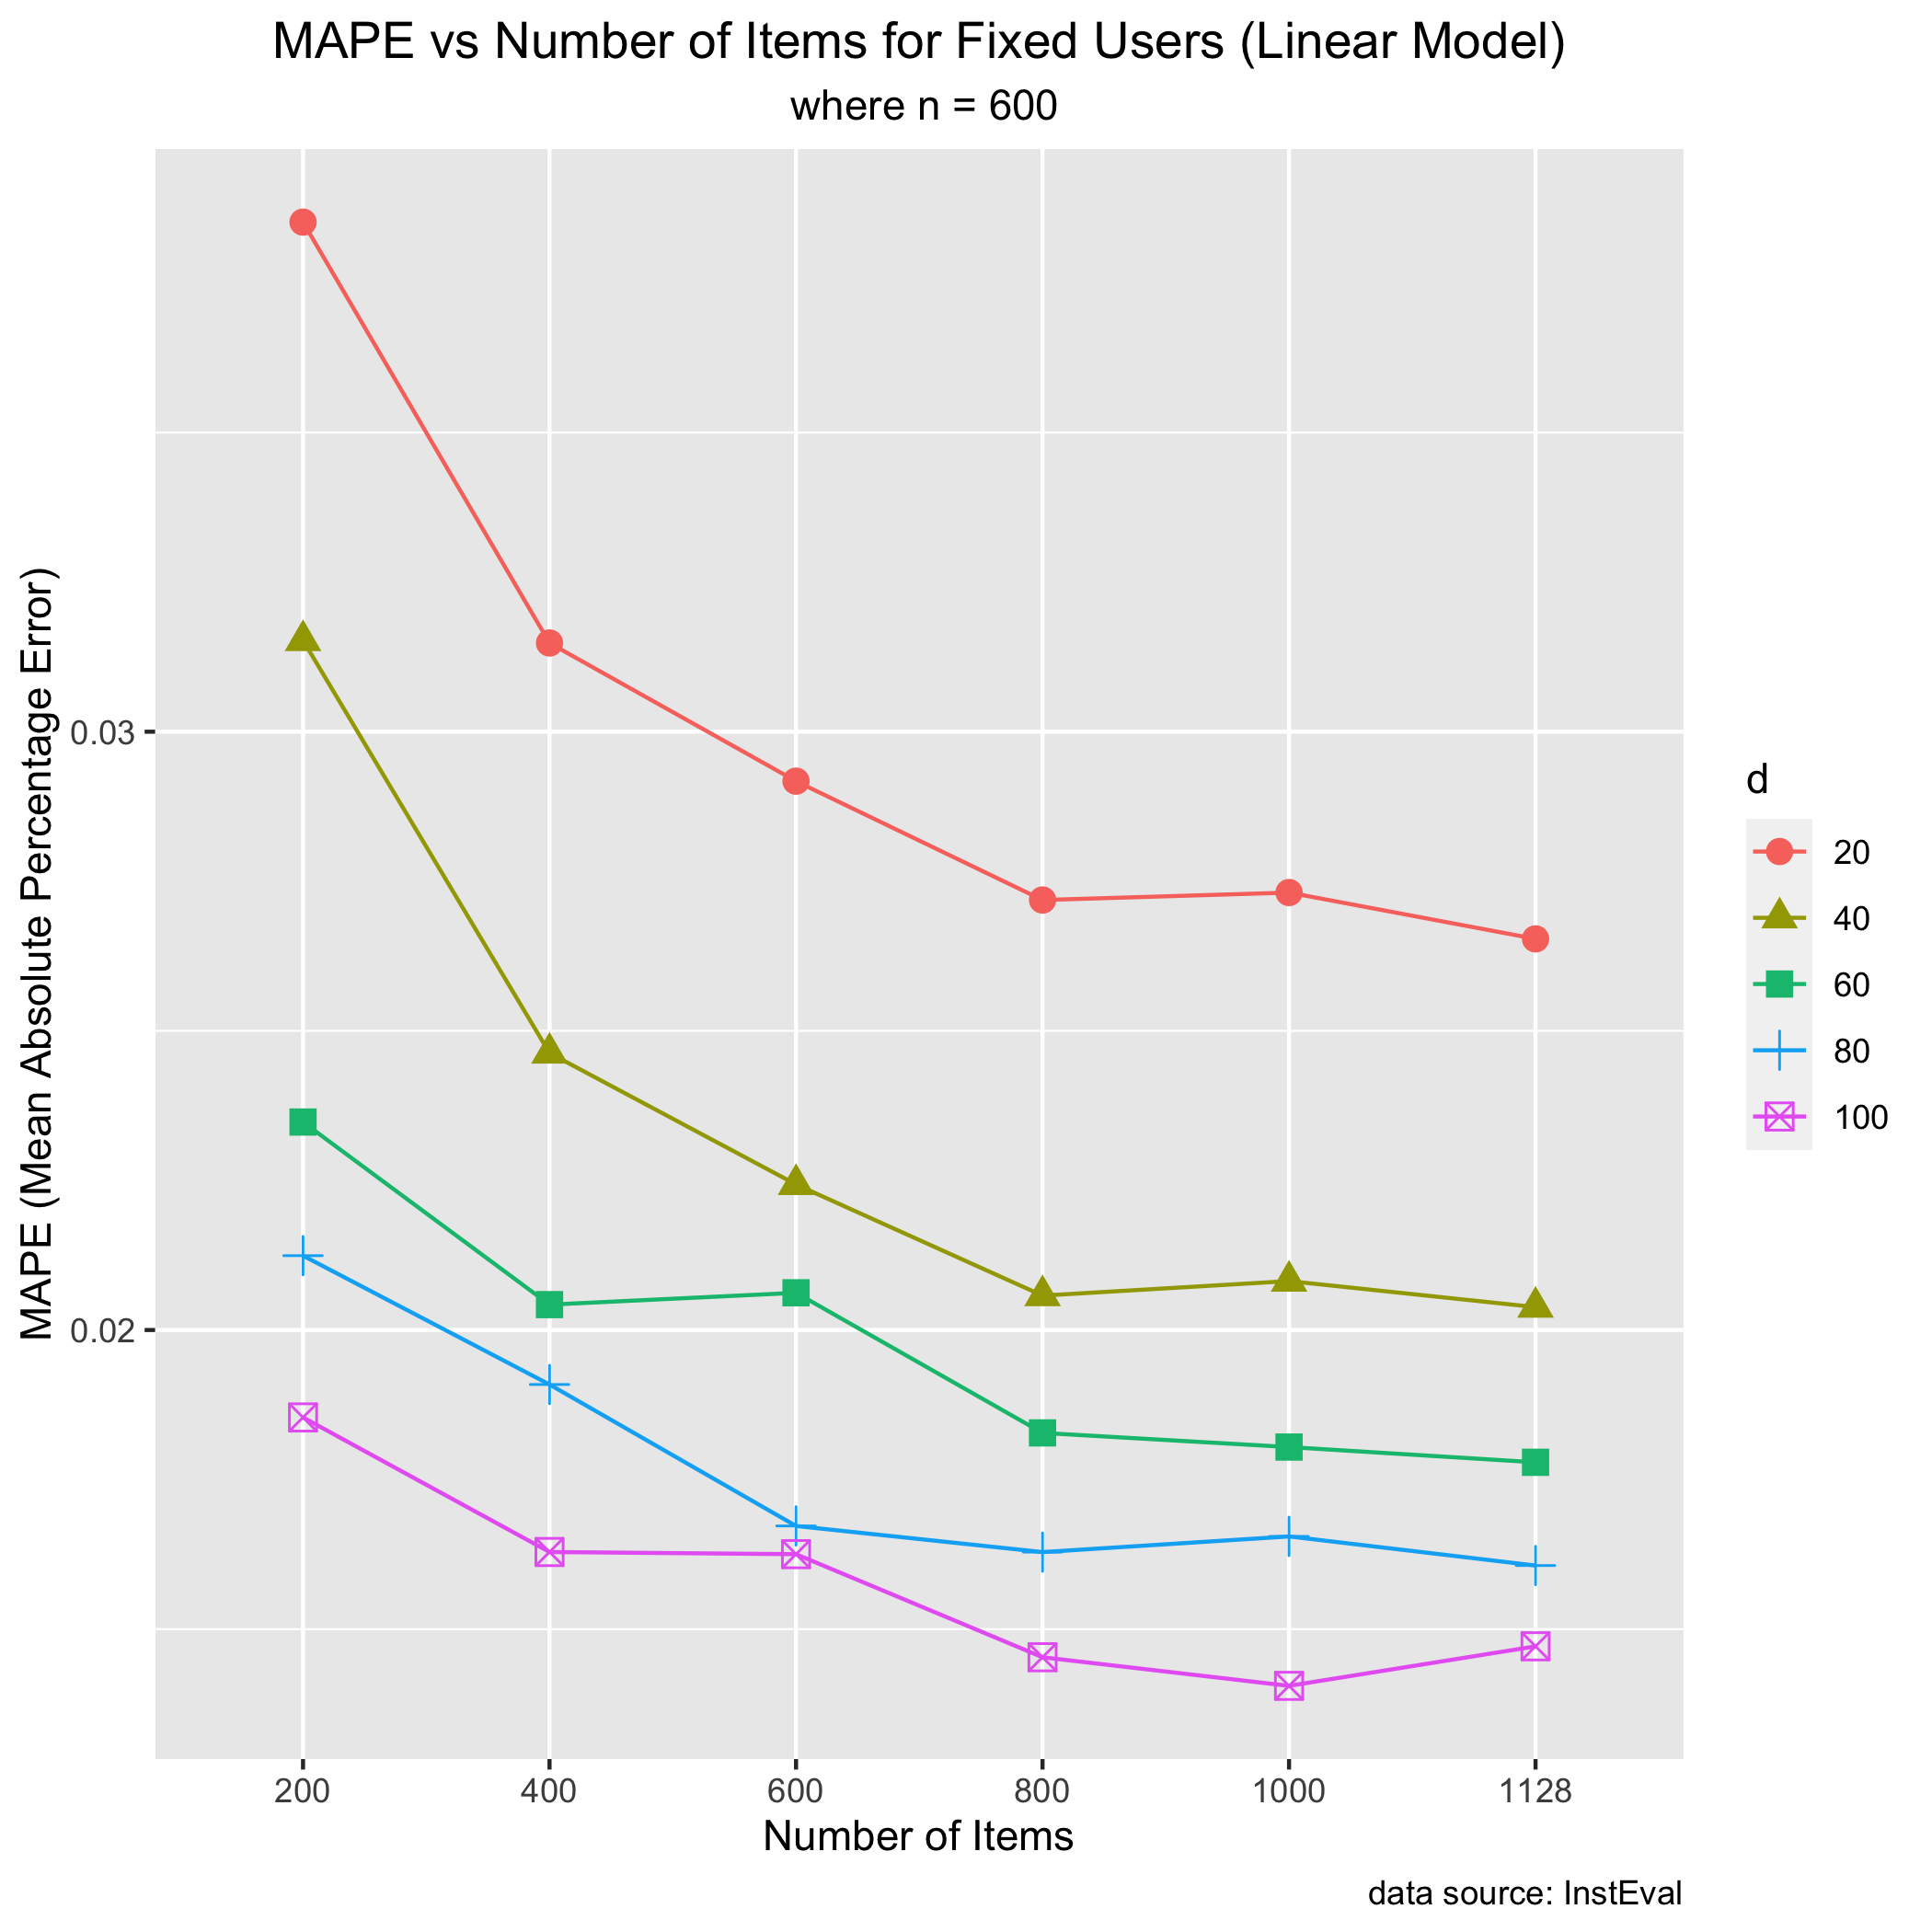
\includegraphics[width=1.2\textwidth]{MovieLens/Linear Model/n-600 (mape).png}
        \caption{n-600 (mape)}
        
    \end{minipage}\hfill
    \begin{minipage}{0.45\textwidth}
        \centering
        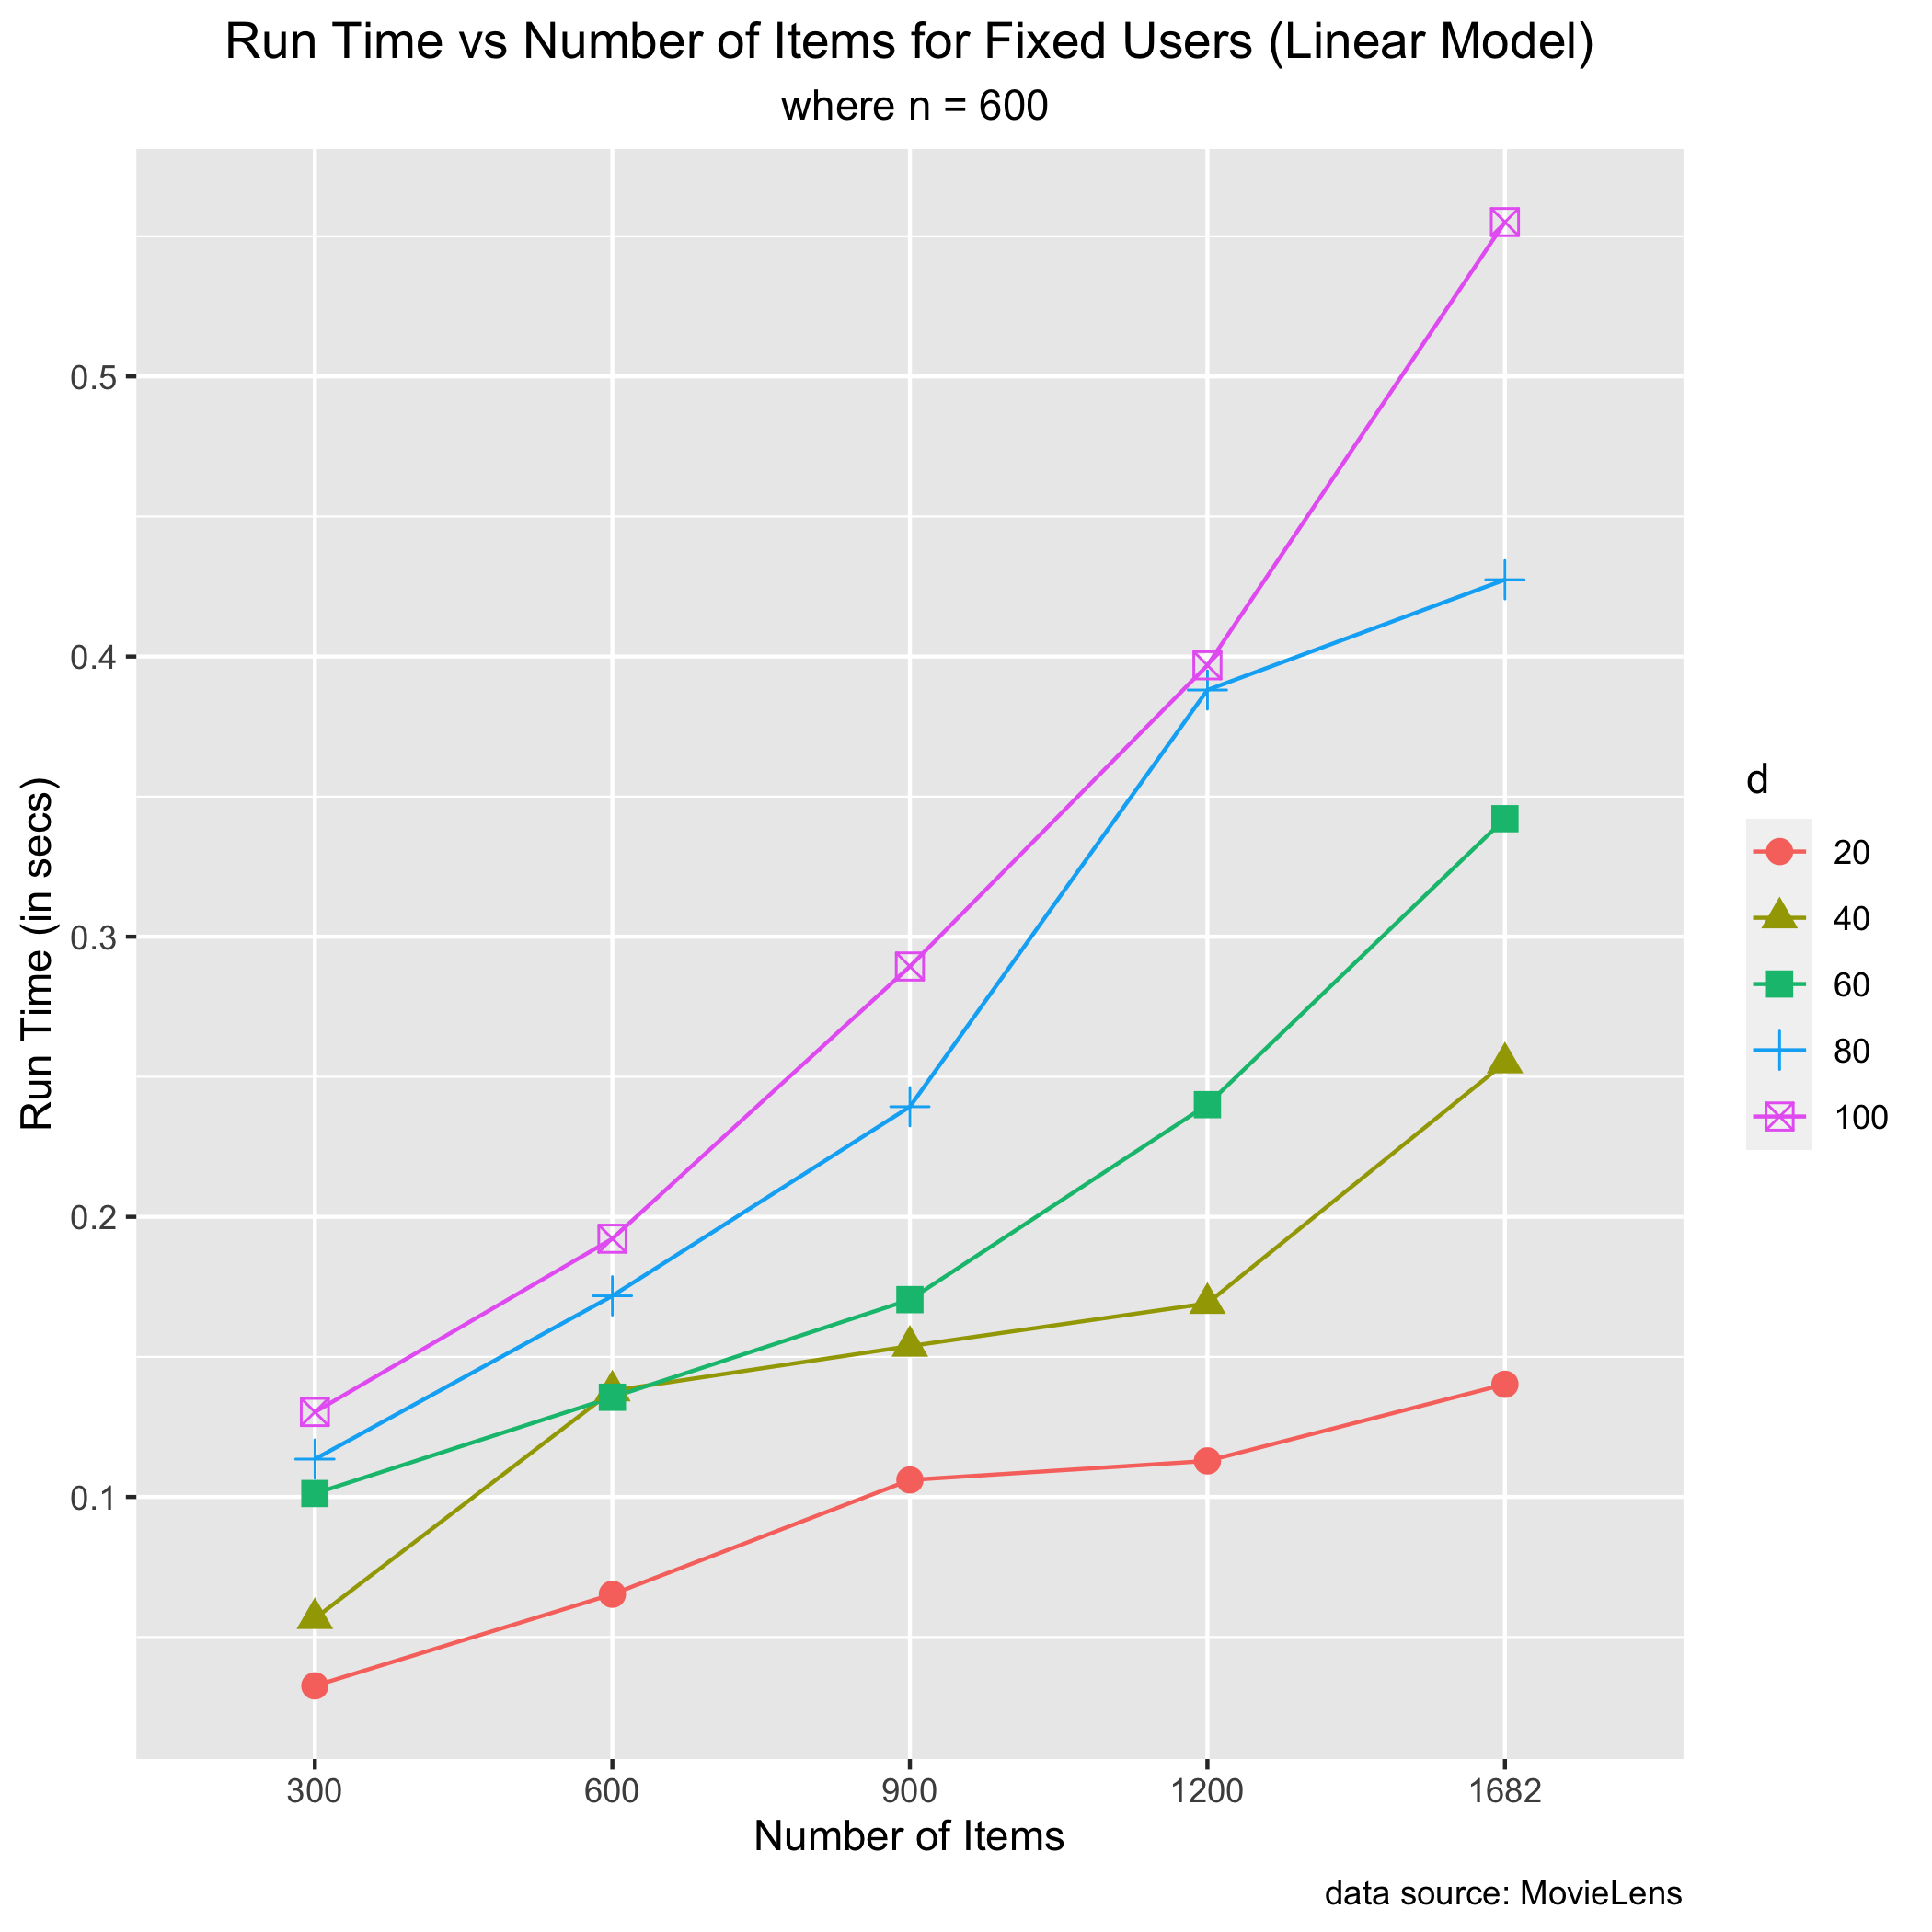
\includegraphics[width=1.2\textwidth]{MovieLens/Linear Model/n-600 (run time).png}
        \caption{n-600 (run time)}
    \end{minipage}
\end{figure}

% figure n=750
\begin{figure}[H]
\centering
    \begin{minipage}{0.45\textwidth}
        \centering
        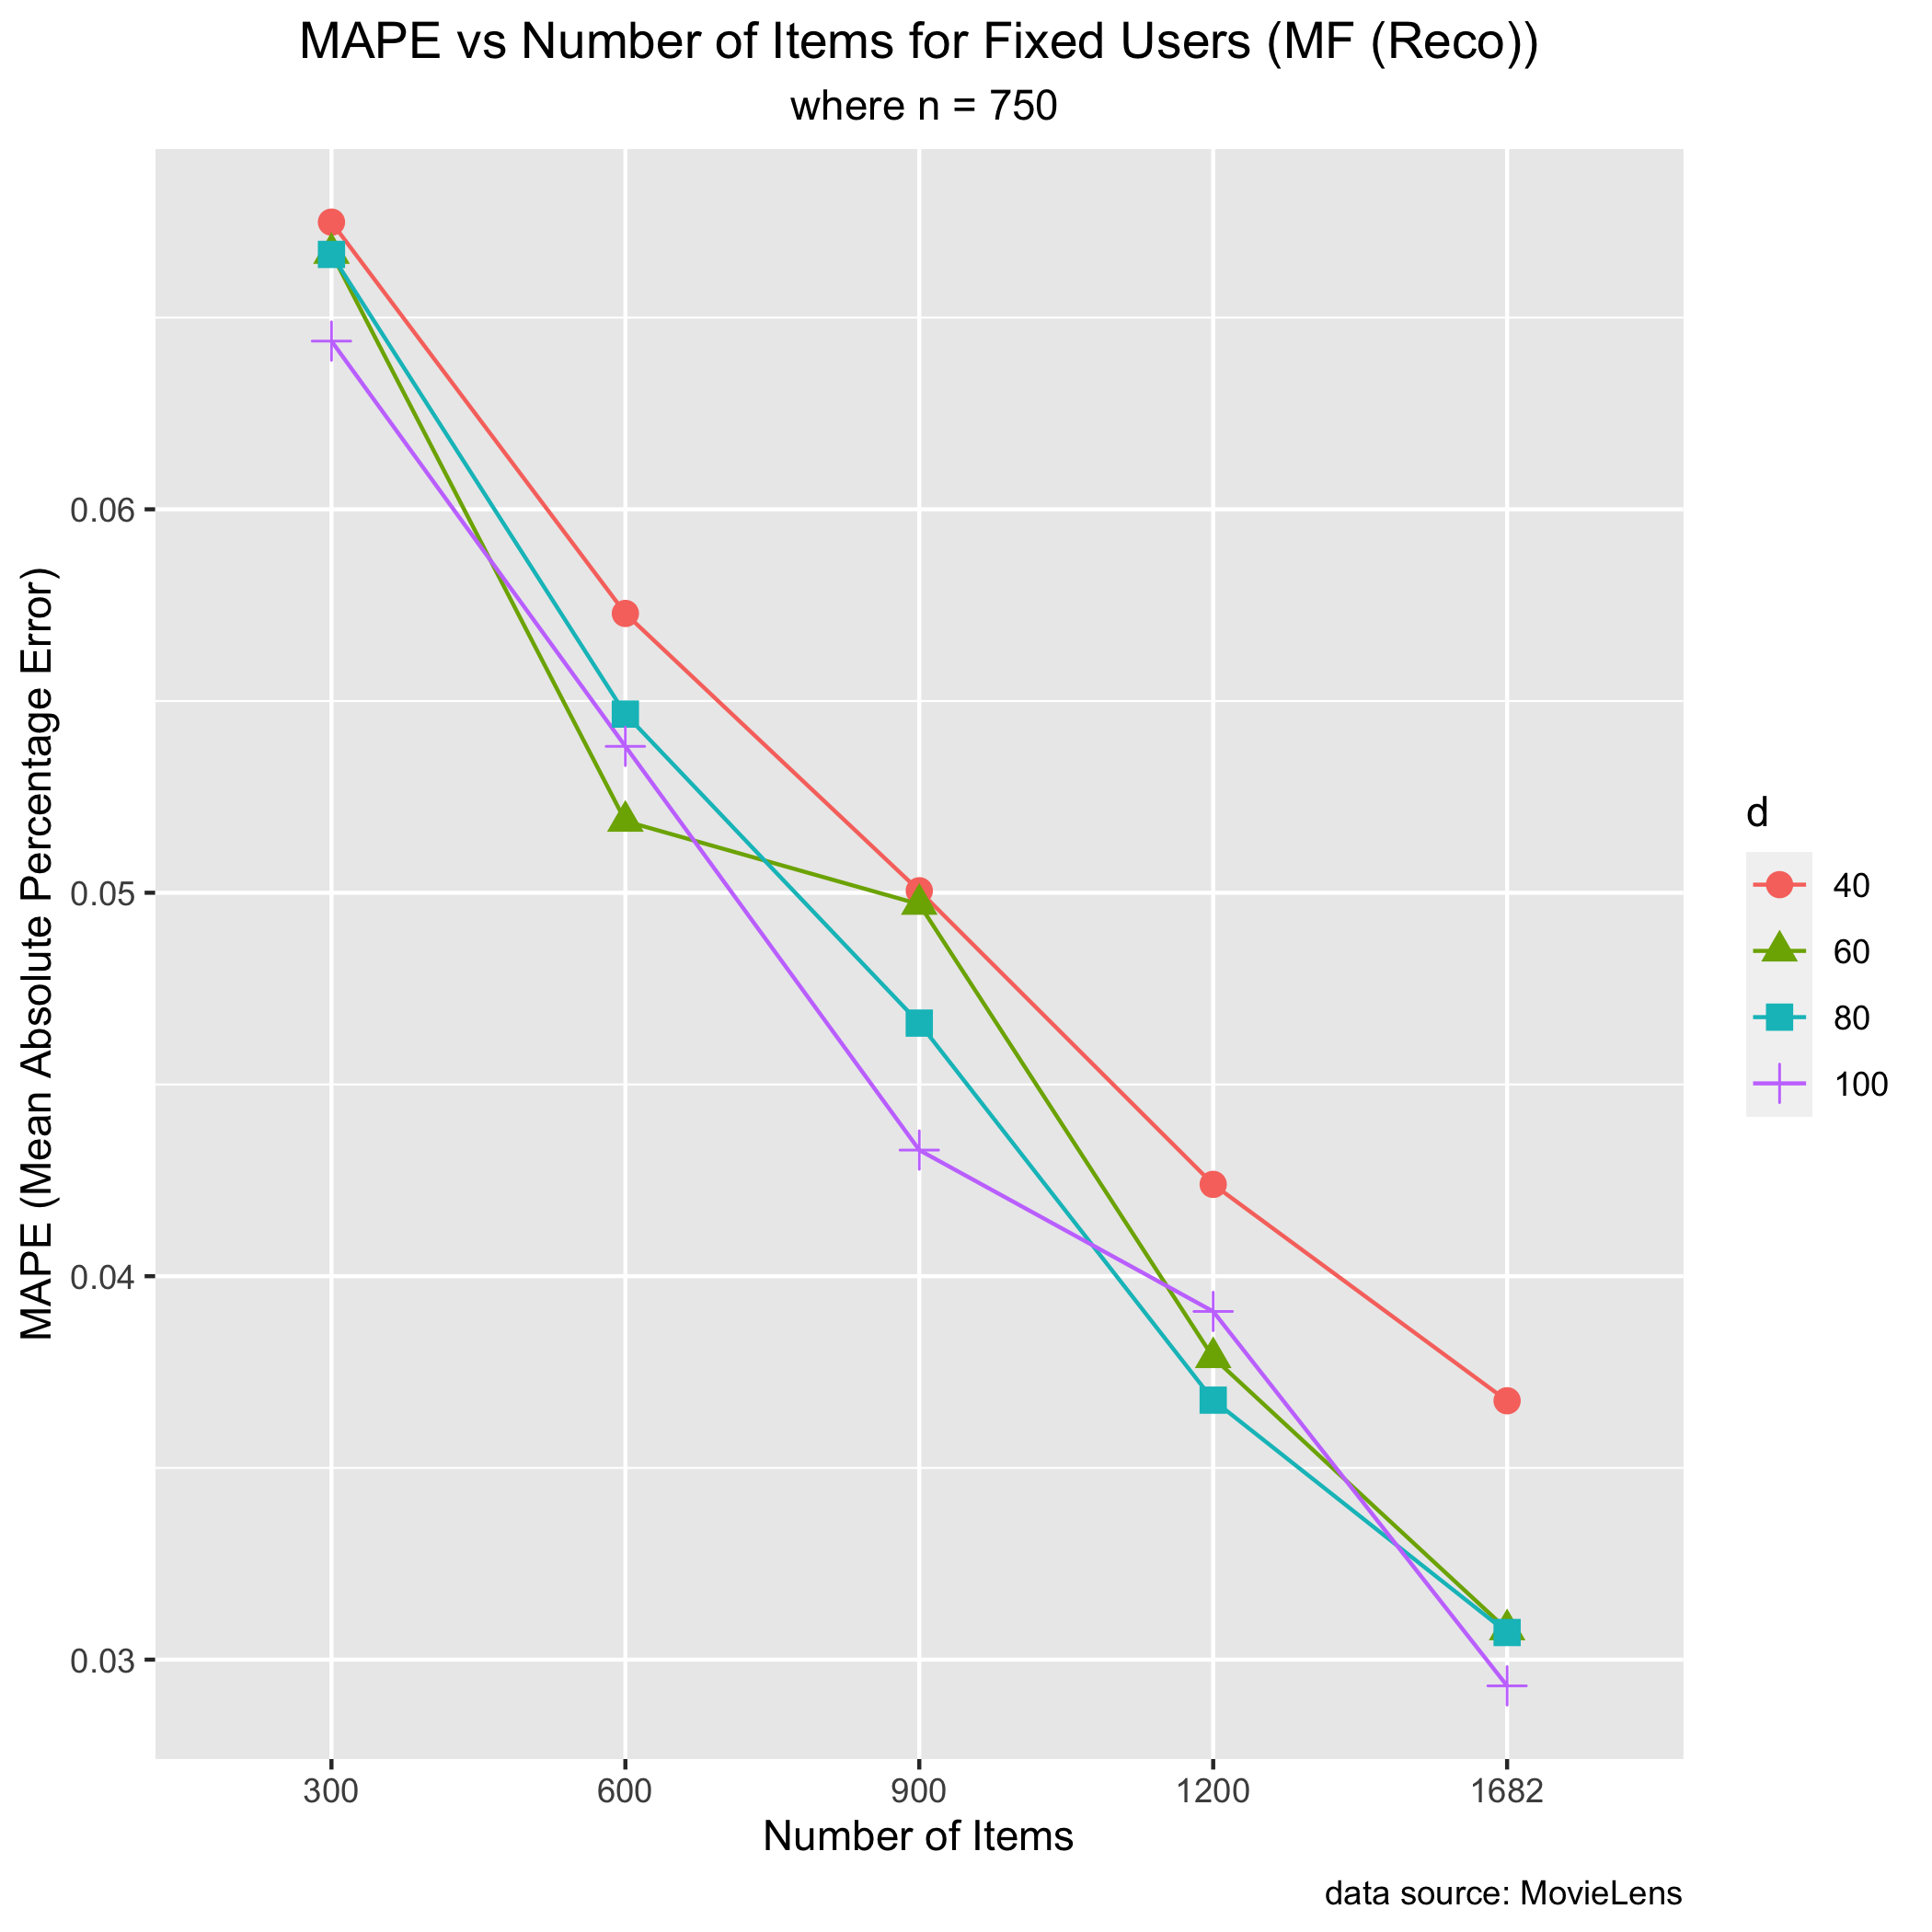
\includegraphics[width=1.2\textwidth]{MovieLens/Linear Model/n-750 (mape).png}
        \caption{n-750 (mape)}
        
    \end{minipage}\hfill
    \begin{minipage}{0.45\textwidth}
        \centering
        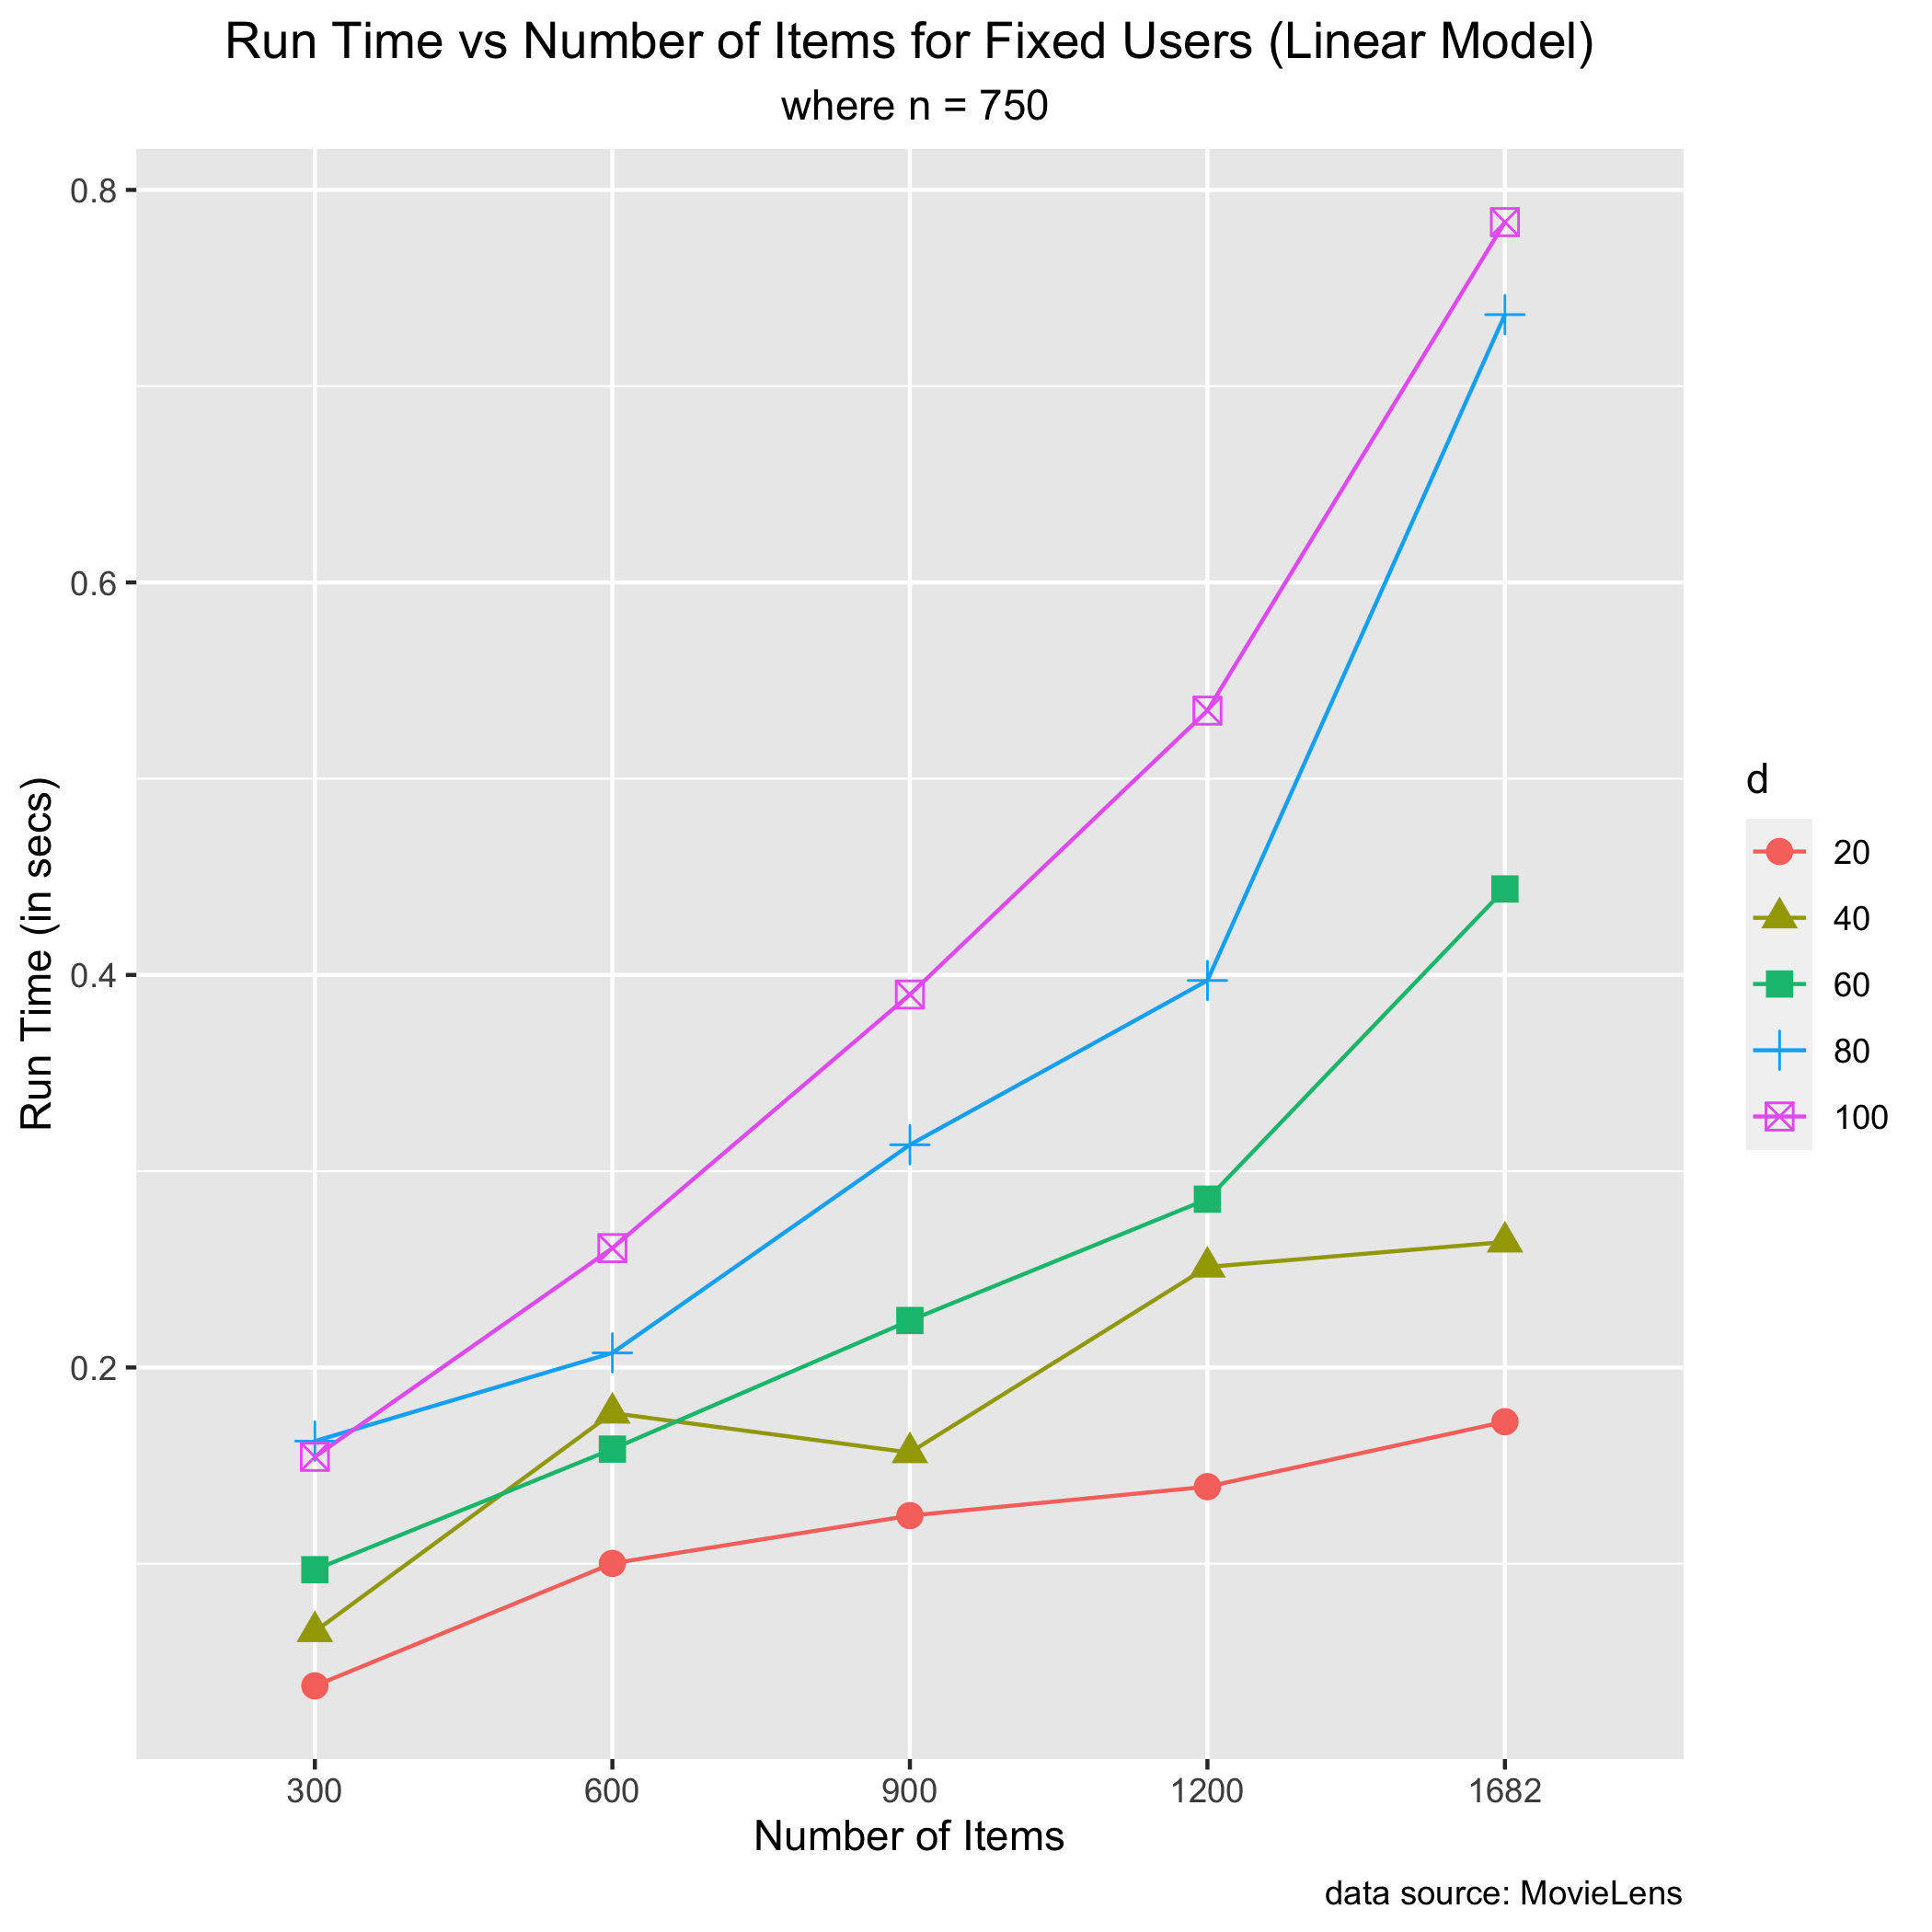
\includegraphics[width=1.2\textwidth]{MovieLens/Linear Model/n-750 (run time).png}
        \caption{n-750 (run time)}
    \end{minipage}
\end{figure}

% figure n=943
\begin{figure}[H]
\centering
    \begin{minipage}{0.45\textwidth}
        \centering
        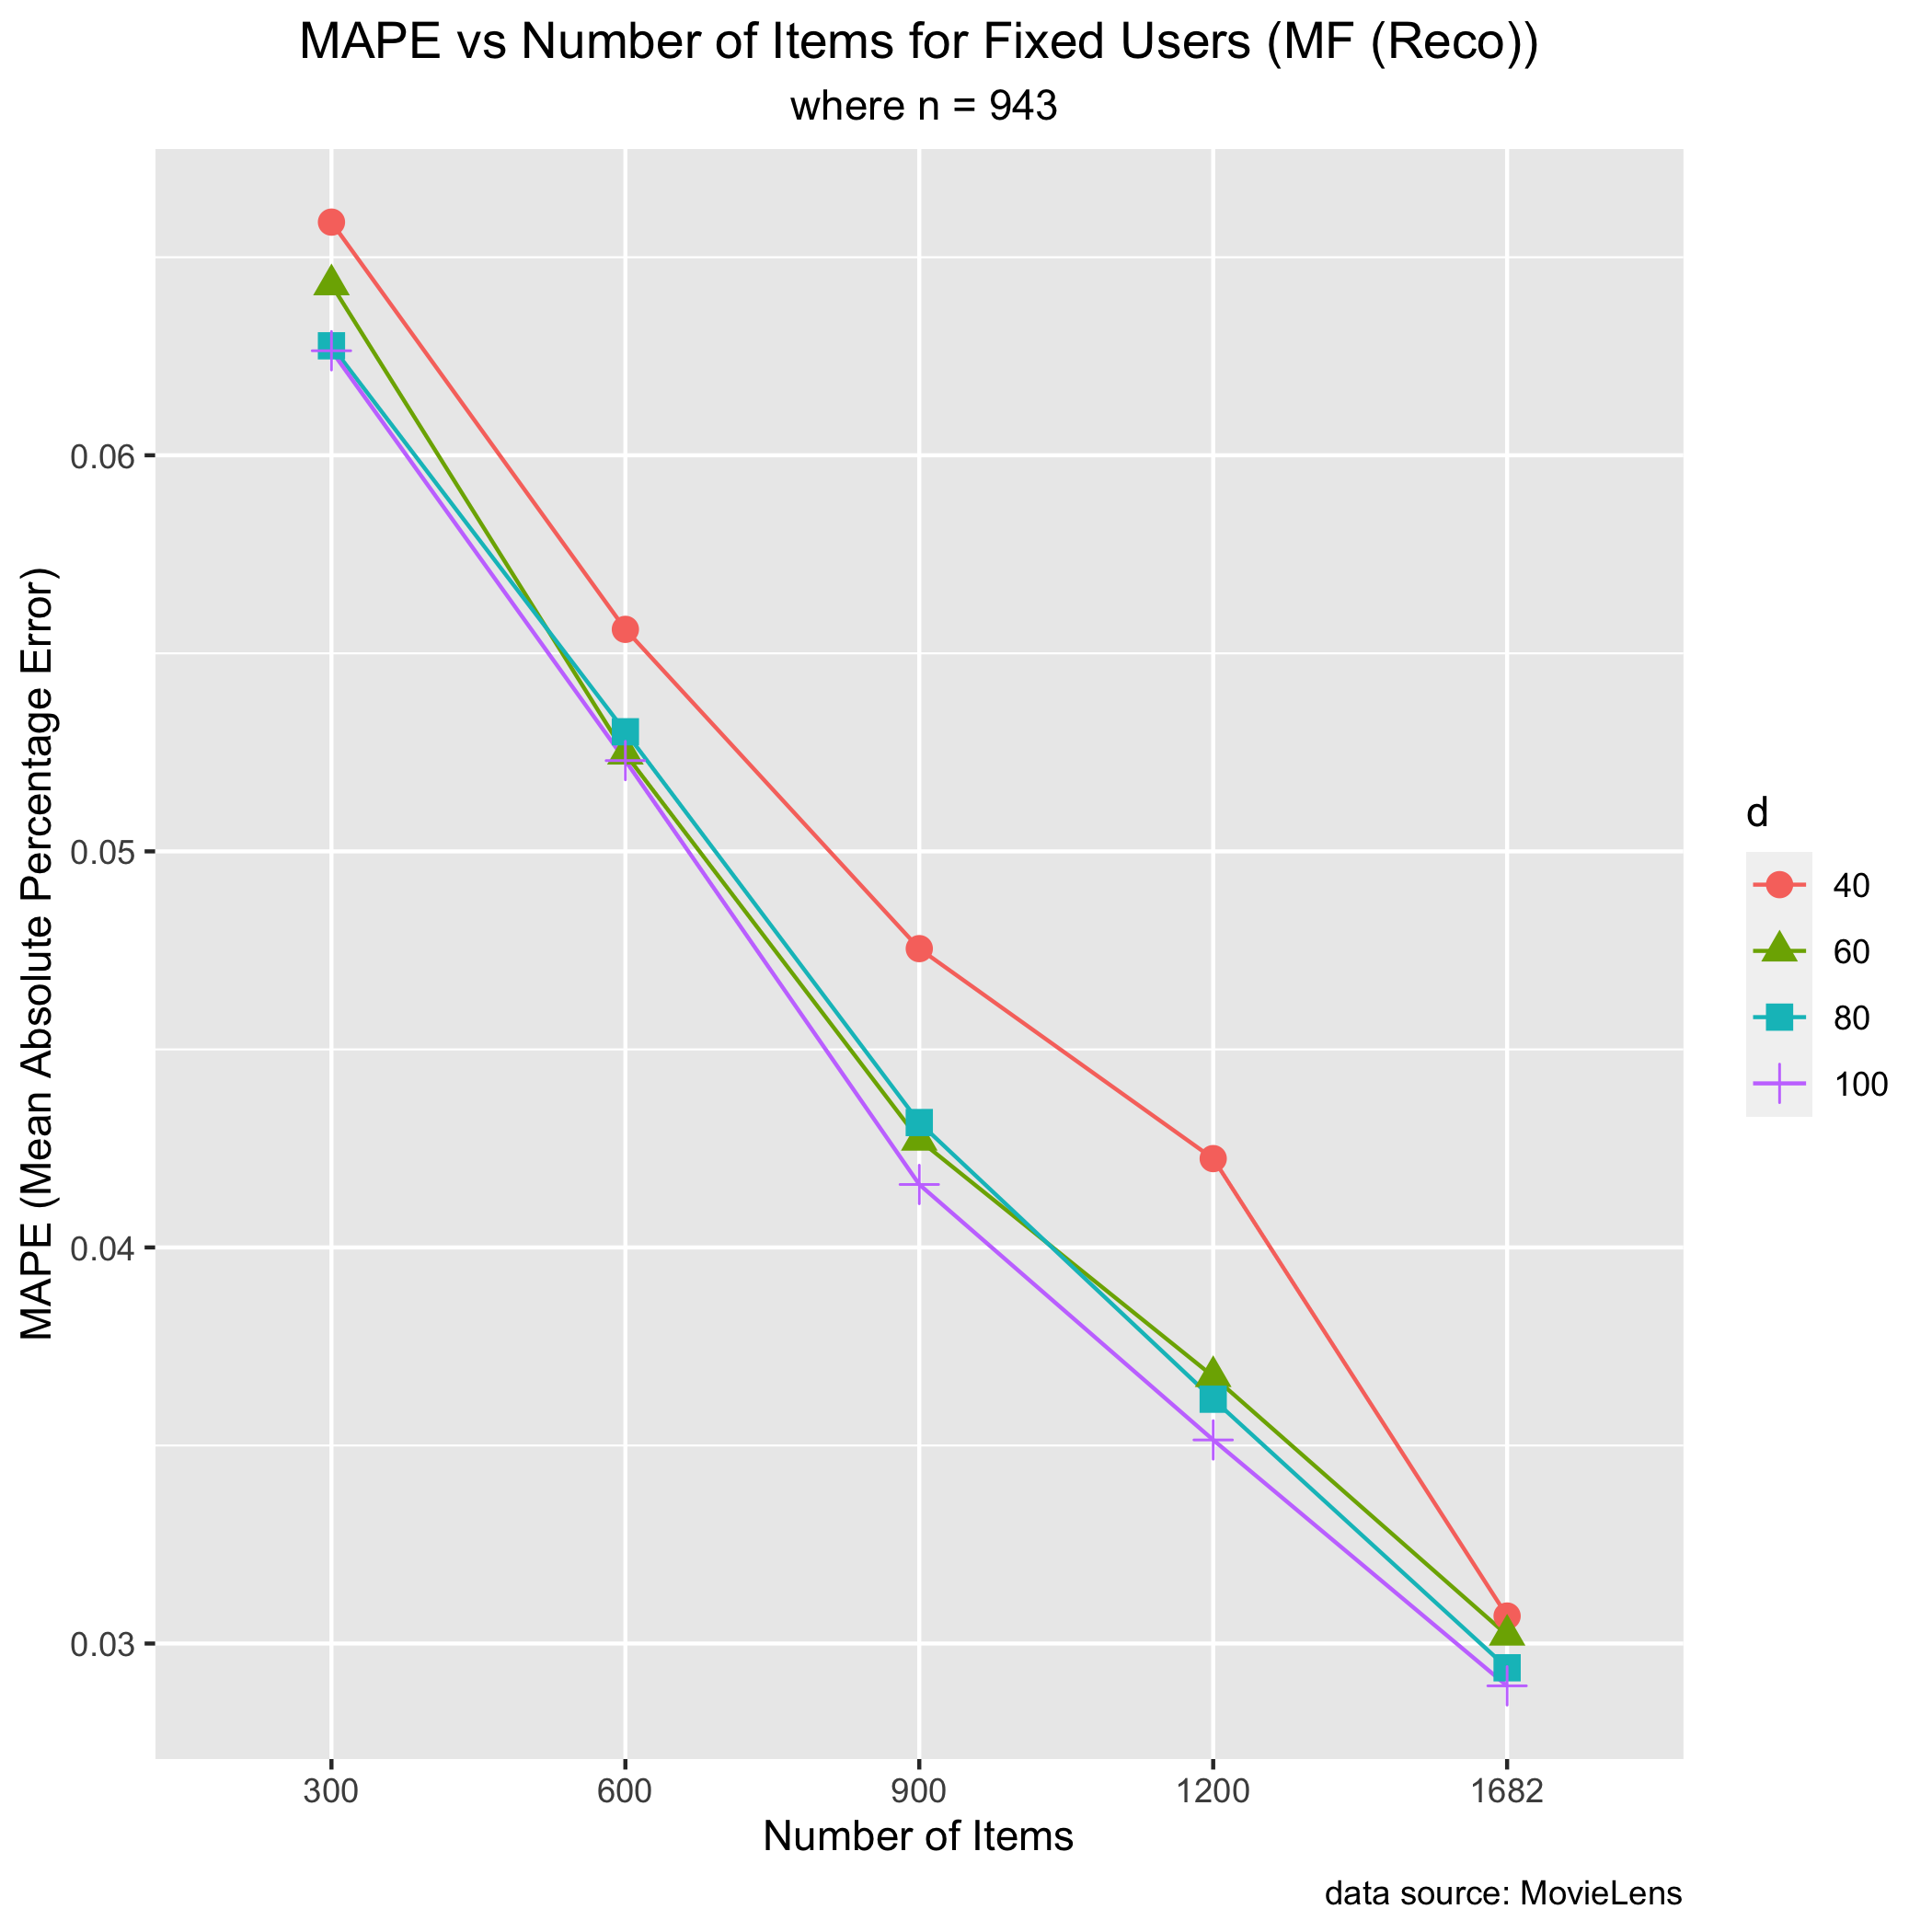
\includegraphics[width=1.2\textwidth]{MovieLens/Linear Model/n-943 (mape).png}
        \caption{n-943 (mape)}
        
    \end{minipage}\hfill
    \begin{minipage}{0.45\textwidth}
        \centering
        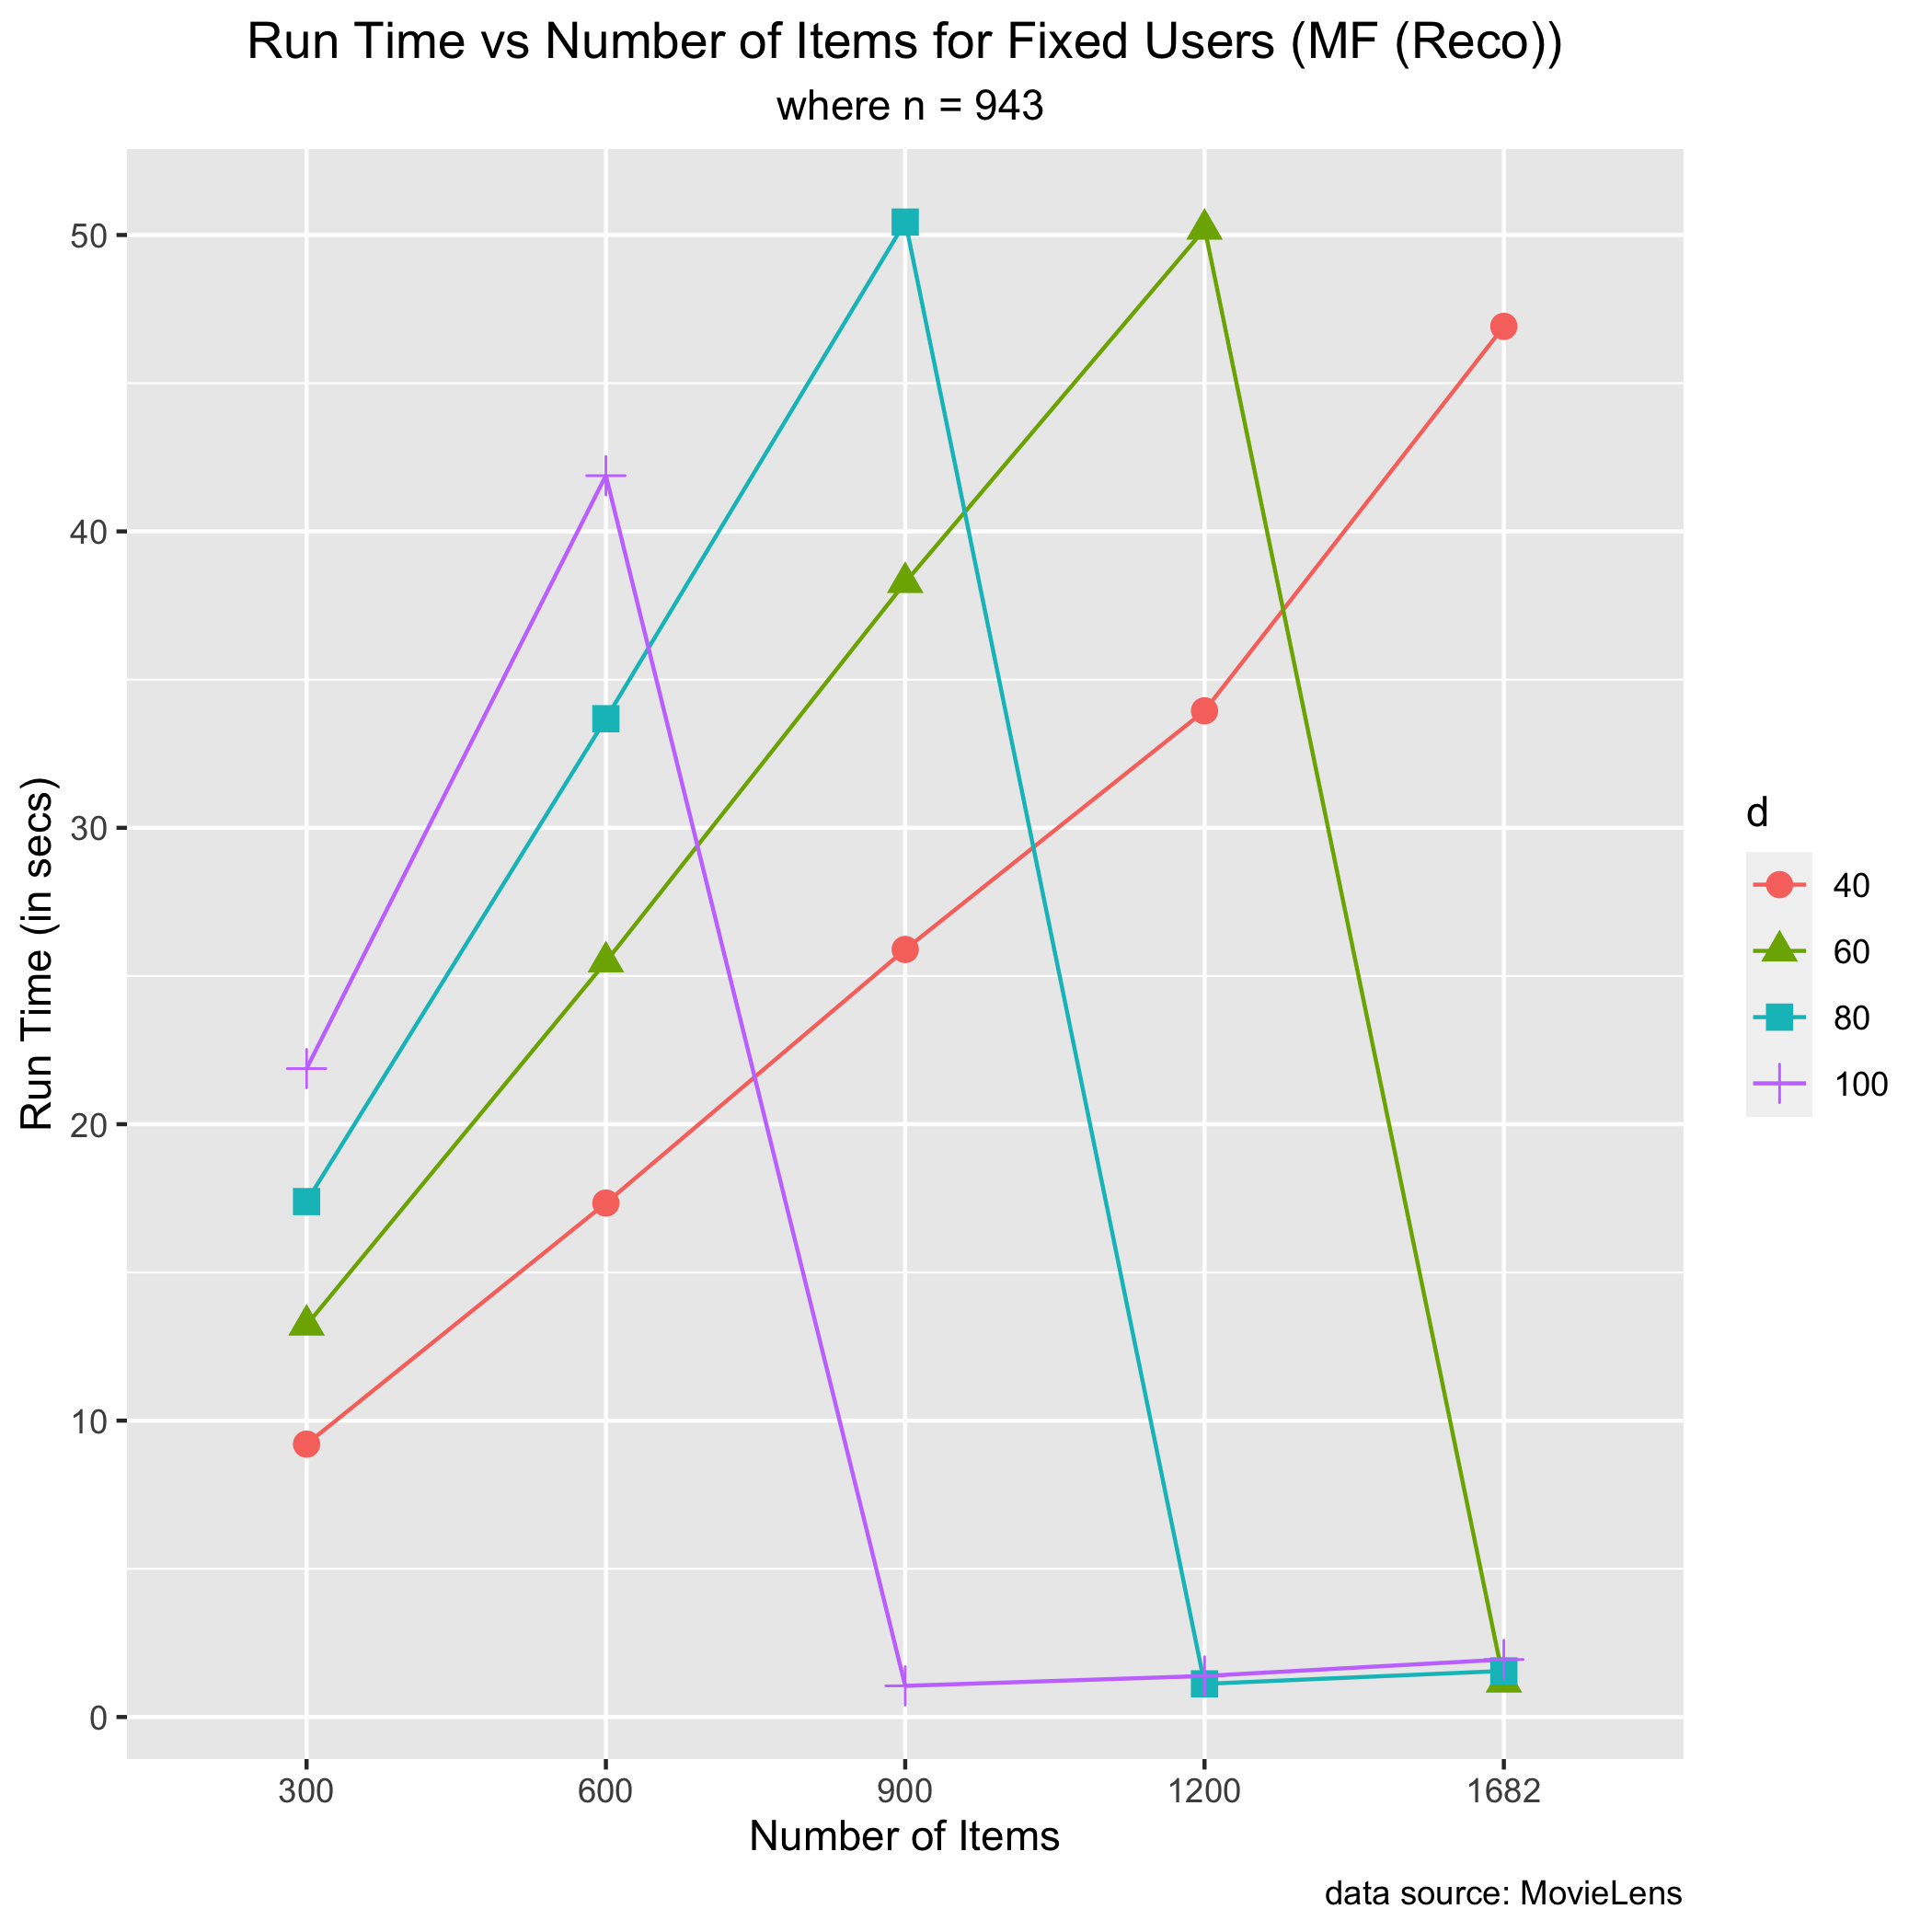
\includegraphics[width=1.2\textwidth]{MovieLens/Linear Model/n-943 (run time).png}
        \caption{n-943 (run time)}
    \end{minipage}
\end{figure}

\subsubsection{Matrix Factorization}

\paragraph{Fixed D}
\begin{itemize}
\item Compare across curves: As M increases, curves of MAPE move downward, curves of run time move upward.
\item Compare along curves: As N increases, MAPE decreases, but not significantly and run time increases. 
\end{itemize}

% figure d=20
\begin{figure}[H]
\centering
    \begin{minipage}{0.45\textwidth}
        \centering
        \includegraphics[width=1.2\textwidth]{MovieLens/MF (Reco)/d-20 (mape).png}
        \caption{d-20 (mape)}
        
    \end{minipage}\hfill
    \begin{minipage}{0.45\textwidth}
        \centering
        \includegraphics[width=1.2\textwidth]{MovieLens/MF (Reco)/d-20 (run time).png}
        \caption{d-20 (run time)}
    \end{minipage}
\end{figure}

% figure d=40
\begin{figure}[H]
\centering
    \begin{minipage}{0.45\textwidth}
        \centering
        \includegraphics[width=1.2\textwidth]{MovieLens/MF (Reco)/d-40 (mape).png}
        \caption{d-40 (mape)}
        
    \end{minipage}\hfill
    \begin{minipage}{0.45\textwidth}
        \centering
        \includegraphics[width=1.2\textwidth]{MovieLens/MF (Reco)/d-40 (run time).png}
        \caption{d-40 (run time)}
    \end{minipage}
\end{figure}

% figure d=60
\begin{figure}[H]
\centering
    \begin{minipage}{0.45\textwidth}
        \centering
        \includegraphics[width=1.2\textwidth]{MovieLens/MF (Reco)/d-60 (mape).png}
        \caption{d-60 (mape)}
        
    \end{minipage}\hfill
    \begin{minipage}{0.45\textwidth}
        \centering
        \includegraphics[width=1.2\textwidth]{MovieLens/MF (Reco)/d-60 (run time).png}
        \caption{d-60 (run time)}
    \end{minipage}
\end{figure}

% figure d=80
\begin{figure}[H]
\centering
    \begin{minipage}{0.45\textwidth}
        \centering
        \includegraphics[width=1.2\textwidth]{MovieLens/MF (Reco)/d-80 (mape).png}
        \caption{d-80 (mape)}
        
    \end{minipage}\hfill
    \begin{minipage}{0.45\textwidth}
        \centering
        \includegraphics[width=1.2\textwidth]{MovieLens/MF (Reco)/d-80 (run time).png}
        \caption{d-80 (run time)}
    \end{minipage}
\end{figure}

% figure d=100
\begin{figure}[H]
\centering
    \begin{minipage}{0.45\textwidth}
        \centering
        \includegraphics[width=1.2\textwidth]{MovieLens/MF (Reco)/d-100 (mape).png}
        \caption{d-100 (mape)}
        
    \end{minipage}\hfill
    \begin{minipage}{0.45\textwidth}
        \centering
        \includegraphics[width=1.2\textwidth]{MovieLens/MF (Reco)/d-100 (run time).png}
        \caption{d-100 (run time)}
    \end{minipage}
\end{figure}

\paragraph{Fixed M}
For all values of M, 
\begin{itemize}
\item Compare across curves:
when both M and N (number of users) are fixed, we can see a pattern where as D (ratio of non-NA values) increase, MAPE decreases in general.

\item Compare along curves:
when both M and D are fixed, the patterns between different N (number of users) values is not very distinguishable for certain N values, and details is included below. Overall, it shows a decreasing trend.
\end{itemize}

For the run time of model training, as usual, the run time increase as D or N increases.

\linebreak
\textbf{Remarks}

\begin{itemize}
    \item when M and D (propotion of non-NA values) are fixed, and N value is not large enough, such as 150, 300, 450, the increase of N doesn't significantly and necessarily decrease the MAPE. Hence, we can see even though the sample size is important for increase the accuracy, but a small increase of sample size may not effectively increase the accuracy until a large sample comes in. 
\end{itemize}

% figure m=300
\begin{figure}[H]
\centering
    \begin{minipage}{0.45\textwidth}
        \centering
        \includegraphics[width=1.2\textwidth]{MovieLens/MF (Reco)/m-300 (mape).png}
        \caption{m-300 (mape)}
        
    \end{minipage}\hfill
    \begin{minipage}{0.45\textwidth}
        \centering
        \includegraphics[width=1.2\textwidth]{MovieLens/MF (Reco)/m-300 (run time).png}
        \caption{m-300 (run time)}
    \end{minipage}
\end{figure}

% figure m=600
\begin{figure}[H]
\centering
    \begin{minipage}{0.45\textwidth}
        \centering
        \includegraphics[width=1.2\textwidth]{MovieLens/MF (Reco)/m-600 (mape).png}
        \caption{m-600 (mape)}
        
    \end{minipage}\hfill
    \begin{minipage}{0.45\textwidth}
        \centering
        \includegraphics[width=1.2\textwidth]{MovieLens/MF (Reco)/m-600 (run time).png}
        \caption{m-600 (run time)}
    \end{minipage}
\end{figure}

% figure m=900
\begin{figure}[H]
\centering
    \begin{minipage}{0.45\textwidth}
        \centering
        \includegraphics[width=1.2\textwidth]{MovieLens/MF (Reco)/m-900 (mape).png}
        \caption{m-900 (mape)}
        
    \end{minipage}\hfill
    \begin{minipage}{0.45\textwidth}
        \centering
        \includegraphics[width=1.2\textwidth]{MovieLens/MF (Reco)/m-900 (run time).png}
        \caption{m-900 (run time)}
    \end{minipage}
\end{figure}

% figure m=1200
\begin{figure}[H]
\centering
    \begin{minipage}{0.45\textwidth}
        \centering
        \includegraphics[width=1.2\textwidth]{MovieLens/MF (Reco)/m-1200 (mape).png}
        \caption{m-1200 (mape)}
        
    \end{minipage}\hfill
    \begin{minipage}{0.45\textwidth}
        \centering
        \includegraphics[width=1.2\textwidth]{MovieLens/MF (Reco)/m-1200 (run time).png}
        \caption{m-1200 (run time)}
    \end{minipage}
\end{figure}

% figure m=1682
\begin{figure}[H]
\centering
    \begin{minipage}{0.45\textwidth}
        \centering
        \includegraphics[width=1.2\textwidth]{MovieLens/MF (Reco)/m-1682 (mape).png}
        \caption{m-1682 (mape)}
        
    \end{minipage}\hfill
    \begin{minipage}{0.45\textwidth}
        \centering
        \includegraphics[width=1.2\textwidth]{MovieLens/MF (Reco)/m-1682 (run time).png}
        \caption{m-1682 (run time)}
    \end{minipage}
\end{figure}

\paragraph{Fixed N}
\begin{itemize}
\item Compare across curves: As d increases, curves of MAPE move downward, curves of run time move upward.
\item Compare along curves: As M increases, MAPE decreases and run time increases. 
\end{itemize}

% figure n=150
\begin{figure}[H]
\centering
    \begin{minipage}{0.45\textwidth}
        \centering
        \includegraphics[width=1.2\textwidth]{MovieLens/MF (Reco)/n-150 (mape).png}
        \caption{n-150 (mape)}
        
    \end{minipage}\hfill
    \begin{minipage}{0.45\textwidth}
        \centering
        \includegraphics[width=1.2\textwidth]{MovieLens/MF (Reco)/n-150 (run time).png}
        \caption{n-150 (run time)}
    \end{minipage}
\end{figure}

% figure n=300
\begin{figure}[H]
\centering
    \begin{minipage}{0.45\textwidth}
        \centering
        \includegraphics[width=1.2\textwidth]{MovieLens/MF (Reco)/n-300 (mape).png}
        \caption{n-300 (mape)}
        
    \end{minipage}\hfill
    \begin{minipage}{0.45\textwidth}
        \centering
        \includegraphics[width=1.2\textwidth]{MovieLens/MF (Reco)/n-300 (run time).png}
        \caption{n-300 (run time)}
    \end{minipage}
\end{figure}

% figure n=450
\begin{figure}[H]
\centering
    \begin{minipage}{0.45\textwidth}
        \centering
        \includegraphics[width=1.2\textwidth]{MovieLens/MF (Reco)/n-450 (mape).png}
        \caption{n-450 (mape)}
        
    \end{minipage}\hfill
    \begin{minipage}{0.45\textwidth}
        \centering
        \includegraphics[width=1.2\textwidth]{MovieLens/MF (Reco)/n-450 (run time).png}
        \caption{n-450 (run time)}
    \end{minipage}
\end{figure}

% figure n=600
\begin{figure}[H]
\centering
    \begin{minipage}{0.45\textwidth}
        \centering
        \includegraphics[width=1.2\textwidth]{MovieLens/MF (Reco)/n-600 (mape).png}
        \caption{n-600 (mape)}
        
    \end{minipage}\hfill
    \begin{minipage}{0.45\textwidth}
        \centering
        \includegraphics[width=1.2\textwidth]{MovieLens/MF (Reco)/n-600 (run time).png}
        \caption{n-600 (run time)}
    \end{minipage}
\end{figure}

% figure n=750
\begin{figure}[H]
\centering
    \begin{minipage}{0.45\textwidth}
        \centering
        \includegraphics[width=1.2\textwidth]{MovieLens/MF (Reco)/n-750 (mape).png}
        \caption{n-750 (mape)}
        
    \end{minipage}\hfill
    \begin{minipage}{0.45\textwidth}
        \centering
        \includegraphics[width=1.2\textwidth]{MovieLens/MF (Reco)/n-750 (run time).png}
        \caption{n-750 (run time)}
    \end{minipage}
\end{figure}

% figure n=943
\begin{figure}[H]
\centering
    \begin{minipage}{0.45\textwidth}
        \centering
        \includegraphics[width=1.2\textwidth]{MovieLens/MF (Reco)/n-943 (mape).png}
        \caption{n-943 (mape)}
        
    \end{minipage}\hfill
    \begin{minipage}{0.45\textwidth}
        \centering
        \includegraphics[width=1.2\textwidth]{MovieLens/MF (Reco)/n-943 (run time).png}
        \caption{n-943 (run time)}
    \end{minipage}
\end{figure}


% \iffalse %comment out InstEval for faster compilation
\subsection{InstEval}
\subsubsection{Linear Model}

\paragraph{Fixed D}
\begin{itemize}
\item Compare across curves: As m increases, curves of MAPE move downward, curves of run time move upward.
\item Compare along curves: As N increases, MAPE decreases and run time increases. 
\end{itemize}

% figure d=20
\begin{figure}[H]
\centering
    \begin{minipage}{0.45\textwidth}
        \centering
        \includegraphics[width=1.2\textwidth]{InstEval/Linear Model/d-20 (mape).png}
        \caption{d-20 (mape)}
        
    \end{minipage}\hfill
    \begin{minipage}{0.45\textwidth}
        \centering
        \includegraphics[width=1.2\textwidth]{InstEval/Linear Model/d-20 (run time).png}
        \caption{d-20 (run time)}
    \end{minipage}
\end{figure}

% figure d=40
\begin{figure}[H]
\centering
    \begin{minipage}{0.45\textwidth}
        \centering
        \includegraphics[width=1.2\textwidth]{InstEval/Linear Model/d-40 (mape).png}
        \caption{d-40 (mape)}
        
    \end{minipage}\hfill
    \begin{minipage}{0.45\textwidth}
        \centering
        \includegraphics[width=1.2\textwidth]{InstEval/Linear Model/d-40 (run time).png}
        \caption{d-40 (run time)}
    \end{minipage}
\end{figure}

% figure d=60
\begin{figure}[H]
\centering
    \begin{minipage}{0.45\textwidth}
        \centering
        \includegraphics[width=1.2\textwidth]{InstEval/Linear Model/d-60 (mape).png}
        \caption{d-60 (mape)}
        
    \end{minipage}\hfill
    \begin{minipage}{0.45\textwidth}
        \centering
        \includegraphics[width=1.2\textwidth]{InstEval/Linear Model/d-60 (run time).png}
        \caption{d-60 (run time)}
    \end{minipage}
\end{figure}

% figure d=80
\begin{figure}[H]
\centering
    \begin{minipage}{0.45\textwidth}
        \centering
        \includegraphics[width=1.2\textwidth]{InstEval/Linear Model/d-80 (mape).png}
        \caption{d-80 (mape)}
        
    \end{minipage}\hfill
    \begin{minipage}{0.45\textwidth}
        \centering
        \includegraphics[width=1.2\textwidth]{InstEval/Linear Model/d-80 (run time).png}
        \caption{d-80 (run time)}
    \end{minipage}
\end{figure}

% figure d=100
\begin{figure}[H]
\centering
    \begin{minipage}{0.45\textwidth}
        \centering
        \includegraphics[width=1.2\textwidth]{InstEval/Linear Model/d-100 (mape).png}
        \caption{d-100 (mape)}
        
    \end{minipage}\hfill
    \begin{minipage}{0.45\textwidth}
        \centering
        \includegraphics[width=1.2\textwidth]{InstEval/Linear Model/d-100 (run time).png}
        \caption{d-100 (run time)}
    \end{minipage}
\end{figure}

\paragraph{Fixed M}
\begin{itemize}
\item Compare across curves: As n increases, curves of MAPE move downward, curves of run time move upward.
\item Compare along curves: As d increases, MAPE decreases and run time increases. 
\end{itemize}


% figure m=200
\begin{figure}[H]
\centering
    \begin{minipage}{0.45\textwidth}
        \centering
        \includegraphics[width=1.2\textwidth]{InstEval/Linear Model/m-200 (mape).png}
        \caption{m-200 (mape)}
        
    \end{minipage}\hfill
    \begin{minipage}{0.45\textwidth}
        \centering
        \includegraphics[width=1.2\textwidth]{InstEval/Linear Model/m-200 (run time).png}
        \caption{m-200 (run time)}
    \end{minipage}
\end{figure}

% figure m=400
\begin{figure}[H]
\centering
    \begin{minipage}{0.45\textwidth}
        \centering
        \includegraphics[width=1.2\textwidth]{InstEval/Linear Model/m-400 (mape).png}
        \caption{m-400 (mape)}
        
    \end{minipage}\hfill
    \begin{minipage}{0.45\textwidth}
        \centering
        \includegraphics[width=1.2\textwidth]{InstEval/Linear Model/m-400 (run time).png}
        \caption{m-400 (run time)}
    \end{minipage}
\end{figure}

% figure m=600
\begin{figure}[H]
\centering
    \begin{minipage}{0.45\textwidth}
        \centering
        \includegraphics[width=1.2\textwidth]{InstEval/Linear Model/m-600 (mape).png}
        \caption{m-600 (mape)}
        
    \end{minipage}\hfill
    \begin{minipage}{0.45\textwidth}
        \centering
        \includegraphics[width=1.2\textwidth]{InstEval/Linear Model/m-600 (run time).png}
        \caption{m-600 (run time)}
    \end{minipage}
\end{figure}

% figure m=800
\begin{figure}[H]
\centering
    \begin{minipage}{0.45\textwidth}
        \centering
        \includegraphics[width=1.2\textwidth]{InstEval/Linear Model/m-800 (mape).png}
        \caption{m-800 (mape)}
        
    \end{minipage}\hfill
    \begin{minipage}{0.45\textwidth}
        \centering
        \includegraphics[width=1.2\textwidth]{InstEval/Linear Model/m-800 (run time).png}
        \caption{m-800 (run time)}
    \end{minipage}
\end{figure}

% figure m=1000
\begin{figure}[H]
\centering
    \begin{minipage}{0.45\textwidth}
        \centering
        \includegraphics[width=1.2\textwidth]{InstEval/Linear Model/m-1000 (mape).png}
        \caption{m-1000 (mape)}
        
    \end{minipage}\hfill
    \begin{minipage}{0.45\textwidth}
        \centering
        \includegraphics[width=1.2\textwidth]{InstEval/Linear Model/m-1000 (run time).png}
        \caption{m-1000 (run time)}
    \end{minipage}
\end{figure}

% figure m=1128
\begin{figure}[H]
\centering
    \begin{minipage}{0.45\textwidth}
        \centering
        \includegraphics[width=1.2\textwidth]{InstEval/Linear Model/m-1128 (mape).png}
        \caption{m-1128 (mape)}
        
    \end{minipage}\hfill
    \begin{minipage}{0.45\textwidth}
        \centering
        \includegraphics[width=1.2\textwidth]{InstEval/Linear Model/m-1128 (run time).png}
        \caption{m-1128 (run time)}
    \end{minipage}
\end{figure}

\paragraph{Fixed N}
\begin{itemize}
\item Compare across curves: As m increases, curves of MAPE move downward, curves of run time move upward.
\item Compare along curves: As N increases, MAPE decreases slightly at the end, but the trend is not as strong as the previous ones. As N increases, run time increases. 
\end{itemize}

% figure n=200
\begin{figure}[H]
\centering
    \begin{minipage}{0.45\textwidth}
        \centering
        \includegraphics[width=1.2\textwidth]{InstEval/Linear Model/n-200 (mape).png}
        \caption{n-200 (mape)}
        \label{fig:figure1}
    \end{minipage}\hfill
    \begin{minipage}{0.45\textwidth}
        \centering
        \includegraphics[width=1.2\textwidth]{InstEval/Linear Model/n-200 (run time).png}
        \caption{n-200 (run time)}
    \end{minipage}
\end{figure}

% figure n=400
\begin{figure}[H]
\centering
    \begin{minipage}{0.45\textwidth}
        \centering
        \includegraphics[width=1.2\textwidth]{InstEval/Linear Model/n-400 (mape).png}
        \caption{n-400 (mape)}
        \label{fig:figure1}
    \end{minipage}\hfill
    \begin{minipage}{0.45\textwidth}
        \centering
        \includegraphics[width=1.2\textwidth]{InstEval/Linear Model/n-400 (run time).png}
        \caption{n-400 (run time)}
    \end{minipage}
\end{figure}

% figure n=600
\begin{figure}[H]
\centering
    \begin{minipage}{0.45\textwidth}
        \centering
        \includegraphics[width=1.2\textwidth]{InstEval/Linear Model/n-600 (mape).png}
        \caption{n-600 (mape)}
        \label{fig:figure1}
    \end{minipage}\hfill
    \begin{minipage}{0.45\textwidth}
        \centering
        \includegraphics[width=1.2\textwidth]{InstEval/Linear Model/n-600 (run time).png}
        \caption{n-600 (run time)}
    \end{minipage}
\end{figure}

% figure n=800
\begin{figure}[H]
\centering
    \begin{minipage}{0.45\textwidth}
        \centering
        \includegraphics[width=1.2\textwidth]{InstEval/Linear Model/n-800 (mape).png}
        \caption{n-800 (mape)}
        \label{fig:figure1}
    \end{minipage}\hfill
    \begin{minipage}{0.45\textwidth}
        \centering
        \includegraphics[width=1.2\textwidth]{InstEval/Linear Model/n-800 (run time).png}
        \caption{n-800 (run time)}
    \end{minipage}
\end{figure}

% figure n=1000
\begin{figure}[H]
\centering
    \begin{minipage}{0.45\textwidth}
        \centering
        \includegraphics[width=1.2\textwidth]{InstEval/Linear Model/n-1000 (mape).png}
        \caption{n-1000 (mape)}
        \label{fig:figure1}
    \end{minipage}\hfill
    \begin{minipage}{0.45\textwidth}
        \centering
        \includegraphics[width=1.2\textwidth]{InstEval/Linear Model/n-1000 (run time).png}
        \caption{n-1000 (run time)}
    \end{minipage}
\end{figure}

% figure n=1216
\begin{figure}[H]
\centering
    \begin{minipage}{0.45\textwidth}
        \centering
        \includegraphics[width=1.2\textwidth]{InstEval/Linear Model/n-1216 (mape).png}
        \caption{n-1216 (mape)}
        \label{fig:figure1}
    \end{minipage}\hfill
    \begin{minipage}{0.45\textwidth}
        \centering
        \includegraphics[width=1.2\textwidth]{InstEval/Linear Model/n-1216 (run time).png}
        \caption{n-1216 (run time)}
    \end{minipage}
\end{figure}



\subsubsection{Matrix Factorization}

\paragraph{Fixed D}
\begin{itemize}
\item Compare across curves: As m increases, curves of MAPE move downward, curves of run time move upward.
\item Compare along curves: As N increases, MAPE decreases and run time increases. 
\end{itemize}

% figure d=20
\begin{figure}[H]
\centering
    \begin{minipage}{0.45\textwidth}
        \centering
        \includegraphics[width=1.2\textwidth]{InstEval/MF (Reco)/d-20 (mape).png}
        \caption{d-20 (mape)}
        
    \end{minipage}\hfill
    \begin{minipage}{0.45\textwidth}
        \centering
        \includegraphics[width=1.2\textwidth]{InstEval/MF (Reco)/d-20 (run time).png}
        \caption{d-20 (run time)}
    \end{minipage}
\end{figure}

% figure d=40
\begin{figure}[H]
\centering
    \begin{minipage}{0.45\textwidth}
        \centering
        \includegraphics[width=1.2\textwidth]{InstEval/MF (Reco)/d-40 (mape).png}
        \caption{d-40 (mape)}
        
    \end{minipage}\hfill
    \begin{minipage}{0.45\textwidth}
        \centering
        \includegraphics[width=1.2\textwidth]{InstEval/MF (Reco)/d-40 (run time).png}
        \caption{d-40 (run time)}
    \end{minipage}
\end{figure}

% figure d=60
\begin{figure}[H]
\centering
    \begin{minipage}{0.45\textwidth}
        \centering
        \includegraphics[width=1.2\textwidth]{InstEval/MF (Reco)/d-60 (mape).png}
        \caption{d-60 (mape)}
        
    \end{minipage}\hfill
    \begin{minipage}{0.45\textwidth}
        \centering
        \includegraphics[width=1.2\textwidth]{InstEval/MF (Reco)/d-60 (run time).png}
        \caption{d-60 (run time)}
    \end{minipage}
\end{figure}

% figure d=80
\begin{figure}[H]
\centering
    \begin{minipage}{0.45\textwidth}
        \centering
        \includegraphics[width=1.2\textwidth]{InstEval/MF (Reco)/d-80 (mape).png}
        \caption{d-80 (mape)}
        
    \end{minipage}\hfill
    \begin{minipage}{0.45\textwidth}
        \centering
        \includegraphics[width=1.2\textwidth]{InstEval/MF (Reco)/d-80 (run time).png}
        \caption{d-80 (run time)}
    \end{minipage}
\end{figure}

% figure d=100
\begin{figure}[H]
\centering
    \begin{minipage}{0.45\textwidth}
        \centering
        \includegraphics[width=1.2\textwidth]{InstEval/MF (Reco)/d-100 (mape).png}
        \caption{d-100 (mape)}
        
    \end{minipage}\hfill
    \begin{minipage}{0.45\textwidth}
        \centering
        \includegraphics[width=1.2\textwidth]{InstEval/MF (Reco)/d-100 (run time).png}
        \caption{d-100 (run time)}
    \end{minipage}
\end{figure}

\paragraph{Fixed M}
\begin{itemize}
\item Compare across curves: As n increases, curves of MAPE move downward, curves of run time move upward.
\item Compare along curves: As d increases, MAPE decreases and run time increases. 
\end{itemize}

% figure m=200
\begin{figure}[H]
\centering
    \begin{minipage}{0.45\textwidth}
        \centering
        \includegraphics[width=1.2\textwidth]{InstEval/MF (Reco)/m-200 (mape).png}
        \caption{m-200 (mape)}
        
    \end{minipage}\hfill
    \begin{minipage}{0.45\textwidth}
        \centering
        \includegraphics[width=1.2\textwidth]{InstEval/MF (Reco)/m-200 (run time).png}
        \caption{m-200 (run time)}
    \end{minipage}
\end{figure}

% figure m=400
\begin{figure}[H]
\centering
    \begin{minipage}{0.45\textwidth}
        \centering
        \includegraphics[width=1.2\textwidth]{InstEval/MF (Reco)/m-400 (mape).png}
        \caption{m-400 (mape)}
        
    \end{minipage}\hfill
    \begin{minipage}{0.45\textwidth}
        \centering
        \includegraphics[width=1.2\textwidth]{InstEval/MF (Reco)/m-400 (run time).png}
        \caption{m-400 (run time)}
    \end{minipage}
\end{figure}

% figure m=600
\begin{figure}[H]
\centering
    \begin{minipage}{0.45\textwidth}
        \centering
        \includegraphics[width=1.2\textwidth]{InstEval/MF (Reco)/m-600 (mape).png}
        \caption{m-600 (mape)}
        
    \end{minipage}\hfill
    \begin{minipage}{0.45\textwidth}
        \centering
        \includegraphics[width=1.2\textwidth]{InstEval/MF (Reco)/m-600 (run time).png}
        \caption{m-600 (run time)}
    \end{minipage}
\end{figure}

% figure m=800
\begin{figure}[H]
\centering
    \begin{minipage}{0.45\textwidth}
        \centering
        \includegraphics[width=1.2\textwidth]{InstEval/MF (Reco)/m-800 (mape).png}
        \caption{m-800 (mape)}
        
    \end{minipage}\hfill
    \begin{minipage}{0.45\textwidth}
        \centering
        \includegraphics[width=1.2\textwidth]{InstEval/MF (Reco)/m-800 (run time).png}
        \caption{m-800 (run time)}
    \end{minipage}
\end{figure}

% figure m=1000
\begin{figure}[H]
\centering
    \begin{minipage}{0.45\textwidth}
        \centering
        \includegraphics[width=1.2\textwidth]{InstEval/MF (Reco)/m-1000 (mape).png}
        \caption{m-1000 (mape)}
        
    \end{minipage}\hfill
    \begin{minipage}{0.45\textwidth}
        \centering
        \includegraphics[width=1.2\textwidth]{InstEval/MF (Reco)/m-1000 (run time).png}
        \caption{m-1000 (run time)}
    \end{minipage}
\end{figure}

% figure m=1128
\begin{figure}[H]
\centering
    \begin{minipage}{0.45\textwidth}
        \centering
        \includegraphics[width=1.2\textwidth]{InstEval/MF (Reco)/m-1128 (mape).png}
        \caption{m-1128 (mape)}
        
    \end{minipage}\hfill
    \begin{minipage}{0.45\textwidth}
        \centering
        \includegraphics[width=1.2\textwidth]{InstEval/MF (Reco)/m-1128 (run time).png}
        \caption{m-1128 (run time)}
    \end{minipage}
\end{figure}

\paragraph{Fixed N}
\begin{itemize}
\item Compare across curves: As m increases, curves of MAPE move downward, curves of run time move upward.
\item Compare along curves: As N increases, MAPE decreases slightly at the end, but the trend is not as strong as the previous ones. As N increases, run time increases. 
\end{itemize}

% figure n=200
\begin{figure}[H]
\centering
    \begin{minipage}{0.45\textwidth}
        \centering
        \includegraphics[width=1.2\textwidth]{InstEval/MF (Reco)/n-200 (mape).png}
        \caption{n-200 (mape)}
        \label{fig:figure1}
    \end{minipage}\hfill
    \begin{minipage}{0.45\textwidth}
        \centering
        \includegraphics[width=1.2\textwidth]{InstEval/MF (Reco)/n-200 (run time).png}
        \caption{n-200 (run time)}
    \end{minipage}
\end{figure}

% figure n=400
\begin{figure}[H]
\centering
    \begin{minipage}{0.45\textwidth}
        \centering
        \includegraphics[width=1.2\textwidth]{InstEval/MF (Reco)/n-400 (mape).png}
        \caption{n-400 (mape)}
        \label{fig:figure1}
    \end{minipage}\hfill
    \begin{minipage}{0.45\textwidth}
        \centering
        \includegraphics[width=1.2\textwidth]{InstEval/MF (Reco)/n-400 (run time).png}
        \caption{n-400 (run time)}
    \end{minipage}
\end{figure}

% figure n=600
\begin{figure}[H]
\centering
    \begin{minipage}{0.45\textwidth}
        \centering
        \includegraphics[width=1.2\textwidth]{InstEval/MF (Reco)/n-600 (mape).png}
        \caption{n-600 (mape)}
        \label{fig:figure1}
    \end{minipage}\hfill
    \begin{minipage}{0.45\textwidth}
        \centering
        \includegraphics[width=1.2\textwidth]{InstEval/MF (Reco)/n-600 (run time).png}
        \caption{n-600 (run time)}
    \end{minipage}
\end{figure}

% figure n=800
\begin{figure}[H]
\centering
    \begin{minipage}{0.45\textwidth}
        \centering
        \includegraphics[width=1.2\textwidth]{InstEval/MF (Reco)/n-800 (mape).png}
        \caption{n-800 (mape)}
        \label{fig:figure1}
    \end{minipage}\hfill
    \begin{minipage}{0.45\textwidth}
        \centering
        \includegraphics[width=1.2\textwidth]{InstEval/MF (Reco)/n-800 (run time).png}
        \caption{n-800 (run time)}
    \end{minipage}
\end{figure}

% figure n=1000
\begin{figure}[H]
\centering
    \begin{minipage}{0.45\textwidth}
        \centering
        \includegraphics[width=1.2\textwidth]{InstEval/MF (Reco)/n-1000 (mape).png}
        \caption{n-1000 (mape)}
        \label{fig:figure1}
    \end{minipage}\hfill
    \begin{minipage}{0.45\textwidth}
        \centering
        \includegraphics[width=1.2\textwidth]{InstEval/MF (Reco)/n-1000 (run time).png}
        \caption{n-1000 (run time)}
    \end{minipage}
\end{figure}

% figure n=1216
\begin{figure}[H]
\centering
    \begin{minipage}{0.45\textwidth}
        \centering
        \includegraphics[width=1.2\textwidth]{InstEval/MF (Reco)/n-1216 (mape).png}
        \caption{n-1216 (mape)}
        \label{fig:figure1}
    \end{minipage}\hfill
    \begin{minipage}{0.45\textwidth}
        \centering
        \includegraphics[width=1.2\textwidth]{InstEval/MF (Reco)/n-1216 (run time).png}
        \caption{n-1216 (run time)}
    \end{minipage}
\end{figure}
%\fi



\newpage
\section{Conclusion}
Along the curve: A common trend is that as as N/M/D increases, run time for training the model will increase. And this conclusion is intuitive: more training data requires more training time. \newline 
Similarly, as as N/M/D increases, MAPE decreases. \newline
Remark: For InstEval, fixing d: along the curve, increasing N does not improve MAPE as much. \newline
All the stated trend of the curve become unclear in low values of m, n, d.

\newpage
\appendix 
\section{Code}
\begin{singlespace}
\begin{minted}[breaklines]{r}
require(rectools)
require(qeML)
require(ggplot2)
library(recosystem)
load("./data/ml100kpluscovs.RData")
load("./data/InstEval.RData")

# Create The Fake Rating Matrix By Linear Model
generate_fake_rating_matrix <- function(data_frame) {
    user_mean <- tapply(data_frame$userMean, data_frame$user, mean)
    item_mean <- tapply(data_frame$itemMean, data_frame$item, mean)

    model <- qeLin(data_frame[, c("rating", "userMean", "itemMean")],
    "rating")
    user_mean_coef <- matrix(rep(user_mean, each = length(item_mean)),
    ncol = length(item_mean), byrow = TRUE) * model$coefficients["userMean"]
    item_mean_coef <- t(matrix(rep(item_mean, each = length(user_mean)),
    ncol = length(user_mean), byrow = TRUE)) * model$coefficients["itemMean"]

    rating_matrix <- user_mean_coef + item_mean_coef +
    model$coefficients["(Intercept)"]

    colnames(rating_matrix) <- seq_len(length(item_mean))
    rownames(rating_matrix) <- seq_len(length(user_mean))

    for (index in seq_len(length(data_frame$user))) {
        rating_matrix[data_frame$user[index], data_frame$item[index]] <-
        data_frame$rating[index]
    }

    return(list(rating_matrix, user_mean, item_mean))
}

# Generate the Required Subset Rating Matrix
generate_rating_matrix_subset <- function(n, m, d, rating_matrix) {
    orig_row_names <- rownames(rating_matrix)
    orig_col_names <- colnames(rating_matrix)
    rating_matrix_subset <- rating_matrix[1:n, 1:m]

    rating_matrix_subset <- array(rating_matrix_subset)
    random_sequence <- sample.int(n * m, floor(n * m * (100 - d) / 100))
    rating_matrix_subset[random_sequence] <- NA

    rating_matrix_subset <- matrix(rating_matrix_subset, nrow = n, ncol = m)
    rownames(rating_matrix_subset) <- orig_row_names[1:n]
    colnames(rating_matrix_subset) <- orig_col_names[1:m]

    rating_matrix_subset
}

# Generate Training and Test Sets
generate_training_test_sets <- function(data_frame) {
    test_proportion <- 0.3
    test_index <- sample.int(dim(data_frame)[1],
    floor(dim(data_frame)[1] * test_proportion))

    training_set <- data_frame[-test_index, ]
    test_set <- data_frame[test_index, ]

    return(list(training_set, test_set))
}

# Generate userMean and itemMean Columns
generate_usermean_itemmean <- function(data_frame) {
    user_mean <- tapply(data_frame$ratings, data_frame$userID, mean)
    item_mean <- tapply(data_frame$ratings, data_frame$itemID, mean)

    users <- sort(unique(data_frame$userID))
    items <- sort(unique(data_frame$itemID))

    data_frame$user_mean <- user_mean[match(data_frame$userID, users)]
    data_frame$item_mean <- item_mean[match(data_frame$itemID, items)]

    return(data_frame)
}

# Calculate MAPE Using Linear Model
calculate_mape_linear_model <- function(data_frame_training, data_frame_test) {
    model <- qeLin(data_frame_training[,
    c("ratings", "user_mean", "item_mean")], "ratings")
    coefficients <- model$coefficients

    user_mean <- tapply(data_frame_training$ratings,
    data_frame_training$userID, mean)
    item_mean <- tapply(data_frame_training$ratings,
    data_frame_training$itemID, mean)

    users <- sort(unique(data_frame_training$userID))
    items <- sort(unique(data_frame_training$itemID))

    unseen_users <- get_infirst_notsecond(unique(data_frame_test$userID), users)
    unseen_items <- get_infirst_notsecond(unique(data_frame_test$itemID), items)

    users <- c(users, unseen_users)
    items <- c(items, unseen_items)

    user_mean <- c(user_mean, mean(user_mean))
    item_mean <- c(item_mean, mean(item_mean))

    data_frame_test$user_mean <- user_mean[match(data_frame_test$userID, users)]
    data_frame_test$item_mean <- item_mean[match(data_frame_test$itemID, items)]

    num_predictions <- dim(data_frame_test)[1]
    predictions <- rep(coefficients["(Intercept)"], each = num_predictions) +
    rep(coefficients["user_mean"], each = num_predictions) *
    data_frame_test$user_mean +
    rep(coefficients["item_mean"], each = num_predictions) *
    data_frame_test$item_mean

    actual_ratings <- data_frame_test$ratings
    mape <- mean(abs((actual_ratings - predictions) / actual_ratings))

    return(mape)
}

# Get Elements In The First Vector But Not The Second Vector
get_infirst_notsecond <- function(first_vector, second_vector) {
    unseen_element <- c()

    for (element in first_vector) {
        if (!(element %in% second_vector)) {
            unseen_element <- c(unseen_element, element)
        }
    }

    return(unseen_element)
}

# Generate Training and Test Files For Matrix Factorization
generate_training_test_files <- function(training_test_sets) {
    write.table(training_test_sets[[1]], "train.txt",
    row.names = FALSE, col.names = FALSE)
    write.table(training_test_sets[[2]][, -3], "test.txt",
    row.names = FALSE, col.names = FALSE)

    return(list("train.txt", "test.txt"))
}

# Calculate MAPE Using Matrix Factorization (Recosystem)
calculate_mape_mf_reco <- function(train_file, test_file, actual_ratings) {
    train_set <- data_file(train_file)
    test_set <- data_file(test_file)

    r <- Reco()
    opts <- r$tune(train_set, opts = list(dim = c(10, 20, 30),
    lrate = c(0.1, 0.2), costp_l1 = 0, costq_l1 = 0, nthread = 1, niter = 10))
    r$train(train_set, opts = c(opts$min, nthread = 1, niter = 10))

    pred_file <- tempfile()
    r$predict(test_set, out_file(pred_file))

    file.remove(train_file)
    file.remove(test_file)

    return(mean(abs((scan(pred_file) - actual_ratings) / actual_ratings)))
}

# Generate Graph For Fixed d
generate_graph_for_fixed_d <- function(d, mape_run_time_m_n,
model, data_source) {
    mape_m_n <- mape_run_time_m_n[[1]]
    run_time_m_n <- mape_run_time_m_n[[2]]

    data_frame_m_n <- data.frame(matrix(nrow = length(n) * length(m),
    ncol = 4))
    colnames(data_frame_m_n) <- c("n", "m", "mape", "run_time")
    data_frame_m_n$n <- as.factor(array(matrix(rep(n, each = length(m)),
    ncol = length(m), byrow = TRUE)))
    data_frame_m_n$m <- as.factor(rep(m, each = length(n)))
    mape <- c()
    for (i in seq_len(length(m))) {
        mape <- c(mape, mape_m_n[i, ])
    }
    data_frame_m_n$mape <- mape
    run_time <- c()
    for (i in seq_len(length(m))) {
        run_time <- c(run_time, run_time_m_n[i, ])
    }
    data_frame_m_n$run_time <- run_time

    plot <- ggplot(data = data_frame_m_n, aes(x = n, y = mape, group = m,
    color = m, fill = m, shape = m)) +
        geom_line() +
        geom_point(size = 3) +
        labs(
            title = paste0("MAPE vs Number of Users for Fixed d (", model, ")"),
            subtitle = paste0(
                    " where d = ",
                    d
                ),
            x = "Number of Users",
            y = "MAPE (Mean Absolute Percentage Error)",
            caption = paste0("data source: ", data_source)
        ) +
        theme(plot.title = element_text(hjust = 0.5),
              plot.subtitle = element_text(hjust = 0.5))

    save_path <- paste0("./results/", data_source, "/", model)
    ggsave(paste0(save_path, "/d-", d, " (mape)", ".png"), plot)

    plot <- ggplot(data = data_frame_m_n, aes(x = n, y = run_time, group = m,
    color = m, fill = m, shape = m)) +
        geom_line() +
        geom_point(size = 3) +
        labs(
            title = paste0("Run Time vs Number of Users for Fixed d (", model, ")"),
            subtitle = paste0(
                    " where d = ",
                    d
                ),
            x = "Number of Users",
            y = "Run Time (in secs)",
            caption = paste0("data source: ", data_source)
        ) +
        theme(plot.title = element_text(hjust = 0.5),
              plot.subtitle = element_text(hjust = 0.5))

    save_path <- paste0("./results/", data_source, "/", model)
    ggsave(paste0(save_path, "/d-", d, " (run time)", ".png"), plot)
}

# Generate Graph For Fixed n
generate_graph_for_fixed_n <- function(n, mape_run_time_d_m,
model, data_source) {
    mape_d_m <- mape_run_time_d_m[[1]]
    run_time_d_m <- mape_run_time_d_m[[2]]

    data_frame_d_m <- data.frame(matrix(nrow = length(m) * length(d),
    ncol = 4))
    colnames(data_frame_d_m) <- c("m", "d", "mape", "run_time")
    data_frame_d_m$m <- as.factor(array(matrix(rep(m, each = length(d)),
    ncol = length(d), byrow = TRUE)))
    data_frame_d_m$d <- as.factor(rep(d, each = length(m)))
    mape <- c()
    for (i in seq_len(length(d))) {
        mape <- c(mape, mape_d_m[i, ])
    }
    data_frame_d_m$mape <- mape
    run_time <- c()
    for (i in seq_len(length(d))) {
        run_time <- c(run_time, run_time_d_m[i, ])
    }
    data_frame_d_m$run_time <- run_time

    plot <- ggplot(data = data_frame_d_m, aes(x = m, y = mape, group = d,
    color = d, fill = d, shape = d)) +
        geom_line() +
        geom_point(size = 3) +
        labs(
            title = paste0("MAPE vs Number of Items for Fixed Users (", model, ")"),
            subtitle = paste0(
                    " where n = ",
                    n
                ),
            x = "Number of Items",
            y = "MAPE (Mean Absolute Percentage Error)",
            caption = paste0("data source: ", data_source)
        ) +
        theme(plot.title = element_text(hjust = 0.5),
              plot.subtitle = element_text(hjust = 0.5))

    save_path <- paste0("./results/", data_source, "/", model)
    ggsave(paste0(save_path, "/n-", n, " (mape)", ".png"), plot)

    plot <- ggplot(data = data_frame_d_m, aes(x = m, y = run_time, group = d,
    color = d, fill = d, shape = d)) +
        geom_line() +
        geom_point(size = 3) +
        labs(
            title = paste0("Run Time vs Number of Items for Fixed Users (", model, ")"),
            subtitle = paste0(
                    " where n = ",
                    n
                ),
            x = "Number of Items",
            y = "Run Time (in secs)",
            caption = paste0("data source: ", data_source)
        ) +
        theme(plot.title = element_text(hjust = 0.5),
              plot.subtitle = element_text(hjust = 0.5))

    save_path <- paste0("./results/", data_source, "/", model)
    ggsave(paste0(save_path, "/n-", n, " (run time)", ".png"), plot)
}

# Generate Graph For Fixed m
generate_graph_for_fixed_m <- function(m, mape_run_time_n_d,
model, data_source) {
    mape_n_d <- mape_run_time_n_d[[1]]
    run_time_n_d <- mape_run_time_n_d[[2]]

    data_frame_n_d <- data.frame(matrix(nrow = length(d) * length(n),
    ncol = 4))
    colnames(data_frame_n_d) <- c("d", "n", "mape", "run_time")
    data_frame_n_d$d <- as.factor(array(matrix(rep(d, each = length(n)),
    ncol = length(n), byrow = TRUE)))
    data_frame_n_d$n <- as.factor(rep(n, each = length(d)))
    mape <- c()
    for (i in seq_len(length(n))) {
        mape <- c(mape, mape_n_d[i, ])
    }
    data_frame_n_d$mape <- mape
    run_time <- c()
    for (i in seq_len(length(n))) {
        run_time <- c(run_time, run_time_n_d[i, ])
    }
    data_frame_n_d$run_time <- run_time

    plot <- ggplot(data = data_frame_n_d, aes(x = d, y = mape, group = n,
    color = n, fill = n, shape = n)) +
        geom_line() +
        geom_point(size = 3) +
        labs(
            title = paste0("MAPE vs Proportion of Non-NA Values for Fixed Items (", model, ")"),
            subtitle = paste0(
                    " where m = ",
                    m
                ),
            x = "Proportion of Non-NA Values",
            y = "MAPE (Mean Absolute Percentage Error)",
            caption = paste0("data source: ", data_source)
        ) +
        theme(plot.title = element_text(hjust = 0.5),
              plot.subtitle = element_text(hjust = 0.5))

    save_path <- paste0("./results/", data_source, "/", model)
    ggsave(paste0(save_path, "/m-", m, " (mape)", ".png"), plot)

    plot <- ggplot(data = data_frame_n_d, aes(x = d, y = run_time, group = n,
    color = n, fill = n, shape = n)) +
        geom_line() +
        geom_point(size = 3) +
        labs(
            title = paste0("Run Time vs Proportion of Non-NA Values for Fixed Items (", model, ")"),
            subtitle = paste0(
                    " where m = ",
                    m
                ),
            x = "Proportion of Non-NA Values",
            y = "Run Time (in secs)",
            caption = paste0("data source: ", data_source)
        ) +
        theme(plot.title = element_text(hjust = 0.5),
              plot.subtitle = element_text(hjust = 0.5))

    save_path <- paste0("./results/", data_source, "/", model)
    ggsave(paste0(save_path, "/m-", m, " (run time)", ".png"), plot)
}

# Calculate MAPE For Fixed d
calculate_mape_fixed_d <- function(d, model) {
    mape_m_n <- matrix(, nrow = length(m), ncol = length(n))
    run_time_m_n <- matrix(, nrow = length(m), ncol = length(n))

    for (m_choice in m) {
        mape_n <- c()
        run_time_n <- c()

        for (n_choice in n) {
            rating_matrix_subset <- generate_rating_matrix_subset(
                n_choice, m_choice, d, rating_matrix
            )

            data_frame <- toUserItemRatings(rating_matrix_subset)
            data_frame$userID <- as.numeric(data_frame$userID)
            data_frame$itemID <- as.numeric(data_frame$itemID)
            training_test_sets <- generate_training_test_sets(data_frame)

            if (model == "Linear Model") {
                training_set <- generate_usermean_itemmean(
                    training_test_sets[[1]])
                start_time <- Sys.time()
                mape <- calculate_mape_linear_model(training_set,
                training_test_sets[[2]])
                end_time <- Sys.time()
                run_time <- end_time - start_time
            }

            if (model == "MF (Reco)") {
                training_test_files <- generate_training_test_files(
                training_test_sets)
                start_time <- Sys.time()
                mape <- calculate_mape_mf_reco(training_test_files[[1]],
                training_test_files[[2]], training_test_sets[[2]]$ratings)
                end_time <- Sys.time()
                run_time <- end_time - start_time
            }

            mape_n <- c(mape_n, mape)
            run_time_n <- c(run_time_n, run_time)
        }
        mape_m_n[match(m_choice, m), ] <- mape_n
        run_time_m_n[match(m_choice, m), ] <- run_time_n
    }

    return(list(mape_m_n, run_time_m_n))
}

# Calculate MAPE For Fixed n
calculate_mape_fixed_n <- function(n, model) {
    mape_d_m <- matrix(, nrow = length(d), ncol = length(m))
    run_time_d_m <- matrix(, nrow = length(d), ncol = length(m))

    for (d_choice in d) {
        mape_m <- c()
        run_time_m <- c()

        for (m_choice in m) {
            rating_matrix_subset <- generate_rating_matrix_subset(
                n, m_choice, d_choice, rating_matrix
            )

            data_frame <- toUserItemRatings(rating_matrix_subset)
            data_frame$userID <- as.numeric(data_frame$userID)
            data_frame$itemID <- as.numeric(data_frame$itemID)
            training_test_sets <- generate_training_test_sets(data_frame)

            if (model == "Linear Model") {
                training_set <- generate_usermean_itemmean(
                    training_test_sets[[1]])
                start_time <- Sys.time()
                mape <- calculate_mape_linear_model(training_set,
                training_test_sets[[2]])
                end_time <- Sys.time()
                run_time <- end_time - start_time
            }

            if (model == "MF (Reco)") {
                training_test_files <- generate_training_test_files(
                training_test_sets)
                start_time <- Sys.time()
                mape <- calculate_mape_mf_reco(training_test_files[[1]],
                training_test_files[[2]], training_test_sets[[2]]$ratings)
                end_time <- Sys.time()
                run_time <- end_time - start_time
            }
            mape_m <- c(mape_m, mape)
            run_time_m <- c(run_time_m, run_time)
        }
        mape_d_m[match(d_choice, d), ] <- mape_m
        run_time_d_m[match(d_choice, d), ] <- run_time_m
    }

    return(list(mape_d_m, run_time_d_m))
}

# Calculate MAPE For Fixed m
calculate_mape_fixed_m <- function(m, model) {
    mape_n_d <- matrix(, nrow = length(n), ncol = length(d))
    run_time_n_d <- matrix(, nrow = length(n), ncol = length(d))

    for (n_choice in n) {
        mape_d <- c()
        run_time_d <- c()

        for (d_choice in d) {
            rating_matrix_subset <- generate_rating_matrix_subset(
                n_choice, m, d_choice, rating_matrix
            )

            data_frame <- toUserItemRatings(rating_matrix_subset)
            data_frame$userID <- as.numeric(data_frame$userID)
            data_frame$itemID <- as.numeric(data_frame$itemID)
            training_test_sets <- generate_training_test_sets(data_frame)

            if (model == "Linear Model") {
                training_set <- generate_usermean_itemmean(
                    training_test_sets[[1]])
                start_time <- Sys.time()
                mape <- calculate_mape_linear_model(training_set,
                training_test_sets[[2]])
                end_time <- Sys.time()
                run_time <- end_time - start_time
            }

            if (model == "MF (Reco)") {
                training_test_files <- generate_training_test_files(
                training_test_sets)
                start_time <- Sys.time()
                mape <- calculate_mape_mf_reco(training_test_files[[1]],
                training_test_files[[2]], training_test_sets[[2]]$ratings)
                end_time <- Sys.time()
                run_time <- end_time - start_time
            }

            mape_d <- c(mape_d, mape)
            run_time_d <- c(run_time_d, run_time)
        }
        mape_n_d[match(n_choice, n), ] <- mape_d
        run_time_n_d[match(n_choice, n), ] <- run_time_d
    }

    return(list(mape_n_d, run_time_n_d))
}

# Generate Graph
generate_graph <- function(model, data_source) {
    for (d_choice in d) {
        mape_run_time_m_n <- calculate_mape_fixed_d(d_choice, model)
        generate_graph_for_fixed_d(d_choice, mape_run_time_m_n,
        model, data_source)
    }

    for (n_choice in n) {
        mape_run_time_d_m <- calculate_mape_fixed_n(n_choice, model)
        generate_graph_for_fixed_n(n_choice, mape_run_time_d_m,
        model, data_source)
    }

    for (m_choice in m) {
        mape_run_time_n_d <- calculate_mape_fixed_m(m_choice, model)
        generate_graph_for_fixed_m(m_choice, mape_run_time_n_d,
        model, data_source)
    }
}

# Main
set.seed(123)
data_sources <- list("MovieLens", "InstEval")
models <- list("Linear Model", "MF (Reco)")
dir.create("./results", showWarnings = FALSE)

for (data_source in data_sources) {
    dir.create(paste0("./results/", data_source), showWarnings = FALSE)

    if (data_source == "MovieLens") {
        data_frame <- ml100kpluscovs
    }
    if (data_source == "InstEval") {
        data_frame <- InstEval[1:30000, ]
        colnames(data_frame)[match("s", colnames(data_frame))] <- "user"
        colnames(data_frame)[match("d", colnames(data_frame))] <- "item"
        colnames(data_frame)[match("sy", colnames(data_frame))] <- "userMean"
        colnames(data_frame)[match("dy", colnames(data_frame))] <- "itemMean"
        colnames(data_frame)[match("y", colnames(data_frame))] <- "rating"
    }

    rating_matrix_info <- generate_fake_rating_matrix(data_frame)
    rating_matrix <- rating_matrix_info[[1]]
    user_mean <- rating_matrix_info[[2]]
    item_mean <- rating_matrix_info[[3]]

    if (data_source == "MovieLens") {
        n <- c(150, 300, 450, 600, 750, length(user_mean))
        m <- c(300, 600, 900, 1200, length(item_mean))
        d <- c(20, 40, 60, 80, 100)
    }
    if (data_source == "InstEval") {
        n <- c(200, 400, 600, 800, 1000, length(user_mean))
        m <- c(200, 400, 600, 800, 1000, length(item_mean))
        d <- c(20, 40, 60, 80, 100)
    }

    for (model in models) {
        dir.create(paste0("./results/", data_source, "/", model),
        showWarnings = FALSE)
        generate_graph(model, data_source)
    }
}





\end{minted}
\end{singlespace}
\newpage
\section{Team Member Contribution}
We had several meetings to discuss the general idea of the project. Each of us participated actively in the writing and debugging of the functions. As for the report, we each wrote part of it and each member proofread-ed the entire report. 
\end{document}
